\documentclass[twoside]{book}

% Packages required by doxygen
\usepackage{fixltx2e}
\usepackage{calc}
\usepackage{doxygen}
\usepackage[export]{adjustbox} % also loads graphicx
\usepackage{graphicx}
\usepackage[utf8]{inputenc}
\usepackage{makeidx}
\usepackage{multicol}
\usepackage{multirow}
\PassOptionsToPackage{warn}{textcomp}
\usepackage{textcomp}
\usepackage[nointegrals]{wasysym}
\usepackage[table]{xcolor}

% Font selection
\usepackage[T1]{fontenc}
\usepackage[scaled=.90]{helvet}
\usepackage{courier}
\usepackage{amssymb}
\usepackage{sectsty}
\renewcommand{\familydefault}{\sfdefault}
\allsectionsfont{%
  \fontseries{bc}\selectfont%
  \color{darkgray}%
}
\renewcommand{\DoxyLabelFont}{%
  \fontseries{bc}\selectfont%
  \color{darkgray}%
}
\newcommand{\+}{\discretionary{\mbox{\scriptsize$\hookleftarrow$}}{}{}}

% Page & text layout
\usepackage{geometry}
\geometry{%
  a4paper,%
  top=2.5cm,%
  bottom=2.5cm,%
  left=2.5cm,%
  right=2.5cm%
}
\tolerance=750
\hfuzz=15pt
\hbadness=750
\setlength{\emergencystretch}{15pt}
\setlength{\parindent}{0cm}
\setlength{\parskip}{3ex plus 2ex minus 2ex}
\makeatletter
\renewcommand{\paragraph}{%
  \@startsection{paragraph}{4}{0ex}{-1.0ex}{1.0ex}{%
    \normalfont\normalsize\bfseries\SS@parafont%
  }%
}
\renewcommand{\subparagraph}{%
  \@startsection{subparagraph}{5}{0ex}{-1.0ex}{1.0ex}{%
    \normalfont\normalsize\bfseries\SS@subparafont%
  }%
}
\makeatother

% Headers & footers
\usepackage{fancyhdr}
\pagestyle{fancyplain}
\fancyhead[LE]{\fancyplain{}{\bfseries\thepage}}
\fancyhead[CE]{\fancyplain{}{}}
\fancyhead[RE]{\fancyplain{}{\bfseries\leftmark}}
\fancyhead[LO]{\fancyplain{}{\bfseries\rightmark}}
\fancyhead[CO]{\fancyplain{}{}}
\fancyhead[RO]{\fancyplain{}{\bfseries\thepage}}
\fancyfoot[LE]{\fancyplain{}{}}
\fancyfoot[CE]{\fancyplain{}{}}
\fancyfoot[RE]{\fancyplain{}{\bfseries\scriptsize Generated by Doxygen }}
\fancyfoot[LO]{\fancyplain{}{\bfseries\scriptsize Generated by Doxygen }}
\fancyfoot[CO]{\fancyplain{}{}}
\fancyfoot[RO]{\fancyplain{}{}}
\renewcommand{\footrulewidth}{0.4pt}
\renewcommand{\chaptermark}[1]{%
  \markboth{#1}{}%
}
\renewcommand{\sectionmark}[1]{%
  \markright{\thesection\ #1}%
}

% Indices & bibliography
\usepackage{natbib}
\usepackage[titles]{tocloft}
\setcounter{tocdepth}{3}
\setcounter{secnumdepth}{5}
\makeindex

% Hyperlinks (required, but should be loaded last)
\usepackage{ifpdf}
\ifpdf
  \usepackage[pdftex,pagebackref=true]{hyperref}
\else
  \usepackage[ps2pdf,pagebackref=true]{hyperref}
\fi
\hypersetup{%
  colorlinks=true,%
  linkcolor=blue,%
  citecolor=blue,%
  unicode%
}

% Custom commands
\newcommand{\clearemptydoublepage}{%
  \newpage{\pagestyle{empty}\cleardoublepage}%
}

\usepackage{caption}
\captionsetup{labelsep=space,justification=centering,font={bf},singlelinecheck=off,skip=4pt,position=top}

%===== C O N T E N T S =====

\begin{document}

% Titlepage & ToC
\hypersetup{pageanchor=false,
             bookmarksnumbered=true,
             pdfencoding=unicode
            }
\pagenumbering{alph}
\begin{titlepage}
\vspace*{7cm}
\begin{center}%
{\Large My Project }\\
\vspace*{1cm}
{\large Generated by Doxygen 1.8.13}\\
\end{center}
\end{titlepage}
\clearemptydoublepage
\pagenumbering{roman}
\tableofcontents
\clearemptydoublepage
\pagenumbering{arabic}
\hypersetup{pageanchor=true}

%--- Begin generated contents ---
\chapter{Hierarchical Index}
\section{Class Hierarchy}
This inheritance list is sorted roughly, but not completely, alphabetically\+:\begin{DoxyCompactList}
\item \contentsline{section}{A\+I\+Class}{\pageref{class_a_i_class}}{}
\item \contentsline{section}{Base\+Board}{\pageref{class_base_board}}{}
\begin{DoxyCompactList}
\item \contentsline{section}{Board}{\pageref{class_board}}{}
\end{DoxyCompactList}
\item \contentsline{section}{Connector}{\pageref{class_connector}}{}
\item exception\begin{DoxyCompactList}
\item \contentsline{section}{Wrong\+Arg\+Exception}{\pageref{class_wrong_arg_exception}}{}
\end{DoxyCompactList}
\item \contentsline{section}{Move\+Packet}{\pageref{struct_move_packet}}{}
\item \contentsline{section}{Piece}{\pageref{class_piece}}{}
\begin{DoxyCompactList}
\item \contentsline{section}{Bishop}{\pageref{class_bishop}}{}
\item \contentsline{section}{King}{\pageref{class_king}}{}
\item \contentsline{section}{Knight}{\pageref{class_knight}}{}
\item \contentsline{section}{Pawn}{\pageref{class_pawn}}{}
\item \contentsline{section}{Queen}{\pageref{class_queen}}{}
\item \contentsline{section}{Rook}{\pageref{class_rook}}{}
\end{DoxyCompactList}
\item \contentsline{section}{Position}{\pageref{struct_position}}{}
\item \contentsline{section}{Position\+Value}{\pageref{class_position_value}}{}
\item \contentsline{section}{Square}{\pageref{class_square}}{}
\end{DoxyCompactList}

\chapter{Class Index}
\section{Class List}
Here are the classes, structs, unions and interfaces with brief descriptions\+:\begin{DoxyCompactList}
\item\contentsline{section}{\hyperlink{class_a_i_class}{A\+I\+Class} }{\pageref{class_a_i_class}}{}
\item\contentsline{section}{\hyperlink{class_base_board}{Base\+Board} }{\pageref{class_base_board}}{}
\item\contentsline{section}{\hyperlink{class_bishop}{Bishop} }{\pageref{class_bishop}}{}
\item\contentsline{section}{\hyperlink{class_board}{Board} }{\pageref{class_board}}{}
\item\contentsline{section}{\hyperlink{class_connector}{Connector} }{\pageref{class_connector}}{}
\item\contentsline{section}{\hyperlink{class_king}{King} }{\pageref{class_king}}{}
\item\contentsline{section}{\hyperlink{class_knight}{Knight} }{\pageref{class_knight}}{}
\item\contentsline{section}{\hyperlink{struct_move_packet}{Move\+Packet} }{\pageref{struct_move_packet}}{}
\item\contentsline{section}{\hyperlink{class_pawn}{Pawn} }{\pageref{class_pawn}}{}
\item\contentsline{section}{\hyperlink{class_piece}{Piece} }{\pageref{class_piece}}{}
\item\contentsline{section}{\hyperlink{struct_position}{Position} }{\pageref{struct_position}}{}
\item\contentsline{section}{\hyperlink{class_position_value}{Position\+Value} }{\pageref{class_position_value}}{}
\item\contentsline{section}{\hyperlink{class_queen}{Queen} }{\pageref{class_queen}}{}
\item\contentsline{section}{\hyperlink{class_rook}{Rook} }{\pageref{class_rook}}{}
\item\contentsline{section}{\hyperlink{class_square}{Square} }{\pageref{class_square}}{}
\item\contentsline{section}{\hyperlink{class_wrong_arg_exception}{Wrong\+Arg\+Exception} }{\pageref{class_wrong_arg_exception}}{}
\end{DoxyCompactList}

\chapter{File Index}
\section{File List}
Here is a list of all files with brief descriptions\+:\begin{DoxyCompactList}
\item\contentsline{section}{\hyperlink{_base_board_8cc}{Base\+Board.\+cc} }{\pageref{_base_board_8cc}}{}
\item\contentsline{section}{\hyperlink{_bishop_8cc}{Bishop.\+cc} }{\pageref{_bishop_8cc}}{}
\item\contentsline{section}{\hyperlink{_board_8cc}{Board.\+cc} }{\pageref{_board_8cc}}{}
\item\contentsline{section}{\hyperlink{_connector_8cc}{Connector.\+cc} }{\pageref{_connector_8cc}}{}
\item\contentsline{section}{\hyperlink{_connector_8h}{Connector.\+h} }{\pageref{_connector_8h}}{}
\item\contentsline{section}{\hyperlink{_king_8cc}{King.\+cc} }{\pageref{_king_8cc}}{}
\item\contentsline{section}{\hyperlink{_knight_8cc}{Knight.\+cc} }{\pageref{_knight_8cc}}{}
\item\contentsline{section}{\hyperlink{main_8cpp}{main.\+cpp} }{\pageref{main_8cpp}}{}
\item\contentsline{section}{\hyperlink{main1_8cc}{main1.\+cc} }{\pageref{main1_8cc}}{}
\item\contentsline{section}{\hyperlink{_pawn_8cc}{Pawn.\+cc} }{\pageref{_pawn_8cc}}{}
\item\contentsline{section}{\hyperlink{_piece_8cc}{Piece.\+cc} }{\pageref{_piece_8cc}}{}
\item\contentsline{section}{\hyperlink{_queen_8cc}{Queen.\+cc} }{\pageref{_queen_8cc}}{}
\item\contentsline{section}{\hyperlink{_rook_8cc}{Rook.\+cc} }{\pageref{_rook_8cc}}{}
\item\contentsline{section}{\hyperlink{_square_8cc}{Square.\+cc} }{\pageref{_square_8cc}}{}
\item\contentsline{section}{A\+I/\hyperlink{_a_i_class_8cpp}{A\+I\+Class.\+cpp} }{\pageref{_a_i_class_8cpp}}{}
\item\contentsline{section}{A\+I/\hyperlink{_a_i_class_8h}{A\+I\+Class.\+h} }{\pageref{_a_i_class_8h}}{}
\item\contentsline{section}{A\+I/\hyperlink{_position_value_8cpp}{Position\+Value.\+cpp} }{\pageref{_position_value_8cpp}}{}
\item\contentsline{section}{A\+I/\hyperlink{_position_value_8h}{Position\+Value.\+h} }{\pageref{_position_value_8h}}{}
\item\contentsline{section}{C\+Make\+Files/\hyperlink{_c_make_files_2feature__tests_8c}{feature\+\_\+tests.\+c} }{\pageref{_c_make_files_2feature__tests_8c}}{}
\item\contentsline{section}{C\+Make\+Files/\hyperlink{_c_make_files_2feature__tests_8cxx}{feature\+\_\+tests.\+cxx} }{\pageref{_c_make_files_2feature__tests_8cxx}}{}
\item\contentsline{section}{C\+Make\+Files/3.\+10.\+2/\+Compiler\+Id\+C/\hyperlink{_c_make_files_23_810_82_2_compiler_id_c_2_c_make_c_compiler_id_8c}{C\+Make\+C\+Compiler\+Id.\+c} }{\pageref{_c_make_files_23_810_82_2_compiler_id_c_2_c_make_c_compiler_id_8c}}{}
\item\contentsline{section}{C\+Make\+Files/3.\+10.\+2/\+Compiler\+Id\+C\+X\+X/\hyperlink{_c_make_files_23_810_82_2_compiler_id_c_x_x_2_c_make_c_x_x_compiler_id_8cpp}{C\+Make\+C\+X\+X\+Compiler\+Id.\+cpp} }{\pageref{_c_make_files_23_810_82_2_compiler_id_c_x_x_2_c_make_c_x_x_compiler_id_8cpp}}{}
\item\contentsline{section}{exceptions/\hyperlink{_wrong_arg_exception_8cpp}{Wrong\+Arg\+Exception.\+cpp} }{\pageref{_wrong_arg_exception_8cpp}}{}
\item\contentsline{section}{exceptions/\hyperlink{_wrong_arg_exception_8h}{Wrong\+Arg\+Exception.\+h} }{\pageref{_wrong_arg_exception_8h}}{}
\item\contentsline{section}{lib/\hyperlink{_base_board_8h}{Base\+Board.\+h} \\*Class holding informations about pieces, used to be an auxiliary class to generate temporary boards }{\pageref{_base_board_8h}}{}
\item\contentsline{section}{lib/\hyperlink{_bishop_8h}{Bishop.\+h} }{\pageref{_bishop_8h}}{}
\item\contentsline{section}{lib/\hyperlink{_board_8h}{Board.\+h} }{\pageref{_board_8h}}{}
\item\contentsline{section}{lib/\hyperlink{_king_8h}{King.\+h} }{\pageref{_king_8h}}{}
\item\contentsline{section}{lib/\hyperlink{_knight_8h}{Knight.\+h} }{\pageref{_knight_8h}}{}
\item\contentsline{section}{lib/\hyperlink{_pawn_8h}{Pawn.\+h} }{\pageref{_pawn_8h}}{}
\item\contentsline{section}{lib/\hyperlink{_piece_8h}{Piece.\+h} }{\pageref{_piece_8h}}{}
\item\contentsline{section}{lib/\hyperlink{_queen_8h}{Queen.\+h} }{\pageref{_queen_8h}}{}
\item\contentsline{section}{lib/\hyperlink{_rook_8h}{Rook.\+h} }{\pageref{_rook_8h}}{}
\item\contentsline{section}{lib/\hyperlink{_square_8h}{Square.\+h} }{\pageref{_square_8h}}{}
\item\contentsline{section}{test/\hyperlink{_pawn_test_8cpp}{Pawn\+Test.\+cpp} }{\pageref{_pawn_test_8cpp}}{}
\item\contentsline{section}{test/\+C\+Make\+Files/\hyperlink{test_2_c_make_files_2feature__tests_8c}{feature\+\_\+tests.\+c} }{\pageref{test_2_c_make_files_2feature__tests_8c}}{}
\item\contentsline{section}{test/\+C\+Make\+Files/\hyperlink{test_2_c_make_files_2feature__tests_8cxx}{feature\+\_\+tests.\+cxx} }{\pageref{test_2_c_make_files_2feature__tests_8cxx}}{}
\item\contentsline{section}{test/\+C\+Make\+Files/3.\+10.\+2/\+Compiler\+Id\+C/\hyperlink{test_2_c_make_files_23_810_82_2_compiler_id_c_2_c_make_c_compiler_id_8c}{C\+Make\+C\+Compiler\+Id.\+c} }{\pageref{test_2_c_make_files_23_810_82_2_compiler_id_c_2_c_make_c_compiler_id_8c}}{}
\item\contentsline{section}{test/\+C\+Make\+Files/3.\+10.\+2/\+Compiler\+Id\+C\+X\+X/\hyperlink{test_2_c_make_files_23_810_82_2_compiler_id_c_x_x_2_c_make_c_x_x_compiler_id_8cpp}{C\+Make\+C\+X\+X\+Compiler\+Id.\+cpp} }{\pageref{test_2_c_make_files_23_810_82_2_compiler_id_c_x_x_2_c_make_c_x_x_compiler_id_8cpp}}{}
\end{DoxyCompactList}

\chapter{Class Documentation}
\hypertarget{class_a_i_class}{}\section{A\+I\+Class Class Reference}
\label{class_a_i_class}\index{A\+I\+Class@{A\+I\+Class}}


{\ttfamily \#include $<$A\+I\+Class.\+h$>$}

\subsection*{Static Public Member Functions}
\begin{DoxyCompactItemize}
\item 
static \hyperlink{struct_move_packet}{Move\+Packet} \hyperlink{class_a_i_class_a1331ae0a516f5987f0f23048d42edc95}{Mini\+Max\+Root} (int depth, \hyperlink{_piece_8h_ad7595c48bb74c0dd2a7648712a2d4985}{Piece\+Color} turn, std\+::shared\+\_\+ptr$<$ \hyperlink{class_base_board}{Base\+Board} $>$ board, \hyperlink{_piece_8h_ad7595c48bb74c0dd2a7648712a2d4985}{Piece\+Color} side)
\end{DoxyCompactItemize}
\subsection*{Static Private Member Functions}
\begin{DoxyCompactItemize}
\item 
static double \hyperlink{class_a_i_class_afa75cf730441084f18ad3007d9e32574}{evaluate\+Board} (\hyperlink{_a_i_class_8h_a6e73002e9c84a7986c39d7e80e83dc8d}{board\+\_\+type} board)
\end{DoxyCompactItemize}


\subsection{Member Function Documentation}
\mbox{\Hypertarget{class_a_i_class_afa75cf730441084f18ad3007d9e32574}\label{class_a_i_class_afa75cf730441084f18ad3007d9e32574}} 
\index{A\+I\+Class@{A\+I\+Class}!evaluate\+Board@{evaluate\+Board}}
\index{evaluate\+Board@{evaluate\+Board}!A\+I\+Class@{A\+I\+Class}}
\subsubsection{\texorpdfstring{evaluate\+Board()}{evaluateBoard()}}
{\footnotesize\ttfamily double A\+I\+Class\+::evaluate\+Board (\begin{DoxyParamCaption}\item[{\hyperlink{_a_i_class_8h_a6e73002e9c84a7986c39d7e80e83dc8d}{board\+\_\+type}}]{board }\end{DoxyParamCaption})\hspace{0.3cm}{\ttfamily [static]}, {\ttfamily [private]}}

\mbox{\Hypertarget{class_a_i_class_a1331ae0a516f5987f0f23048d42edc95}\label{class_a_i_class_a1331ae0a516f5987f0f23048d42edc95}} 
\index{A\+I\+Class@{A\+I\+Class}!Mini\+Max\+Root@{Mini\+Max\+Root}}
\index{Mini\+Max\+Root@{Mini\+Max\+Root}!A\+I\+Class@{A\+I\+Class}}
\subsubsection{\texorpdfstring{Mini\+Max\+Root()}{MiniMaxRoot()}}
{\footnotesize\ttfamily \hyperlink{struct_move_packet}{Move\+Packet} A\+I\+Class\+::\+Mini\+Max\+Root (\begin{DoxyParamCaption}\item[{int}]{depth,  }\item[{\hyperlink{_piece_8h_ad7595c48bb74c0dd2a7648712a2d4985}{Piece\+Color}}]{turn,  }\item[{std\+::shared\+\_\+ptr$<$ \hyperlink{class_base_board}{Base\+Board} $>$}]{board,  }\item[{\hyperlink{_piece_8h_ad7595c48bb74c0dd2a7648712a2d4985}{Piece\+Color}}]{side }\end{DoxyParamCaption})\hspace{0.3cm}{\ttfamily [static]}}



The documentation for this class was generated from the following files\+:\begin{DoxyCompactItemize}
\item 
A\+I/\hyperlink{_a_i_class_8h}{A\+I\+Class.\+h}\item 
A\+I/\hyperlink{_a_i_class_8cpp}{A\+I\+Class.\+cpp}\end{DoxyCompactItemize}

\hypertarget{class_base_board}{}\section{Base\+Board Class Reference}
\label{class_base_board}\index{Base\+Board@{Base\+Board}}


{\ttfamily \#include $<$Base\+Board.\+h$>$}



Inheritance diagram for Base\+Board\+:\nopagebreak
\begin{figure}[H]
\begin{center}
\leavevmode
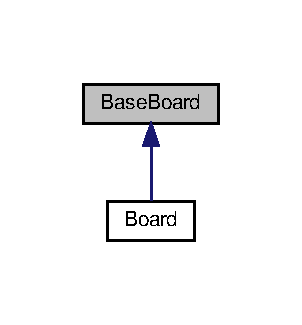
\includegraphics[width=145pt]{class_base_board__inherit__graph}
\end{center}
\end{figure}


Collaboration diagram for Base\+Board\+:\nopagebreak
\begin{figure}[H]
\begin{center}
\leavevmode
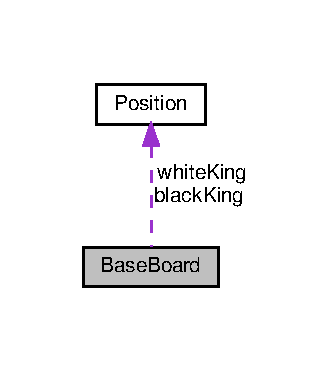
\includegraphics[width=159pt]{class_base_board__coll__graph}
\end{center}
\end{figure}
\subsection*{Public Member Functions}
\begin{DoxyCompactItemize}
\item 
\hyperlink{class_base_board_a120d844f308b6ce12623d5a1ea59ccfb}{Base\+Board} (std\+::vector$<$ std\+::vector$<$ std\+::string $>$$>$ \hyperlink{class_base_board_ae52729f26a30d64d7d643187786e96c2}{board})
\begin{DoxyCompactList}\small\item\em Construct a new Base \hyperlink{class_board}{Board} object. \end{DoxyCompactList}\item 
\hyperlink{_a_i_class_8h_a6e73002e9c84a7986c39d7e80e83dc8d}{board\+\_\+type} \hyperlink{class_base_board_af8f8bdfb2aa7049b30efa40ea9acca20}{get\+Board} ()
\begin{DoxyCompactList}\small\item\em Return board. \end{DoxyCompactList}\item 
void \hyperlink{class_base_board_aeb96bf51fb9bb6fdc42a7abf87de6446}{update\+Board} (int destination\+Column, int destination\+Row, int source\+Column, int source\+Row)
\item 
std\+::vector$<$ std\+::vector$<$ std\+::string $>$ $>$ \hyperlink{class_base_board_ab3a49fb5a7284d66439b785e6add260f}{to\+String} ()
\begin{DoxyCompactList}\small\item\em Used to extract board in vector of strings format to create new board. \end{DoxyCompactList}\item 
void \hyperlink{class_base_board_a1c8fe600a3c0abea281b93cc8be71dd1}{print\+Board\+Cout} ()
\begin{DoxyCompactList}\small\item\em Prints board in console. \end{DoxyCompactList}\item 
\hyperlink{struct_position}{Position} \hyperlink{class_base_board_aebcd17c243c0748897b41fe683dd29f1}{get\+King} (\hyperlink{_piece_8h_ad7595c48bb74c0dd2a7648712a2d4985}{Piece\+Color} king\+Color)
\item 
void \hyperlink{class_base_board_a413af1d87b49a2ee4ce96cb0f165b01a}{set\+King} (\hyperlink{struct_position}{Position} position\+King, \hyperlink{_piece_8h_ad7595c48bb74c0dd2a7648712a2d4985}{Piece\+Color} king\+Color)
\item 
bool \hyperlink{class_base_board_a88d6e53bd8d8dd1f3ec3695fd6c29a81}{is\+Checking} (\hyperlink{_piece_8h_ad7595c48bb74c0dd2a7648712a2d4985}{Piece\+Color} opponent\+Color, std\+::shared\+\_\+ptr$<$ \hyperlink{class_base_board}{Base\+Board} $>$ \hyperlink{class_base_board_ae52729f26a30d64d7d643187786e96c2}{board})
\begin{DoxyCompactList}\small\item\em Is opponent\+Color player checked. \end{DoxyCompactList}\item 
bool \hyperlink{class_base_board_af5c47782cec757ecb8f041925a0d7b7b}{is\+Check\+Mate} (\hyperlink{_piece_8h_ad7595c48bb74c0dd2a7648712a2d4985}{Piece\+Color} opponent\+Color, std\+::shared\+\_\+ptr$<$ \hyperlink{class_base_board}{Base\+Board} $>$ \hyperlink{class_base_board_ae52729f26a30d64d7d643187786e96c2}{board})
\begin{DoxyCompactList}\small\item\em Is opponent\+Color player mated. \end{DoxyCompactList}\end{DoxyCompactItemize}
\subsection*{Private Attributes}
\begin{DoxyCompactItemize}
\item 
\hyperlink{_a_i_class_8h_a6e73002e9c84a7986c39d7e80e83dc8d}{board\+\_\+type} \hyperlink{class_base_board_ae52729f26a30d64d7d643187786e96c2}{board}
\item 
\hyperlink{struct_position}{Position} \hyperlink{class_base_board_a684c71ad408d12f6faf66298c1aeeabc}{white\+King}
\begin{DoxyCompactList}\small\item\em position of white king \end{DoxyCompactList}\item 
\hyperlink{struct_position}{Position} \hyperlink{class_base_board_a9557e923cc07fadd5f0da47ba2a9d230}{black\+King}
\begin{DoxyCompactList}\small\item\em position of black king \end{DoxyCompactList}\end{DoxyCompactItemize}


\subsection{Constructor \& Destructor Documentation}
\mbox{\Hypertarget{class_base_board_a120d844f308b6ce12623d5a1ea59ccfb}\label{class_base_board_a120d844f308b6ce12623d5a1ea59ccfb}} 
\index{Base\+Board@{Base\+Board}!Base\+Board@{Base\+Board}}
\index{Base\+Board@{Base\+Board}!Base\+Board@{Base\+Board}}
\subsubsection{\texorpdfstring{Base\+Board()}{BaseBoard()}}
{\footnotesize\ttfamily Base\+Board\+::\+Base\+Board (\begin{DoxyParamCaption}\item[{std\+::vector$<$ std\+::vector$<$ std\+::string $>$$>$}]{board }\end{DoxyParamCaption})}



Construct a new Base \hyperlink{class_board}{Board} object. 


\begin{DoxyParams}{Parameters}
{\em board} & vector of strings to generate new board \\
\hline
\end{DoxyParams}


\subsection{Member Function Documentation}
\mbox{\Hypertarget{class_base_board_af8f8bdfb2aa7049b30efa40ea9acca20}\label{class_base_board_af8f8bdfb2aa7049b30efa40ea9acca20}} 
\index{Base\+Board@{Base\+Board}!get\+Board@{get\+Board}}
\index{get\+Board@{get\+Board}!Base\+Board@{Base\+Board}}
\subsubsection{\texorpdfstring{get\+Board()}{getBoard()}}
{\footnotesize\ttfamily \hyperlink{_a_i_class_8h_a6e73002e9c84a7986c39d7e80e83dc8d}{board\+\_\+type} Base\+Board\+::get\+Board (\begin{DoxyParamCaption}{ }\end{DoxyParamCaption})}



Return board. 

\mbox{\Hypertarget{class_base_board_aebcd17c243c0748897b41fe683dd29f1}\label{class_base_board_aebcd17c243c0748897b41fe683dd29f1}} 
\index{Base\+Board@{Base\+Board}!get\+King@{get\+King}}
\index{get\+King@{get\+King}!Base\+Board@{Base\+Board}}
\subsubsection{\texorpdfstring{get\+King()}{getKing()}}
{\footnotesize\ttfamily \hyperlink{struct_position}{Position} Base\+Board\+::get\+King (\begin{DoxyParamCaption}\item[{\hyperlink{_piece_8h_ad7595c48bb74c0dd2a7648712a2d4985}{Piece\+Color}}]{king\+Color }\end{DoxyParamCaption})}

\mbox{\Hypertarget{class_base_board_a88d6e53bd8d8dd1f3ec3695fd6c29a81}\label{class_base_board_a88d6e53bd8d8dd1f3ec3695fd6c29a81}} 
\index{Base\+Board@{Base\+Board}!is\+Checking@{is\+Checking}}
\index{is\+Checking@{is\+Checking}!Base\+Board@{Base\+Board}}
\subsubsection{\texorpdfstring{is\+Checking()}{isChecking()}}
{\footnotesize\ttfamily bool Base\+Board\+::is\+Checking (\begin{DoxyParamCaption}\item[{\hyperlink{_piece_8h_ad7595c48bb74c0dd2a7648712a2d4985}{Piece\+Color}}]{opponent\+Color,  }\item[{std\+::shared\+\_\+ptr$<$ \hyperlink{class_base_board}{Base\+Board} $>$}]{board }\end{DoxyParamCaption})}



Is opponent\+Color player checked. 


\begin{DoxyParams}{Parameters}
{\em opponent\+Color} & Color of player, which is checked \\
\hline
{\em board} & Current board \\
\hline
\end{DoxyParams}
\begin{DoxyReturn}{Returns}
true 

false 
\end{DoxyReturn}
\mbox{\Hypertarget{class_base_board_af5c47782cec757ecb8f041925a0d7b7b}\label{class_base_board_af5c47782cec757ecb8f041925a0d7b7b}} 
\index{Base\+Board@{Base\+Board}!is\+Check\+Mate@{is\+Check\+Mate}}
\index{is\+Check\+Mate@{is\+Check\+Mate}!Base\+Board@{Base\+Board}}
\subsubsection{\texorpdfstring{is\+Check\+Mate()}{isCheckMate()}}
{\footnotesize\ttfamily bool Base\+Board\+::is\+Check\+Mate (\begin{DoxyParamCaption}\item[{\hyperlink{_piece_8h_ad7595c48bb74c0dd2a7648712a2d4985}{Piece\+Color}}]{opponent\+Color,  }\item[{std\+::shared\+\_\+ptr$<$ \hyperlink{class_base_board}{Base\+Board} $>$}]{board }\end{DoxyParamCaption})}



Is opponent\+Color player mated. 


\begin{DoxyParams}{Parameters}
{\em opponent\+Color} & Color of player, which is mated \\
\hline
{\em board} & Current board \\
\hline
\end{DoxyParams}
\begin{DoxyReturn}{Returns}
true 

false 
\end{DoxyReturn}
\mbox{\Hypertarget{class_base_board_a1c8fe600a3c0abea281b93cc8be71dd1}\label{class_base_board_a1c8fe600a3c0abea281b93cc8be71dd1}} 
\index{Base\+Board@{Base\+Board}!print\+Board\+Cout@{print\+Board\+Cout}}
\index{print\+Board\+Cout@{print\+Board\+Cout}!Base\+Board@{Base\+Board}}
\subsubsection{\texorpdfstring{print\+Board\+Cout()}{printBoardCout()}}
{\footnotesize\ttfamily void Base\+Board\+::print\+Board\+Cout (\begin{DoxyParamCaption}{ }\end{DoxyParamCaption})}



Prints board in console. 

\mbox{\Hypertarget{class_base_board_a413af1d87b49a2ee4ce96cb0f165b01a}\label{class_base_board_a413af1d87b49a2ee4ce96cb0f165b01a}} 
\index{Base\+Board@{Base\+Board}!set\+King@{set\+King}}
\index{set\+King@{set\+King}!Base\+Board@{Base\+Board}}
\subsubsection{\texorpdfstring{set\+King()}{setKing()}}
{\footnotesize\ttfamily void Base\+Board\+::set\+King (\begin{DoxyParamCaption}\item[{\hyperlink{struct_position}{Position}}]{position\+King,  }\item[{\hyperlink{_piece_8h_ad7595c48bb74c0dd2a7648712a2d4985}{Piece\+Color}}]{king\+Color }\end{DoxyParamCaption})}

\mbox{\Hypertarget{class_base_board_ab3a49fb5a7284d66439b785e6add260f}\label{class_base_board_ab3a49fb5a7284d66439b785e6add260f}} 
\index{Base\+Board@{Base\+Board}!to\+String@{to\+String}}
\index{to\+String@{to\+String}!Base\+Board@{Base\+Board}}
\subsubsection{\texorpdfstring{to\+String()}{toString()}}
{\footnotesize\ttfamily std\+::vector$<$ std\+::vector$<$ std\+::string $>$ $>$ Base\+Board\+::to\+String (\begin{DoxyParamCaption}{ }\end{DoxyParamCaption})}



Used to extract board in vector of strings format to create new board. 

\mbox{\Hypertarget{class_base_board_aeb96bf51fb9bb6fdc42a7abf87de6446}\label{class_base_board_aeb96bf51fb9bb6fdc42a7abf87de6446}} 
\index{Base\+Board@{Base\+Board}!update\+Board@{update\+Board}}
\index{update\+Board@{update\+Board}!Base\+Board@{Base\+Board}}
\subsubsection{\texorpdfstring{update\+Board()}{updateBoard()}}
{\footnotesize\ttfamily void Base\+Board\+::update\+Board (\begin{DoxyParamCaption}\item[{int}]{destination\+Column,  }\item[{int}]{destination\+Row,  }\item[{int}]{source\+Column,  }\item[{int}]{source\+Row }\end{DoxyParamCaption})}


\begin{DoxyParams}{Parameters}
{\em destination\+Column} & \\
\hline
{\em destination\+Row} & \\
\hline
{\em source\+Column} & From where we move \\
\hline
{\em source\+Row} & From where we move \\
\hline
\end{DoxyParams}


\subsection{Member Data Documentation}
\mbox{\Hypertarget{class_base_board_a9557e923cc07fadd5f0da47ba2a9d230}\label{class_base_board_a9557e923cc07fadd5f0da47ba2a9d230}} 
\index{Base\+Board@{Base\+Board}!black\+King@{black\+King}}
\index{black\+King@{black\+King}!Base\+Board@{Base\+Board}}
\subsubsection{\texorpdfstring{black\+King}{blackKing}}
{\footnotesize\ttfamily \hyperlink{struct_position}{Position} Base\+Board\+::black\+King\hspace{0.3cm}{\ttfamily [private]}}



position of black king 

\mbox{\Hypertarget{class_base_board_ae52729f26a30d64d7d643187786e96c2}\label{class_base_board_ae52729f26a30d64d7d643187786e96c2}} 
\index{Base\+Board@{Base\+Board}!board@{board}}
\index{board@{board}!Base\+Board@{Base\+Board}}
\subsubsection{\texorpdfstring{board}{board}}
{\footnotesize\ttfamily \hyperlink{_a_i_class_8h_a6e73002e9c84a7986c39d7e80e83dc8d}{board\+\_\+type} Base\+Board\+::board\hspace{0.3cm}{\ttfamily [private]}}

\mbox{\Hypertarget{class_base_board_a684c71ad408d12f6faf66298c1aeeabc}\label{class_base_board_a684c71ad408d12f6faf66298c1aeeabc}} 
\index{Base\+Board@{Base\+Board}!white\+King@{white\+King}}
\index{white\+King@{white\+King}!Base\+Board@{Base\+Board}}
\subsubsection{\texorpdfstring{white\+King}{whiteKing}}
{\footnotesize\ttfamily \hyperlink{struct_position}{Position} Base\+Board\+::white\+King\hspace{0.3cm}{\ttfamily [private]}}



position of white king 



The documentation for this class was generated from the following files\+:\begin{DoxyCompactItemize}
\item 
lib/\hyperlink{_base_board_8h}{Base\+Board.\+h}\item 
\hyperlink{_base_board_8cc}{Base\+Board.\+cc}\end{DoxyCompactItemize}

\hypertarget{class_bishop}{}\section{Bishop Class Reference}
\label{class_bishop}\index{Bishop@{Bishop}}


{\ttfamily \#include $<$Bishop.\+h$>$}



Inheritance diagram for Bishop\+:\nopagebreak
\begin{figure}[H]
\begin{center}
\leavevmode
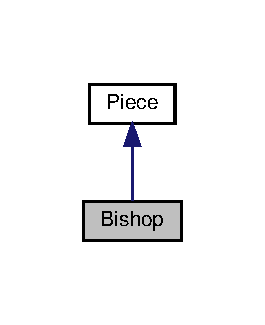
\includegraphics[width=127pt]{class_bishop__inherit__graph}
\end{center}
\end{figure}


Collaboration diagram for Bishop\+:\nopagebreak
\begin{figure}[H]
\begin{center}
\leavevmode
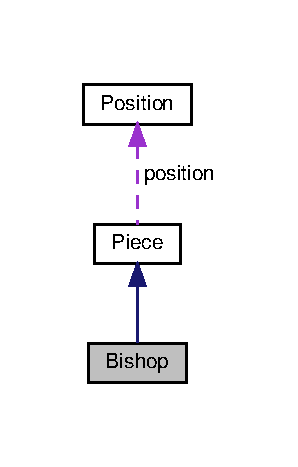
\includegraphics[width=143pt]{class_bishop__coll__graph}
\end{center}
\end{figure}
\subsection*{Public Member Functions}
\begin{DoxyCompactItemize}
\item 
\hyperlink{class_bishop_a89b82abc3b5757e066039e47e398ca66}{Bishop} (int \hyperlink{class_piece_aa8f39e11280395103164f6ae07398c82}{column}, int \hyperlink{class_piece_ac6ef7c474f20562cb629c2452ce0631d}{row}, \hyperlink{_piece_8h_ad7595c48bb74c0dd2a7648712a2d4985}{Piece\+Color} \hyperlink{class_piece_a8dfe0501fe95a1a7618cf5ad3b9fda69}{color}, std\+::string \hyperlink{class_piece_af2fe809fd0d35d167f2419768e49fd3a}{figure\+Name})
\item 
std\+::vector$<$ \hyperlink{struct_position}{Position} $>$ \hyperlink{class_bishop_aed393094415a51e98e0c300da7f79100}{get\+Possible\+Moves} (std\+::shared\+\_\+ptr$<$ \hyperlink{class_base_board}{Base\+Board} $>$, bool) override
\item 
double \hyperlink{class_bishop_a03f53aab9a31cf09c3d252053231eedc}{get\+Position\+Value} () override
\end{DoxyCompactItemize}


\subsection{Constructor \& Destructor Documentation}
\mbox{\Hypertarget{class_bishop_a89b82abc3b5757e066039e47e398ca66}\label{class_bishop_a89b82abc3b5757e066039e47e398ca66}} 
\index{Bishop@{Bishop}!Bishop@{Bishop}}
\index{Bishop@{Bishop}!Bishop@{Bishop}}
\subsubsection{\texorpdfstring{Bishop()}{Bishop()}}
{\footnotesize\ttfamily Bishop\+::\+Bishop (\begin{DoxyParamCaption}\item[{int}]{column,  }\item[{int}]{row,  }\item[{\hyperlink{_piece_8h_ad7595c48bb74c0dd2a7648712a2d4985}{Piece\+Color}}]{color,  }\item[{std\+::string}]{figure\+Name }\end{DoxyParamCaption})\hspace{0.3cm}{\ttfamily [inline]}}



\subsection{Member Function Documentation}
\mbox{\Hypertarget{class_bishop_a03f53aab9a31cf09c3d252053231eedc}\label{class_bishop_a03f53aab9a31cf09c3d252053231eedc}} 
\index{Bishop@{Bishop}!get\+Position\+Value@{get\+Position\+Value}}
\index{get\+Position\+Value@{get\+Position\+Value}!Bishop@{Bishop}}
\subsubsection{\texorpdfstring{get\+Position\+Value()}{getPositionValue()}}
{\footnotesize\ttfamily double Bishop\+::get\+Position\+Value (\begin{DoxyParamCaption}{ }\end{DoxyParamCaption})\hspace{0.3cm}{\ttfamily [override]}, {\ttfamily [virtual]}}



Implements \hyperlink{class_piece_a4adfa58b4f0368c9a5859afcf294e0a4}{Piece}.

\mbox{\Hypertarget{class_bishop_aed393094415a51e98e0c300da7f79100}\label{class_bishop_aed393094415a51e98e0c300da7f79100}} 
\index{Bishop@{Bishop}!get\+Possible\+Moves@{get\+Possible\+Moves}}
\index{get\+Possible\+Moves@{get\+Possible\+Moves}!Bishop@{Bishop}}
\subsubsection{\texorpdfstring{get\+Possible\+Moves()}{getPossibleMoves()}}
{\footnotesize\ttfamily std\+::vector$<$ \hyperlink{struct_position}{Position} $>$ Bishop\+::get\+Possible\+Moves (\begin{DoxyParamCaption}\item[{std\+::shared\+\_\+ptr$<$ \hyperlink{class_base_board}{Base\+Board} $>$}]{board,  }\item[{bool}]{original\+Evaluation }\end{DoxyParamCaption})\hspace{0.3cm}{\ttfamily [override]}, {\ttfamily [virtual]}}



Implements \hyperlink{class_piece_a8891924c280568529878549f59541925}{Piece}.



The documentation for this class was generated from the following files\+:\begin{DoxyCompactItemize}
\item 
lib/\hyperlink{_bishop_8h}{Bishop.\+h}\item 
\hyperlink{_bishop_8cc}{Bishop.\+cc}\end{DoxyCompactItemize}

\hypertarget{class_board}{}\section{Board Class Reference}
\label{class_board}\index{Board@{Board}}


{\ttfamily \#include $<$Board.\+h$>$}



Inheritance diagram for Board\+:\nopagebreak
\begin{figure}[H]
\begin{center}
\leavevmode
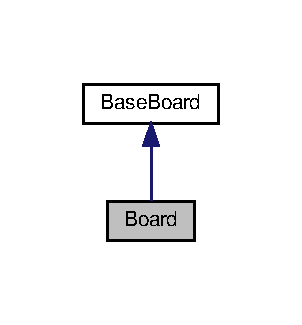
\includegraphics[width=145pt]{class_board__inherit__graph}
\end{center}
\end{figure}


Collaboration diagram for Board\+:\nopagebreak
\begin{figure}[H]
\begin{center}
\leavevmode
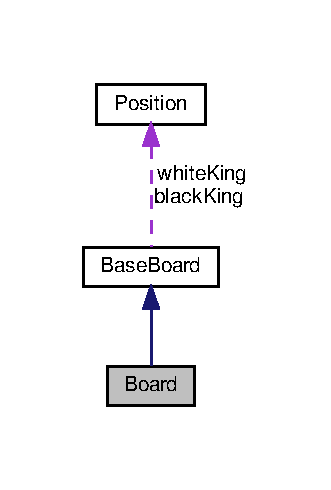
\includegraphics[width=159pt]{class_board__coll__graph}
\end{center}
\end{figure}
\subsection*{Static Public Member Functions}
\begin{DoxyCompactItemize}
\item 
static std\+::shared\+\_\+ptr$<$ \hyperlink{class_board}{Board} $>$ \hyperlink{class_board_ad42eee5655e76255fac9d91eee5d8c64}{get\+Instance} ()
\end{DoxyCompactItemize}
\subsection*{Private Member Functions}
\begin{DoxyCompactItemize}
\item 
\hyperlink{class_board}{Board} \& \hyperlink{class_board_a892306c4b944bfe904b297092763084a}{operator=} (const \hyperlink{class_board}{Board} \&)=delete
\item 
\hyperlink{class_board_a9ee491d4fea680cf69b033374a9fdfcb}{Board} ()
\end{DoxyCompactItemize}
\subsection*{Static Private Attributes}
\begin{DoxyCompactItemize}
\item 
static std\+::shared\+\_\+ptr$<$ \hyperlink{class_board}{Board} $>$ \hyperlink{class_board_a5014ff09a45a8e954b8245357b1544ea}{instance} = nullptr
\end{DoxyCompactItemize}
\subsection*{Additional Inherited Members}


\subsection{Constructor \& Destructor Documentation}
\mbox{\Hypertarget{class_board_a9ee491d4fea680cf69b033374a9fdfcb}\label{class_board_a9ee491d4fea680cf69b033374a9fdfcb}} 
\index{Board@{Board}!Board@{Board}}
\index{Board@{Board}!Board@{Board}}
\subsubsection{\texorpdfstring{Board()}{Board()}}
{\footnotesize\ttfamily Board\+::\+Board (\begin{DoxyParamCaption}{ }\end{DoxyParamCaption})\hspace{0.3cm}{\ttfamily [private]}}



\subsection{Member Function Documentation}
\mbox{\Hypertarget{class_board_ad42eee5655e76255fac9d91eee5d8c64}\label{class_board_ad42eee5655e76255fac9d91eee5d8c64}} 
\index{Board@{Board}!get\+Instance@{get\+Instance}}
\index{get\+Instance@{get\+Instance}!Board@{Board}}
\subsubsection{\texorpdfstring{get\+Instance()}{getInstance()}}
{\footnotesize\ttfamily std\+::shared\+\_\+ptr$<$ \hyperlink{class_board}{Board} $>$ Board\+::get\+Instance (\begin{DoxyParamCaption}{ }\end{DoxyParamCaption})\hspace{0.3cm}{\ttfamily [static]}}

\mbox{\Hypertarget{class_board_a892306c4b944bfe904b297092763084a}\label{class_board_a892306c4b944bfe904b297092763084a}} 
\index{Board@{Board}!operator=@{operator=}}
\index{operator=@{operator=}!Board@{Board}}
\subsubsection{\texorpdfstring{operator=()}{operator=()}}
{\footnotesize\ttfamily \hyperlink{class_board}{Board}\& Board\+::operator= (\begin{DoxyParamCaption}\item[{const \hyperlink{class_board}{Board} \&}]{ }\end{DoxyParamCaption})\hspace{0.3cm}{\ttfamily [private]}, {\ttfamily [delete]}}



\subsection{Member Data Documentation}
\mbox{\Hypertarget{class_board_a5014ff09a45a8e954b8245357b1544ea}\label{class_board_a5014ff09a45a8e954b8245357b1544ea}} 
\index{Board@{Board}!instance@{instance}}
\index{instance@{instance}!Board@{Board}}
\subsubsection{\texorpdfstring{instance}{instance}}
{\footnotesize\ttfamily std\+::shared\+\_\+ptr$<$ \hyperlink{class_board}{Board} $>$ Board\+::instance = nullptr\hspace{0.3cm}{\ttfamily [static]}, {\ttfamily [private]}}



The documentation for this class was generated from the following files\+:\begin{DoxyCompactItemize}
\item 
lib/\hyperlink{_board_8h}{Board.\+h}\item 
\hyperlink{_board_8cc}{Board.\+cc}\end{DoxyCompactItemize}

\hypertarget{class_connector}{}\section{Connector Class Reference}
\label{class_connector}\index{Connector@{Connector}}


{\ttfamily \#include $<$Connector.\+h$>$}

\subsection*{Static Public Member Functions}
\begin{DoxyCompactItemize}
\item 
static bool const \hyperlink{class_connector_a272b6b8e9273bc46499d6b733146579a}{if\+Move\+Possible} (std\+::string dest, std\+::string src)
\item 
static std\+::string const \hyperlink{class_connector_aac754784de647a31ceb1a599cc45550f}{check\+For\+Win} ()
\item 
static std\+::string const \hyperlink{class_connector_ab16b09be62901a7c11f829caac553a17}{opponent\+Move} ()
\end{DoxyCompactItemize}


\subsection{Member Function Documentation}
\mbox{\Hypertarget{class_connector_aac754784de647a31ceb1a599cc45550f}\label{class_connector_aac754784de647a31ceb1a599cc45550f}} 
\index{Connector@{Connector}!check\+For\+Win@{check\+For\+Win}}
\index{check\+For\+Win@{check\+For\+Win}!Connector@{Connector}}
\subsubsection{\texorpdfstring{check\+For\+Win()}{checkForWin()}}
{\footnotesize\ttfamily std\+::string const Connector\+::check\+For\+Win (\begin{DoxyParamCaption}{ }\end{DoxyParamCaption})\hspace{0.3cm}{\ttfamily [static]}}

\mbox{\Hypertarget{class_connector_a272b6b8e9273bc46499d6b733146579a}\label{class_connector_a272b6b8e9273bc46499d6b733146579a}} 
\index{Connector@{Connector}!if\+Move\+Possible@{if\+Move\+Possible}}
\index{if\+Move\+Possible@{if\+Move\+Possible}!Connector@{Connector}}
\subsubsection{\texorpdfstring{if\+Move\+Possible()}{ifMovePossible()}}
{\footnotesize\ttfamily bool const Connector\+::if\+Move\+Possible (\begin{DoxyParamCaption}\item[{std\+::string}]{dest,  }\item[{std\+::string}]{src }\end{DoxyParamCaption})\hspace{0.3cm}{\ttfamily [static]}}

\mbox{\Hypertarget{class_connector_ab16b09be62901a7c11f829caac553a17}\label{class_connector_ab16b09be62901a7c11f829caac553a17}} 
\index{Connector@{Connector}!opponent\+Move@{opponent\+Move}}
\index{opponent\+Move@{opponent\+Move}!Connector@{Connector}}
\subsubsection{\texorpdfstring{opponent\+Move()}{opponentMove()}}
{\footnotesize\ttfamily std\+::string const Connector\+::opponent\+Move (\begin{DoxyParamCaption}{ }\end{DoxyParamCaption})\hspace{0.3cm}{\ttfamily [static]}}



The documentation for this class was generated from the following files\+:\begin{DoxyCompactItemize}
\item 
\hyperlink{_connector_8h}{Connector.\+h}\item 
\hyperlink{_connector_8cc}{Connector.\+cc}\end{DoxyCompactItemize}

\hypertarget{class_king}{}\section{King Class Reference}
\label{class_king}\index{King@{King}}


{\ttfamily \#include $<$King.\+h$>$}



Inheritance diagram for King\+:\nopagebreak
\begin{figure}[H]
\begin{center}
\leavevmode
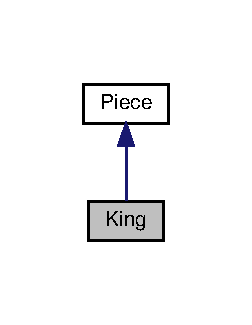
\includegraphics[width=121pt]{class_king__inherit__graph}
\end{center}
\end{figure}


Collaboration diagram for King\+:\nopagebreak
\begin{figure}[H]
\begin{center}
\leavevmode
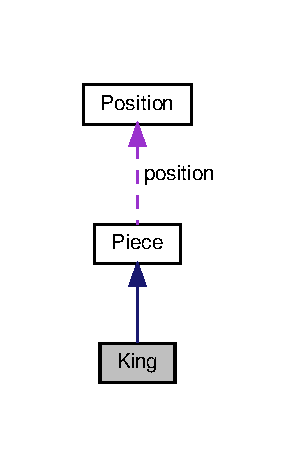
\includegraphics[width=143pt]{class_king__coll__graph}
\end{center}
\end{figure}
\subsection*{Public Member Functions}
\begin{DoxyCompactItemize}
\item 
\hyperlink{class_king_addeee144a4a5076e903652de9ad2f2ce}{King} (int \hyperlink{class_piece_aa8f39e11280395103164f6ae07398c82}{column}, int \hyperlink{class_piece_ac6ef7c474f20562cb629c2452ce0631d}{row}, \hyperlink{_piece_8h_ad7595c48bb74c0dd2a7648712a2d4985}{Piece\+Color} \hyperlink{class_piece_a8dfe0501fe95a1a7618cf5ad3b9fda69}{color})
\item 
std\+::vector$<$ \hyperlink{struct_position}{Position} $>$ \hyperlink{class_king_aa8adeaff952af3bf16ebc1c1c0699d43}{get\+Possible\+Moves} (std\+::shared\+\_\+ptr$<$ \hyperlink{class_base_board}{Base\+Board} $>$ board, bool initialboard) override
\item 
double \hyperlink{class_king_a047413f5f6df784b2fd308f20e356ea4}{get\+Position\+Value} () override
\item 
bool \hyperlink{class_king_a7f58cb2d7d005f03d229af195136b00a}{get\+Castled} ()
\item 
bool \hyperlink{class_king_aecc7387c9b2d6e94b556d416b985b210}{get\+Checked} ()
\item 
void \hyperlink{class_king_a144a81bb4358863415ff41ff851fdbd4}{set\+Castled} (bool \hyperlink{class_king_af1d6712d05b377b1989d7625e5aceb38}{castled})
\item 
void \hyperlink{class_king_af55ffa8c550debf65d6b64a91472626b}{set\+Checked} (bool \hyperlink{class_king_afd51388c6257f775868f8bde25591a31}{checked})
\end{DoxyCompactItemize}
\subsection*{Private Attributes}
\begin{DoxyCompactItemize}
\item 
bool \hyperlink{class_king_af1d6712d05b377b1989d7625e5aceb38}{castled} = false
\item 
bool \hyperlink{class_king_afd51388c6257f775868f8bde25591a31}{checked} = false
\end{DoxyCompactItemize}


\subsection{Constructor \& Destructor Documentation}
\mbox{\Hypertarget{class_king_addeee144a4a5076e903652de9ad2f2ce}\label{class_king_addeee144a4a5076e903652de9ad2f2ce}} 
\index{King@{King}!King@{King}}
\index{King@{King}!King@{King}}
\subsubsection{\texorpdfstring{King()}{King()}}
{\footnotesize\ttfamily King\+::\+King (\begin{DoxyParamCaption}\item[{int}]{column,  }\item[{int}]{row,  }\item[{\hyperlink{_piece_8h_ad7595c48bb74c0dd2a7648712a2d4985}{Piece\+Color}}]{color }\end{DoxyParamCaption})\hspace{0.3cm}{\ttfamily [inline]}}



\subsection{Member Function Documentation}
\mbox{\Hypertarget{class_king_a7f58cb2d7d005f03d229af195136b00a}\label{class_king_a7f58cb2d7d005f03d229af195136b00a}} 
\index{King@{King}!get\+Castled@{get\+Castled}}
\index{get\+Castled@{get\+Castled}!King@{King}}
\subsubsection{\texorpdfstring{get\+Castled()}{getCastled()}}
{\footnotesize\ttfamily bool King\+::get\+Castled (\begin{DoxyParamCaption}{ }\end{DoxyParamCaption})}

\mbox{\Hypertarget{class_king_aecc7387c9b2d6e94b556d416b985b210}\label{class_king_aecc7387c9b2d6e94b556d416b985b210}} 
\index{King@{King}!get\+Checked@{get\+Checked}}
\index{get\+Checked@{get\+Checked}!King@{King}}
\subsubsection{\texorpdfstring{get\+Checked()}{getChecked()}}
{\footnotesize\ttfamily bool King\+::get\+Checked (\begin{DoxyParamCaption}{ }\end{DoxyParamCaption})}

\mbox{\Hypertarget{class_king_a047413f5f6df784b2fd308f20e356ea4}\label{class_king_a047413f5f6df784b2fd308f20e356ea4}} 
\index{King@{King}!get\+Position\+Value@{get\+Position\+Value}}
\index{get\+Position\+Value@{get\+Position\+Value}!King@{King}}
\subsubsection{\texorpdfstring{get\+Position\+Value()}{getPositionValue()}}
{\footnotesize\ttfamily double King\+::get\+Position\+Value (\begin{DoxyParamCaption}{ }\end{DoxyParamCaption})\hspace{0.3cm}{\ttfamily [override]}, {\ttfamily [virtual]}}



Implements \hyperlink{class_piece_a4adfa58b4f0368c9a5859afcf294e0a4}{Piece}.

\mbox{\Hypertarget{class_king_aa8adeaff952af3bf16ebc1c1c0699d43}\label{class_king_aa8adeaff952af3bf16ebc1c1c0699d43}} 
\index{King@{King}!get\+Possible\+Moves@{get\+Possible\+Moves}}
\index{get\+Possible\+Moves@{get\+Possible\+Moves}!King@{King}}
\subsubsection{\texorpdfstring{get\+Possible\+Moves()}{getPossibleMoves()}}
{\footnotesize\ttfamily std\+::vector$<$ \hyperlink{struct_position}{Position} $>$ King\+::get\+Possible\+Moves (\begin{DoxyParamCaption}\item[{std\+::shared\+\_\+ptr$<$ \hyperlink{class_base_board}{Base\+Board} $>$}]{board,  }\item[{bool}]{initialboard }\end{DoxyParamCaption})\hspace{0.3cm}{\ttfamily [override]}, {\ttfamily [virtual]}}



Implements \hyperlink{class_piece_a8891924c280568529878549f59541925}{Piece}.

\mbox{\Hypertarget{class_king_a144a81bb4358863415ff41ff851fdbd4}\label{class_king_a144a81bb4358863415ff41ff851fdbd4}} 
\index{King@{King}!set\+Castled@{set\+Castled}}
\index{set\+Castled@{set\+Castled}!King@{King}}
\subsubsection{\texorpdfstring{set\+Castled()}{setCastled()}}
{\footnotesize\ttfamily void King\+::set\+Castled (\begin{DoxyParamCaption}\item[{bool}]{castled }\end{DoxyParamCaption})}

\mbox{\Hypertarget{class_king_af55ffa8c550debf65d6b64a91472626b}\label{class_king_af55ffa8c550debf65d6b64a91472626b}} 
\index{King@{King}!set\+Checked@{set\+Checked}}
\index{set\+Checked@{set\+Checked}!King@{King}}
\subsubsection{\texorpdfstring{set\+Checked()}{setChecked()}}
{\footnotesize\ttfamily void King\+::set\+Checked (\begin{DoxyParamCaption}\item[{bool}]{checked }\end{DoxyParamCaption})}



\subsection{Member Data Documentation}
\mbox{\Hypertarget{class_king_af1d6712d05b377b1989d7625e5aceb38}\label{class_king_af1d6712d05b377b1989d7625e5aceb38}} 
\index{King@{King}!castled@{castled}}
\index{castled@{castled}!King@{King}}
\subsubsection{\texorpdfstring{castled}{castled}}
{\footnotesize\ttfamily bool King\+::castled = false\hspace{0.3cm}{\ttfamily [private]}}

\mbox{\Hypertarget{class_king_afd51388c6257f775868f8bde25591a31}\label{class_king_afd51388c6257f775868f8bde25591a31}} 
\index{King@{King}!checked@{checked}}
\index{checked@{checked}!King@{King}}
\subsubsection{\texorpdfstring{checked}{checked}}
{\footnotesize\ttfamily bool King\+::checked = false\hspace{0.3cm}{\ttfamily [private]}}



The documentation for this class was generated from the following files\+:\begin{DoxyCompactItemize}
\item 
lib/\hyperlink{_king_8h}{King.\+h}\item 
\hyperlink{_king_8cc}{King.\+cc}\end{DoxyCompactItemize}

\hypertarget{class_knight}{}\section{Knight Class Reference}
\label{class_knight}\index{Knight@{Knight}}


{\ttfamily \#include $<$Knight.\+h$>$}



Inheritance diagram for Knight\+:\nopagebreak
\begin{figure}[H]
\begin{center}
\leavevmode
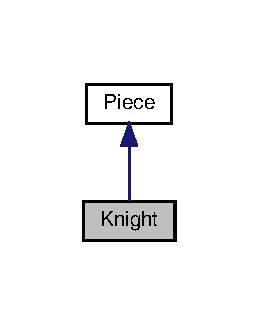
\includegraphics[width=124pt]{class_knight__inherit__graph}
\end{center}
\end{figure}


Collaboration diagram for Knight\+:\nopagebreak
\begin{figure}[H]
\begin{center}
\leavevmode
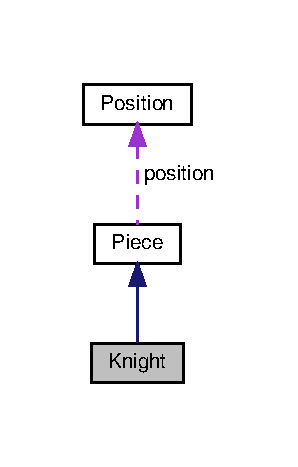
\includegraphics[width=143pt]{class_knight__coll__graph}
\end{center}
\end{figure}
\subsection*{Public Member Functions}
\begin{DoxyCompactItemize}
\item 
\hyperlink{class_knight_ad56d98cc438c67c44d5d18c3a51db1f0}{Knight} (int \hyperlink{class_piece_aa8f39e11280395103164f6ae07398c82}{column}, int \hyperlink{class_piece_ac6ef7c474f20562cb629c2452ce0631d}{row}, \hyperlink{_piece_8h_ad7595c48bb74c0dd2a7648712a2d4985}{Piece\+Color} \hyperlink{class_piece_a8dfe0501fe95a1a7618cf5ad3b9fda69}{color}, std\+::string \hyperlink{class_piece_af2fe809fd0d35d167f2419768e49fd3a}{figure\+Name})
\item 
std\+::vector$<$ \hyperlink{struct_position}{Position} $>$ \hyperlink{class_knight_a65f4e2cdeafefd7e4a7d3c9bca051a5a}{get\+Possible\+Moves} (std\+::shared\+\_\+ptr$<$ \hyperlink{class_base_board}{Base\+Board} $>$, bool) override
\item 
double \hyperlink{class_knight_aa5116e2b3cbbb576283015565b6261a1}{get\+Position\+Value} () override
\end{DoxyCompactItemize}


\subsection{Constructor \& Destructor Documentation}
\mbox{\Hypertarget{class_knight_ad56d98cc438c67c44d5d18c3a51db1f0}\label{class_knight_ad56d98cc438c67c44d5d18c3a51db1f0}} 
\index{Knight@{Knight}!Knight@{Knight}}
\index{Knight@{Knight}!Knight@{Knight}}
\subsubsection{\texorpdfstring{Knight()}{Knight()}}
{\footnotesize\ttfamily Knight\+::\+Knight (\begin{DoxyParamCaption}\item[{int}]{column,  }\item[{int}]{row,  }\item[{\hyperlink{_piece_8h_ad7595c48bb74c0dd2a7648712a2d4985}{Piece\+Color}}]{color,  }\item[{std\+::string}]{figure\+Name }\end{DoxyParamCaption})\hspace{0.3cm}{\ttfamily [inline]}}



\subsection{Member Function Documentation}
\mbox{\Hypertarget{class_knight_aa5116e2b3cbbb576283015565b6261a1}\label{class_knight_aa5116e2b3cbbb576283015565b6261a1}} 
\index{Knight@{Knight}!get\+Position\+Value@{get\+Position\+Value}}
\index{get\+Position\+Value@{get\+Position\+Value}!Knight@{Knight}}
\subsubsection{\texorpdfstring{get\+Position\+Value()}{getPositionValue()}}
{\footnotesize\ttfamily double Knight\+::get\+Position\+Value (\begin{DoxyParamCaption}{ }\end{DoxyParamCaption})\hspace{0.3cm}{\ttfamily [override]}, {\ttfamily [virtual]}}



Implements \hyperlink{class_piece_a4adfa58b4f0368c9a5859afcf294e0a4}{Piece}.

\mbox{\Hypertarget{class_knight_a65f4e2cdeafefd7e4a7d3c9bca051a5a}\label{class_knight_a65f4e2cdeafefd7e4a7d3c9bca051a5a}} 
\index{Knight@{Knight}!get\+Possible\+Moves@{get\+Possible\+Moves}}
\index{get\+Possible\+Moves@{get\+Possible\+Moves}!Knight@{Knight}}
\subsubsection{\texorpdfstring{get\+Possible\+Moves()}{getPossibleMoves()}}
{\footnotesize\ttfamily std\+::vector$<$ \hyperlink{struct_position}{Position} $>$ Knight\+::get\+Possible\+Moves (\begin{DoxyParamCaption}\item[{std\+::shared\+\_\+ptr$<$ \hyperlink{class_base_board}{Base\+Board} $>$}]{board,  }\item[{bool}]{original\+Evaluation }\end{DoxyParamCaption})\hspace{0.3cm}{\ttfamily [override]}, {\ttfamily [virtual]}}



Implements \hyperlink{class_piece_a8891924c280568529878549f59541925}{Piece}.



The documentation for this class was generated from the following files\+:\begin{DoxyCompactItemize}
\item 
lib/\hyperlink{_knight_8h}{Knight.\+h}\item 
\hyperlink{_knight_8cc}{Knight.\+cc}\end{DoxyCompactItemize}

\hypertarget{struct_move_packet}{}\section{Move\+Packet Struct Reference}
\label{struct_move_packet}\index{Move\+Packet@{Move\+Packet}}


{\ttfamily \#include $<$A\+I\+Class.\+h$>$}

\subsection*{Public Attributes}
\begin{DoxyCompactItemize}
\item 
int \hyperlink{struct_move_packet_ac47381c0c93b204e2e9a8251537f0118}{src\+\_\+row}
\item 
int \hyperlink{struct_move_packet_a174bf6f0d24a094e8cd3a8af0547dc9f}{src\+\_\+col}
\item 
int \hyperlink{struct_move_packet_aa4e9c53e9b13bd1e01bcbe36aece9321}{dest\+\_\+row}
\item 
int \hyperlink{struct_move_packet_a76e460ec3c99d9c07e365419bfec9c79}{dest\+\_\+col}
\item 
double \hyperlink{struct_move_packet_ae502e180cfc98f90b24b9d5521f80161}{score}
\end{DoxyCompactItemize}


\subsection{Member Data Documentation}
\mbox{\Hypertarget{struct_move_packet_a76e460ec3c99d9c07e365419bfec9c79}\label{struct_move_packet_a76e460ec3c99d9c07e365419bfec9c79}} 
\index{Move\+Packet@{Move\+Packet}!dest\+\_\+col@{dest\+\_\+col}}
\index{dest\+\_\+col@{dest\+\_\+col}!Move\+Packet@{Move\+Packet}}
\subsubsection{\texorpdfstring{dest\+\_\+col}{dest\_col}}
{\footnotesize\ttfamily int Move\+Packet\+::dest\+\_\+col}

\mbox{\Hypertarget{struct_move_packet_aa4e9c53e9b13bd1e01bcbe36aece9321}\label{struct_move_packet_aa4e9c53e9b13bd1e01bcbe36aece9321}} 
\index{Move\+Packet@{Move\+Packet}!dest\+\_\+row@{dest\+\_\+row}}
\index{dest\+\_\+row@{dest\+\_\+row}!Move\+Packet@{Move\+Packet}}
\subsubsection{\texorpdfstring{dest\+\_\+row}{dest\_row}}
{\footnotesize\ttfamily int Move\+Packet\+::dest\+\_\+row}

\mbox{\Hypertarget{struct_move_packet_ae502e180cfc98f90b24b9d5521f80161}\label{struct_move_packet_ae502e180cfc98f90b24b9d5521f80161}} 
\index{Move\+Packet@{Move\+Packet}!score@{score}}
\index{score@{score}!Move\+Packet@{Move\+Packet}}
\subsubsection{\texorpdfstring{score}{score}}
{\footnotesize\ttfamily double Move\+Packet\+::score}

\mbox{\Hypertarget{struct_move_packet_a174bf6f0d24a094e8cd3a8af0547dc9f}\label{struct_move_packet_a174bf6f0d24a094e8cd3a8af0547dc9f}} 
\index{Move\+Packet@{Move\+Packet}!src\+\_\+col@{src\+\_\+col}}
\index{src\+\_\+col@{src\+\_\+col}!Move\+Packet@{Move\+Packet}}
\subsubsection{\texorpdfstring{src\+\_\+col}{src\_col}}
{\footnotesize\ttfamily int Move\+Packet\+::src\+\_\+col}

\mbox{\Hypertarget{struct_move_packet_ac47381c0c93b204e2e9a8251537f0118}\label{struct_move_packet_ac47381c0c93b204e2e9a8251537f0118}} 
\index{Move\+Packet@{Move\+Packet}!src\+\_\+row@{src\+\_\+row}}
\index{src\+\_\+row@{src\+\_\+row}!Move\+Packet@{Move\+Packet}}
\subsubsection{\texorpdfstring{src\+\_\+row}{src\_row}}
{\footnotesize\ttfamily int Move\+Packet\+::src\+\_\+row}



The documentation for this struct was generated from the following file\+:\begin{DoxyCompactItemize}
\item 
A\+I/\hyperlink{_a_i_class_8h}{A\+I\+Class.\+h}\end{DoxyCompactItemize}

\hypertarget{class_pawn}{}\section{Pawn Class Reference}
\label{class_pawn}\index{Pawn@{Pawn}}


{\ttfamily \#include $<$Pawn.\+h$>$}



Inheritance diagram for Pawn\+:\nopagebreak
\begin{figure}[H]
\begin{center}
\leavevmode
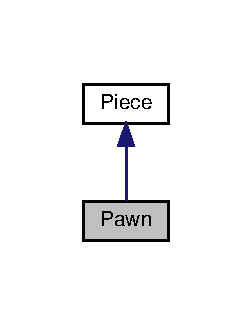
\includegraphics[width=121pt]{class_pawn__inherit__graph}
\end{center}
\end{figure}


Collaboration diagram for Pawn\+:\nopagebreak
\begin{figure}[H]
\begin{center}
\leavevmode
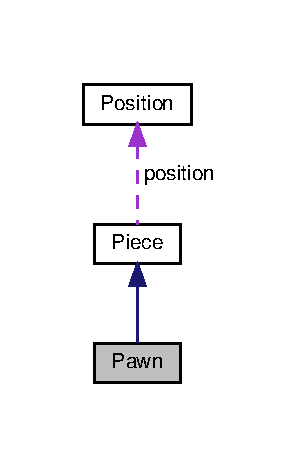
\includegraphics[width=143pt]{class_pawn__coll__graph}
\end{center}
\end{figure}
\subsection*{Public Member Functions}
\begin{DoxyCompactItemize}
\item 
\hyperlink{class_pawn_a560979144129b551c2a27b2eb637d652}{Pawn} (int \hyperlink{class_piece_aa8f39e11280395103164f6ae07398c82}{column}, int \hyperlink{class_piece_ac6ef7c474f20562cb629c2452ce0631d}{row}, \hyperlink{_piece_8h_ad7595c48bb74c0dd2a7648712a2d4985}{Piece\+Color} \hyperlink{class_piece_a8dfe0501fe95a1a7618cf5ad3b9fda69}{color})
\item 
std\+::vector$<$ \hyperlink{struct_position}{Position} $>$ \hyperlink{class_pawn_af83688d6061d4dc14274af99bcbd2614}{get\+Possible\+Moves} (std\+::shared\+\_\+ptr$<$ \hyperlink{class_base_board}{Base\+Board} $>$, bool) override
\item 
double \hyperlink{class_pawn_a332e70ab65f480521428aa87c7cd2ef9}{get\+Position\+Value} () override
\end{DoxyCompactItemize}
\subsection*{Private Attributes}
\begin{DoxyCompactItemize}
\item 
bool \hyperlink{class_pawn_aac8df37fd58c41fe91460325e5447464}{moved} = false
\end{DoxyCompactItemize}


\subsection{Constructor \& Destructor Documentation}
\mbox{\Hypertarget{class_pawn_a560979144129b551c2a27b2eb637d652}\label{class_pawn_a560979144129b551c2a27b2eb637d652}} 
\index{Pawn@{Pawn}!Pawn@{Pawn}}
\index{Pawn@{Pawn}!Pawn@{Pawn}}
\subsubsection{\texorpdfstring{Pawn()}{Pawn()}}
{\footnotesize\ttfamily Pawn\+::\+Pawn (\begin{DoxyParamCaption}\item[{int}]{column,  }\item[{int}]{row,  }\item[{\hyperlink{_piece_8h_ad7595c48bb74c0dd2a7648712a2d4985}{Piece\+Color}}]{color }\end{DoxyParamCaption})\hspace{0.3cm}{\ttfamily [inline]}}



\subsection{Member Function Documentation}
\mbox{\Hypertarget{class_pawn_a332e70ab65f480521428aa87c7cd2ef9}\label{class_pawn_a332e70ab65f480521428aa87c7cd2ef9}} 
\index{Pawn@{Pawn}!get\+Position\+Value@{get\+Position\+Value}}
\index{get\+Position\+Value@{get\+Position\+Value}!Pawn@{Pawn}}
\subsubsection{\texorpdfstring{get\+Position\+Value()}{getPositionValue()}}
{\footnotesize\ttfamily double Pawn\+::get\+Position\+Value (\begin{DoxyParamCaption}{ }\end{DoxyParamCaption})\hspace{0.3cm}{\ttfamily [override]}, {\ttfamily [virtual]}}



Implements \hyperlink{class_piece_a4adfa58b4f0368c9a5859afcf294e0a4}{Piece}.

\mbox{\Hypertarget{class_pawn_af83688d6061d4dc14274af99bcbd2614}\label{class_pawn_af83688d6061d4dc14274af99bcbd2614}} 
\index{Pawn@{Pawn}!get\+Possible\+Moves@{get\+Possible\+Moves}}
\index{get\+Possible\+Moves@{get\+Possible\+Moves}!Pawn@{Pawn}}
\subsubsection{\texorpdfstring{get\+Possible\+Moves()}{getPossibleMoves()}}
{\footnotesize\ttfamily std\+::vector$<$ \hyperlink{struct_position}{Position} $>$ Pawn\+::get\+Possible\+Moves (\begin{DoxyParamCaption}\item[{std\+::shared\+\_\+ptr$<$ \hyperlink{class_base_board}{Base\+Board} $>$}]{board,  }\item[{bool}]{original\+Evaluation }\end{DoxyParamCaption})\hspace{0.3cm}{\ttfamily [override]}, {\ttfamily [virtual]}}



Implements \hyperlink{class_piece_a8891924c280568529878549f59541925}{Piece}.



\subsection{Member Data Documentation}
\mbox{\Hypertarget{class_pawn_aac8df37fd58c41fe91460325e5447464}\label{class_pawn_aac8df37fd58c41fe91460325e5447464}} 
\index{Pawn@{Pawn}!moved@{moved}}
\index{moved@{moved}!Pawn@{Pawn}}
\subsubsection{\texorpdfstring{moved}{moved}}
{\footnotesize\ttfamily bool Pawn\+::moved = false\hspace{0.3cm}{\ttfamily [private]}}



The documentation for this class was generated from the following files\+:\begin{DoxyCompactItemize}
\item 
lib/\hyperlink{_pawn_8h}{Pawn.\+h}\item 
\hyperlink{_pawn_8cc}{Pawn.\+cc}\end{DoxyCompactItemize}

\hypertarget{class_piece}{}\section{Piece Class Reference}
\label{class_piece}\index{Piece@{Piece}}


{\ttfamily \#include $<$Piece.\+h$>$}



Inheritance diagram for Piece\+:\nopagebreak
\begin{figure}[H]
\begin{center}
\leavevmode
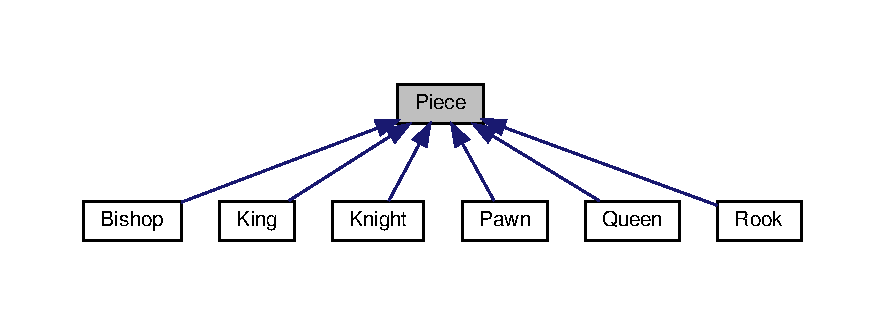
\includegraphics[width=350pt]{class_piece__inherit__graph}
\end{center}
\end{figure}


Collaboration diagram for Piece\+:\nopagebreak
\begin{figure}[H]
\begin{center}
\leavevmode
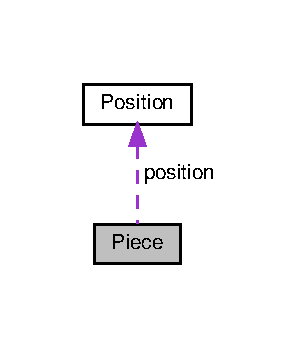
\includegraphics[width=143pt]{class_piece__coll__graph}
\end{center}
\end{figure}
\subsection*{Public Member Functions}
\begin{DoxyCompactItemize}
\item 
\hyperlink{class_piece_a1ae0a039406ce1ca4eebc4465426bf25}{Piece} (int, int, \hyperlink{_piece_8h_ad7595c48bb74c0dd2a7648712a2d4985}{Piece\+Color})
\item 
\hyperlink{class_piece_a98d2204a49a52df4cda971aa669e6796}{Piece} (\hyperlink{struct_position}{Position}, \hyperlink{_piece_8h_ad7595c48bb74c0dd2a7648712a2d4985}{Piece\+Color})
\item 
void \hyperlink{class_piece_a5b8c0f65eb850c91ae148501cd15adbf}{set\+Color} (\hyperlink{_piece_8h_ad7595c48bb74c0dd2a7648712a2d4985}{Piece\+Color})
\item 
void \hyperlink{class_piece_a604cbeae62b4358425d046bc5d737a39}{set\+Row} (int)
\item 
void \hyperlink{class_piece_a826ba56a44a5bf2e1ecdea849f2581d3}{set\+Column} (int)
\item 
void \hyperlink{class_piece_a459865f830ff8c199cfca49f5d89b806}{set\+Position} (\hyperlink{struct_position}{Position})
\item 
void \hyperlink{class_piece_a0ff1ca92370da533f6ef421dc09741f8}{set\+Moved} ()
\item 
void \hyperlink{class_piece_aad0fbfd687db57c60b5b4585b67f387d}{set\+Occupied} (bool)
\item 
void \hyperlink{class_piece_ad63e838ac5edfe8abab7211fc79e5a82}{set\+Moves} (std\+::vector$<$ \hyperlink{struct_position}{Position} $>$)
\item 
void \hyperlink{class_piece_a16971e1511ab403ede566b4fdbbab8a8}{set\+Figure\+Name} (std\+::string)
\item 
bool \hyperlink{class_piece_aa45b0c7c5552437dfd9d4567d2c7e7dd}{is\+Checking} (\hyperlink{struct_position}{Position} position\+Piece, \hyperlink{struct_position}{Position} position\+King)
\item 
\hyperlink{struct_position}{Position} \hyperlink{class_piece_a8537f9ebe9b135e3e5da99f385a90042}{get\+King} (std\+::shared\+\_\+ptr$<$ \hyperlink{class_base_board}{Base\+Board} $>$, \hyperlink{_piece_8h_ad7595c48bb74c0dd2a7648712a2d4985}{Piece\+Color} piece\+Color)
\item 
std\+::vector$<$ \hyperlink{struct_position}{Position} $>$ \hyperlink{class_piece_a9cb5fe774dcb187ce20ff18c93269e3f}{evaluate\+Check} (std\+::shared\+\_\+ptr$<$ \hyperlink{class_base_board}{Base\+Board} $>$ board, bool initialboard)
\item 
virtual std\+::vector$<$ \hyperlink{struct_position}{Position} $>$ \hyperlink{class_piece_a8891924c280568529878549f59541925}{get\+Possible\+Moves} (std\+::shared\+\_\+ptr$<$ \hyperlink{class_base_board}{Base\+Board} $>$, bool=true)=0
\item 
virtual double \hyperlink{class_piece_a4adfa58b4f0368c9a5859afcf294e0a4}{get\+Position\+Value} ()=0
\item 
\hyperlink{_piece_8h_ad7595c48bb74c0dd2a7648712a2d4985}{Piece\+Color} \hyperlink{class_piece_a184ce3e31f7b4d8a3d616a60fe60522e}{get\+Color} ()
\item 
int \hyperlink{class_piece_a3396fcbbe54260076bf2f6a39b0fb920}{get\+Column} ()
\item 
int \hyperlink{class_piece_a070f593242fb8417429ac989184e682b}{get\+Row} ()
\item 
\hyperlink{struct_position}{Position} \hyperlink{class_piece_a2dee0ebeffdb733e17574471c441e06d}{get\+Position} ()
\item 
bool \hyperlink{class_piece_ad23431fecbbedcff824dd38ffa6a47a1}{get\+Moved} ()
\item 
bool \hyperlink{class_piece_abde93826a7b04b9e0f9739b11df0629e}{get\+Occupied} ()
\item 
std\+::vector$<$ \hyperlink{struct_position}{Position} $>$ \hyperlink{class_piece_a10eddaa8ade831cfee1c17b94bfcac09}{get\+Moves} ()
\item 
std\+::string \hyperlink{class_piece_a094d0d28514219ab3f155d9241bb8f22}{get\+Figure\+Name} ()
\end{DoxyCompactItemize}
\subsection*{Private Attributes}
\begin{DoxyCompactItemize}
\item 
std\+::string \hyperlink{class_piece_af2fe809fd0d35d167f2419768e49fd3a}{figure\+Name}
\item 
\hyperlink{_piece_8h_ad7595c48bb74c0dd2a7648712a2d4985}{Piece\+Color} \hyperlink{class_piece_a8dfe0501fe95a1a7618cf5ad3b9fda69}{color} = \hyperlink{_piece_8h_ad7595c48bb74c0dd2a7648712a2d4985af77fb67151d0c18d397069ad8c271ba3}{B\+L\+A\+CK}
\item 
\hyperlink{struct_position}{Position} \hyperlink{class_piece_a818688fca11efe2957b0605bb2976f49}{position}
\item 
int \hyperlink{class_piece_aa8f39e11280395103164f6ae07398c82}{column}
\item 
int \hyperlink{class_piece_ac6ef7c474f20562cb629c2452ce0631d}{row}
\item 
bool \hyperlink{class_piece_a063178abee009388c7d07e112efc3be4}{occupied} = true
\item 
bool \hyperlink{class_piece_ad1320904ecb8565e96d6020f857c990c}{moved} = false
\item 
std\+::vector$<$ \hyperlink{struct_position}{Position} $>$ \hyperlink{class_piece_a22ef4ba5ffcc5767149332320230373e}{moves}
\end{DoxyCompactItemize}
\subsection*{Friends}
\begin{DoxyCompactItemize}
\item 
std\+::ostream \& \hyperlink{class_piece_a2030184caa17f039eb2a026a6dbc7d23}{operator$<$$<$} (std\+::ostream \&out, const \hyperlink{class_piece}{Piece} \&c)
\end{DoxyCompactItemize}


\subsection{Constructor \& Destructor Documentation}
\mbox{\Hypertarget{class_piece_a1ae0a039406ce1ca4eebc4465426bf25}\label{class_piece_a1ae0a039406ce1ca4eebc4465426bf25}} 
\index{Piece@{Piece}!Piece@{Piece}}
\index{Piece@{Piece}!Piece@{Piece}}
\subsubsection{\texorpdfstring{Piece()}{Piece()}\hspace{0.1cm}{\footnotesize\ttfamily [1/2]}}
{\footnotesize\ttfamily Piece\+::\+Piece (\begin{DoxyParamCaption}\item[{int}]{column,  }\item[{int}]{row,  }\item[{\hyperlink{_piece_8h_ad7595c48bb74c0dd2a7648712a2d4985}{Piece\+Color}}]{color }\end{DoxyParamCaption})}

\mbox{\Hypertarget{class_piece_a98d2204a49a52df4cda971aa669e6796}\label{class_piece_a98d2204a49a52df4cda971aa669e6796}} 
\index{Piece@{Piece}!Piece@{Piece}}
\index{Piece@{Piece}!Piece@{Piece}}
\subsubsection{\texorpdfstring{Piece()}{Piece()}\hspace{0.1cm}{\footnotesize\ttfamily [2/2]}}
{\footnotesize\ttfamily Piece\+::\+Piece (\begin{DoxyParamCaption}\item[{\hyperlink{struct_position}{Position}}]{,  }\item[{\hyperlink{_piece_8h_ad7595c48bb74c0dd2a7648712a2d4985}{Piece\+Color}}]{ }\end{DoxyParamCaption})\hspace{0.3cm}{\ttfamily [inline]}}



\subsection{Member Function Documentation}
\mbox{\Hypertarget{class_piece_a9cb5fe774dcb187ce20ff18c93269e3f}\label{class_piece_a9cb5fe774dcb187ce20ff18c93269e3f}} 
\index{Piece@{Piece}!evaluate\+Check@{evaluate\+Check}}
\index{evaluate\+Check@{evaluate\+Check}!Piece@{Piece}}
\subsubsection{\texorpdfstring{evaluate\+Check()}{evaluateCheck()}}
{\footnotesize\ttfamily std\+::vector$<$ \hyperlink{struct_position}{Position} $>$ Piece\+::evaluate\+Check (\begin{DoxyParamCaption}\item[{std\+::shared\+\_\+ptr$<$ \hyperlink{class_base_board}{Base\+Board} $>$}]{board,  }\item[{bool}]{initialboard }\end{DoxyParamCaption})}

\mbox{\Hypertarget{class_piece_a184ce3e31f7b4d8a3d616a60fe60522e}\label{class_piece_a184ce3e31f7b4d8a3d616a60fe60522e}} 
\index{Piece@{Piece}!get\+Color@{get\+Color}}
\index{get\+Color@{get\+Color}!Piece@{Piece}}
\subsubsection{\texorpdfstring{get\+Color()}{getColor()}}
{\footnotesize\ttfamily \hyperlink{_piece_8h_ad7595c48bb74c0dd2a7648712a2d4985}{Piece\+Color} Piece\+::get\+Color (\begin{DoxyParamCaption}{ }\end{DoxyParamCaption})}

\mbox{\Hypertarget{class_piece_a3396fcbbe54260076bf2f6a39b0fb920}\label{class_piece_a3396fcbbe54260076bf2f6a39b0fb920}} 
\index{Piece@{Piece}!get\+Column@{get\+Column}}
\index{get\+Column@{get\+Column}!Piece@{Piece}}
\subsubsection{\texorpdfstring{get\+Column()}{getColumn()}}
{\footnotesize\ttfamily int Piece\+::get\+Column (\begin{DoxyParamCaption}{ }\end{DoxyParamCaption})}

\mbox{\Hypertarget{class_piece_a094d0d28514219ab3f155d9241bb8f22}\label{class_piece_a094d0d28514219ab3f155d9241bb8f22}} 
\index{Piece@{Piece}!get\+Figure\+Name@{get\+Figure\+Name}}
\index{get\+Figure\+Name@{get\+Figure\+Name}!Piece@{Piece}}
\subsubsection{\texorpdfstring{get\+Figure\+Name()}{getFigureName()}}
{\footnotesize\ttfamily std\+::string Piece\+::get\+Figure\+Name (\begin{DoxyParamCaption}{ }\end{DoxyParamCaption})}

\mbox{\Hypertarget{class_piece_a8537f9ebe9b135e3e5da99f385a90042}\label{class_piece_a8537f9ebe9b135e3e5da99f385a90042}} 
\index{Piece@{Piece}!get\+King@{get\+King}}
\index{get\+King@{get\+King}!Piece@{Piece}}
\subsubsection{\texorpdfstring{get\+King()}{getKing()}}
{\footnotesize\ttfamily \hyperlink{struct_position}{Position} Piece\+::get\+King (\begin{DoxyParamCaption}\item[{std\+::shared\+\_\+ptr$<$ \hyperlink{class_base_board}{Base\+Board} $>$}]{board,  }\item[{\hyperlink{_piece_8h_ad7595c48bb74c0dd2a7648712a2d4985}{Piece\+Color}}]{piece\+Color }\end{DoxyParamCaption})}

\mbox{\Hypertarget{class_piece_ad23431fecbbedcff824dd38ffa6a47a1}\label{class_piece_ad23431fecbbedcff824dd38ffa6a47a1}} 
\index{Piece@{Piece}!get\+Moved@{get\+Moved}}
\index{get\+Moved@{get\+Moved}!Piece@{Piece}}
\subsubsection{\texorpdfstring{get\+Moved()}{getMoved()}}
{\footnotesize\ttfamily bool Piece\+::get\+Moved (\begin{DoxyParamCaption}{ }\end{DoxyParamCaption})}

\mbox{\Hypertarget{class_piece_a10eddaa8ade831cfee1c17b94bfcac09}\label{class_piece_a10eddaa8ade831cfee1c17b94bfcac09}} 
\index{Piece@{Piece}!get\+Moves@{get\+Moves}}
\index{get\+Moves@{get\+Moves}!Piece@{Piece}}
\subsubsection{\texorpdfstring{get\+Moves()}{getMoves()}}
{\footnotesize\ttfamily std\+::vector$<$ \hyperlink{struct_position}{Position} $>$ Piece\+::get\+Moves (\begin{DoxyParamCaption}{ }\end{DoxyParamCaption})}

\mbox{\Hypertarget{class_piece_abde93826a7b04b9e0f9739b11df0629e}\label{class_piece_abde93826a7b04b9e0f9739b11df0629e}} 
\index{Piece@{Piece}!get\+Occupied@{get\+Occupied}}
\index{get\+Occupied@{get\+Occupied}!Piece@{Piece}}
\subsubsection{\texorpdfstring{get\+Occupied()}{getOccupied()}}
{\footnotesize\ttfamily bool Piece\+::get\+Occupied (\begin{DoxyParamCaption}{ }\end{DoxyParamCaption})}

\mbox{\Hypertarget{class_piece_a2dee0ebeffdb733e17574471c441e06d}\label{class_piece_a2dee0ebeffdb733e17574471c441e06d}} 
\index{Piece@{Piece}!get\+Position@{get\+Position}}
\index{get\+Position@{get\+Position}!Piece@{Piece}}
\subsubsection{\texorpdfstring{get\+Position()}{getPosition()}}
{\footnotesize\ttfamily \hyperlink{struct_position}{Position} Piece\+::get\+Position (\begin{DoxyParamCaption}{ }\end{DoxyParamCaption})}

\mbox{\Hypertarget{class_piece_a4adfa58b4f0368c9a5859afcf294e0a4}\label{class_piece_a4adfa58b4f0368c9a5859afcf294e0a4}} 
\index{Piece@{Piece}!get\+Position\+Value@{get\+Position\+Value}}
\index{get\+Position\+Value@{get\+Position\+Value}!Piece@{Piece}}
\subsubsection{\texorpdfstring{get\+Position\+Value()}{getPositionValue()}}
{\footnotesize\ttfamily virtual double Piece\+::get\+Position\+Value (\begin{DoxyParamCaption}{ }\end{DoxyParamCaption})\hspace{0.3cm}{\ttfamily [pure virtual]}}



Implemented in \hyperlink{class_king_a047413f5f6df784b2fd308f20e356ea4}{King}, \hyperlink{class_pawn_a332e70ab65f480521428aa87c7cd2ef9}{Pawn}, \hyperlink{class_rook_ab1d83e6acb838249647f1f5fa7d17f41}{Rook}, \hyperlink{class_knight_aa5116e2b3cbbb576283015565b6261a1}{Knight}, \hyperlink{class_bishop_a03f53aab9a31cf09c3d252053231eedc}{Bishop}, and \hyperlink{class_queen_aa2ca0d72a74a245470f502a82eaf1052}{Queen}.

\mbox{\Hypertarget{class_piece_a8891924c280568529878549f59541925}\label{class_piece_a8891924c280568529878549f59541925}} 
\index{Piece@{Piece}!get\+Possible\+Moves@{get\+Possible\+Moves}}
\index{get\+Possible\+Moves@{get\+Possible\+Moves}!Piece@{Piece}}
\subsubsection{\texorpdfstring{get\+Possible\+Moves()}{getPossibleMoves()}}
{\footnotesize\ttfamily virtual std\+::vector$<$\hyperlink{struct_position}{Position}$>$ Piece\+::get\+Possible\+Moves (\begin{DoxyParamCaption}\item[{std\+::shared\+\_\+ptr$<$ \hyperlink{class_base_board}{Base\+Board} $>$}]{,  }\item[{bool}]{ = {\ttfamily true} }\end{DoxyParamCaption})\hspace{0.3cm}{\ttfamily [pure virtual]}}



Implemented in \hyperlink{class_king_aa8adeaff952af3bf16ebc1c1c0699d43}{King}, \hyperlink{class_rook_a631fce9b569ccf40b5b27cc6cc13cd93}{Rook}, \hyperlink{class_pawn_af83688d6061d4dc14274af99bcbd2614}{Pawn}, \hyperlink{class_knight_a1b8ea442283ed12951dfb67d7382221d}{Knight}, \hyperlink{class_bishop_ab2f9cc1a56bc42fc019ba6edcb4b8426}{Bishop}, and \hyperlink{class_queen_a54461f7bace6797676679ad1da5901d3}{Queen}.

\mbox{\Hypertarget{class_piece_a070f593242fb8417429ac989184e682b}\label{class_piece_a070f593242fb8417429ac989184e682b}} 
\index{Piece@{Piece}!get\+Row@{get\+Row}}
\index{get\+Row@{get\+Row}!Piece@{Piece}}
\subsubsection{\texorpdfstring{get\+Row()}{getRow()}}
{\footnotesize\ttfamily int Piece\+::get\+Row (\begin{DoxyParamCaption}{ }\end{DoxyParamCaption})}

\mbox{\Hypertarget{class_piece_aa45b0c7c5552437dfd9d4567d2c7e7dd}\label{class_piece_aa45b0c7c5552437dfd9d4567d2c7e7dd}} 
\index{Piece@{Piece}!is\+Checking@{is\+Checking}}
\index{is\+Checking@{is\+Checking}!Piece@{Piece}}
\subsubsection{\texorpdfstring{is\+Checking()}{isChecking()}}
{\footnotesize\ttfamily bool Piece\+::is\+Checking (\begin{DoxyParamCaption}\item[{\hyperlink{struct_position}{Position}}]{position\+Piece,  }\item[{\hyperlink{struct_position}{Position}}]{position\+King }\end{DoxyParamCaption})}

\mbox{\Hypertarget{class_piece_a5b8c0f65eb850c91ae148501cd15adbf}\label{class_piece_a5b8c0f65eb850c91ae148501cd15adbf}} 
\index{Piece@{Piece}!set\+Color@{set\+Color}}
\index{set\+Color@{set\+Color}!Piece@{Piece}}
\subsubsection{\texorpdfstring{set\+Color()}{setColor()}}
{\footnotesize\ttfamily void Piece\+::set\+Color (\begin{DoxyParamCaption}\item[{\hyperlink{_piece_8h_ad7595c48bb74c0dd2a7648712a2d4985}{Piece\+Color}}]{color }\end{DoxyParamCaption})}

\mbox{\Hypertarget{class_piece_a826ba56a44a5bf2e1ecdea849f2581d3}\label{class_piece_a826ba56a44a5bf2e1ecdea849f2581d3}} 
\index{Piece@{Piece}!set\+Column@{set\+Column}}
\index{set\+Column@{set\+Column}!Piece@{Piece}}
\subsubsection{\texorpdfstring{set\+Column()}{setColumn()}}
{\footnotesize\ttfamily void Piece\+::set\+Column (\begin{DoxyParamCaption}\item[{int}]{column }\end{DoxyParamCaption})}

\mbox{\Hypertarget{class_piece_a16971e1511ab403ede566b4fdbbab8a8}\label{class_piece_a16971e1511ab403ede566b4fdbbab8a8}} 
\index{Piece@{Piece}!set\+Figure\+Name@{set\+Figure\+Name}}
\index{set\+Figure\+Name@{set\+Figure\+Name}!Piece@{Piece}}
\subsubsection{\texorpdfstring{set\+Figure\+Name()}{setFigureName()}}
{\footnotesize\ttfamily void Piece\+::set\+Figure\+Name (\begin{DoxyParamCaption}\item[{std\+::string}]{figure\+Name }\end{DoxyParamCaption})}

\mbox{\Hypertarget{class_piece_a0ff1ca92370da533f6ef421dc09741f8}\label{class_piece_a0ff1ca92370da533f6ef421dc09741f8}} 
\index{Piece@{Piece}!set\+Moved@{set\+Moved}}
\index{set\+Moved@{set\+Moved}!Piece@{Piece}}
\subsubsection{\texorpdfstring{set\+Moved()}{setMoved()}}
{\footnotesize\ttfamily void Piece\+::set\+Moved (\begin{DoxyParamCaption}{ }\end{DoxyParamCaption})}

\mbox{\Hypertarget{class_piece_ad63e838ac5edfe8abab7211fc79e5a82}\label{class_piece_ad63e838ac5edfe8abab7211fc79e5a82}} 
\index{Piece@{Piece}!set\+Moves@{set\+Moves}}
\index{set\+Moves@{set\+Moves}!Piece@{Piece}}
\subsubsection{\texorpdfstring{set\+Moves()}{setMoves()}}
{\footnotesize\ttfamily void Piece\+::set\+Moves (\begin{DoxyParamCaption}\item[{std\+::vector$<$ \hyperlink{struct_position}{Position} $>$}]{possible\+\_\+move }\end{DoxyParamCaption})}

\mbox{\Hypertarget{class_piece_aad0fbfd687db57c60b5b4585b67f387d}\label{class_piece_aad0fbfd687db57c60b5b4585b67f387d}} 
\index{Piece@{Piece}!set\+Occupied@{set\+Occupied}}
\index{set\+Occupied@{set\+Occupied}!Piece@{Piece}}
\subsubsection{\texorpdfstring{set\+Occupied()}{setOccupied()}}
{\footnotesize\ttfamily void Piece\+::set\+Occupied (\begin{DoxyParamCaption}\item[{bool}]{occupied }\end{DoxyParamCaption})}

\mbox{\Hypertarget{class_piece_a459865f830ff8c199cfca49f5d89b806}\label{class_piece_a459865f830ff8c199cfca49f5d89b806}} 
\index{Piece@{Piece}!set\+Position@{set\+Position}}
\index{set\+Position@{set\+Position}!Piece@{Piece}}
\subsubsection{\texorpdfstring{set\+Position()}{setPosition()}}
{\footnotesize\ttfamily void Piece\+::set\+Position (\begin{DoxyParamCaption}\item[{\hyperlink{struct_position}{Position}}]{position }\end{DoxyParamCaption})}

\mbox{\Hypertarget{class_piece_a604cbeae62b4358425d046bc5d737a39}\label{class_piece_a604cbeae62b4358425d046bc5d737a39}} 
\index{Piece@{Piece}!set\+Row@{set\+Row}}
\index{set\+Row@{set\+Row}!Piece@{Piece}}
\subsubsection{\texorpdfstring{set\+Row()}{setRow()}}
{\footnotesize\ttfamily void Piece\+::set\+Row (\begin{DoxyParamCaption}\item[{int}]{row }\end{DoxyParamCaption})}



\subsection{Friends And Related Function Documentation}
\mbox{\Hypertarget{class_piece_a2030184caa17f039eb2a026a6dbc7d23}\label{class_piece_a2030184caa17f039eb2a026a6dbc7d23}} 
\index{Piece@{Piece}!operator$<$$<$@{operator$<$$<$}}
\index{operator$<$$<$@{operator$<$$<$}!Piece@{Piece}}
\subsubsection{\texorpdfstring{operator$<$$<$}{operator<<}}
{\footnotesize\ttfamily std\+::ostream\& operator$<$$<$ (\begin{DoxyParamCaption}\item[{std\+::ostream \&}]{out,  }\item[{const \hyperlink{class_piece}{Piece} \&}]{c }\end{DoxyParamCaption})\hspace{0.3cm}{\ttfamily [friend]}}



\subsection{Member Data Documentation}
\mbox{\Hypertarget{class_piece_a8dfe0501fe95a1a7618cf5ad3b9fda69}\label{class_piece_a8dfe0501fe95a1a7618cf5ad3b9fda69}} 
\index{Piece@{Piece}!color@{color}}
\index{color@{color}!Piece@{Piece}}
\subsubsection{\texorpdfstring{color}{color}}
{\footnotesize\ttfamily \hyperlink{_piece_8h_ad7595c48bb74c0dd2a7648712a2d4985}{Piece\+Color} Piece\+::color = \hyperlink{_piece_8h_ad7595c48bb74c0dd2a7648712a2d4985af77fb67151d0c18d397069ad8c271ba3}{B\+L\+A\+CK}\hspace{0.3cm}{\ttfamily [private]}}

\mbox{\Hypertarget{class_piece_aa8f39e11280395103164f6ae07398c82}\label{class_piece_aa8f39e11280395103164f6ae07398c82}} 
\index{Piece@{Piece}!column@{column}}
\index{column@{column}!Piece@{Piece}}
\subsubsection{\texorpdfstring{column}{column}}
{\footnotesize\ttfamily int Piece\+::column\hspace{0.3cm}{\ttfamily [private]}}

\mbox{\Hypertarget{class_piece_af2fe809fd0d35d167f2419768e49fd3a}\label{class_piece_af2fe809fd0d35d167f2419768e49fd3a}} 
\index{Piece@{Piece}!figure\+Name@{figure\+Name}}
\index{figure\+Name@{figure\+Name}!Piece@{Piece}}
\subsubsection{\texorpdfstring{figure\+Name}{figureName}}
{\footnotesize\ttfamily std\+::string Piece\+::figure\+Name\hspace{0.3cm}{\ttfamily [private]}}

\mbox{\Hypertarget{class_piece_ad1320904ecb8565e96d6020f857c990c}\label{class_piece_ad1320904ecb8565e96d6020f857c990c}} 
\index{Piece@{Piece}!moved@{moved}}
\index{moved@{moved}!Piece@{Piece}}
\subsubsection{\texorpdfstring{moved}{moved}}
{\footnotesize\ttfamily bool Piece\+::moved = false\hspace{0.3cm}{\ttfamily [private]}}

\mbox{\Hypertarget{class_piece_a22ef4ba5ffcc5767149332320230373e}\label{class_piece_a22ef4ba5ffcc5767149332320230373e}} 
\index{Piece@{Piece}!moves@{moves}}
\index{moves@{moves}!Piece@{Piece}}
\subsubsection{\texorpdfstring{moves}{moves}}
{\footnotesize\ttfamily std\+::vector$<$\hyperlink{struct_position}{Position}$>$ Piece\+::moves\hspace{0.3cm}{\ttfamily [private]}}

\mbox{\Hypertarget{class_piece_a063178abee009388c7d07e112efc3be4}\label{class_piece_a063178abee009388c7d07e112efc3be4}} 
\index{Piece@{Piece}!occupied@{occupied}}
\index{occupied@{occupied}!Piece@{Piece}}
\subsubsection{\texorpdfstring{occupied}{occupied}}
{\footnotesize\ttfamily bool Piece\+::occupied = true\hspace{0.3cm}{\ttfamily [private]}}

\mbox{\Hypertarget{class_piece_a818688fca11efe2957b0605bb2976f49}\label{class_piece_a818688fca11efe2957b0605bb2976f49}} 
\index{Piece@{Piece}!position@{position}}
\index{position@{position}!Piece@{Piece}}
\subsubsection{\texorpdfstring{position}{position}}
{\footnotesize\ttfamily \hyperlink{struct_position}{Position} Piece\+::position\hspace{0.3cm}{\ttfamily [private]}}

\mbox{\Hypertarget{class_piece_ac6ef7c474f20562cb629c2452ce0631d}\label{class_piece_ac6ef7c474f20562cb629c2452ce0631d}} 
\index{Piece@{Piece}!row@{row}}
\index{row@{row}!Piece@{Piece}}
\subsubsection{\texorpdfstring{row}{row}}
{\footnotesize\ttfamily int Piece\+::row\hspace{0.3cm}{\ttfamily [private]}}



The documentation for this class was generated from the following files\+:\begin{DoxyCompactItemize}
\item 
lib/\hyperlink{_piece_8h}{Piece.\+h}\item 
\hyperlink{_piece_8cc}{Piece.\+cc}\end{DoxyCompactItemize}

\hypertarget{struct_position}{}\section{Position Struct Reference}
\label{struct_position}\index{Position@{Position}}


{\ttfamily \#include $<$Piece.\+h$>$}

\subsection*{Public Member Functions}
\begin{DoxyCompactItemize}
\item 
bool \hyperlink{struct_position_a9a4a985957583381b09f874b86b8fa21}{operator==} (\hyperlink{struct_position}{Position} pos1)
\item 
bool \hyperlink{struct_position_ad646756877878bff8246b1317dc15650}{operator!=} (\hyperlink{struct_position}{Position} pos1)
\item 
std\+::string \hyperlink{struct_position_a7940e4c278d50b49fa47c540665a3586}{to\+String} ()
\end{DoxyCompactItemize}
\subsection*{Public Attributes}
\begin{DoxyCompactItemize}
\item 
int \hyperlink{struct_position_a7bf46f67257b7fd5d6ced23095d15846}{column} = -\/1
\item 
int \hyperlink{struct_position_a224d714110152e1fca26b2437253f56a}{row} = -\/1
\end{DoxyCompactItemize}
\subsection*{Friends}
\begin{DoxyCompactItemize}
\item 
std\+::ostream \& \hyperlink{struct_position_a86474d9635197acafd2a0aeca048e2d1}{operator$<$$<$} (std\+::ostream \&out, const \hyperlink{struct_position}{Position} \&c)
\end{DoxyCompactItemize}


\subsection{Member Function Documentation}
\mbox{\Hypertarget{struct_position_ad646756877878bff8246b1317dc15650}\label{struct_position_ad646756877878bff8246b1317dc15650}} 
\index{Position@{Position}!operator"!=@{operator"!=}}
\index{operator"!=@{operator"!=}!Position@{Position}}
\subsubsection{\texorpdfstring{operator"!=()}{operator!=()}}
{\footnotesize\ttfamily bool Position\+::operator!= (\begin{DoxyParamCaption}\item[{\hyperlink{struct_position}{Position}}]{pos1 }\end{DoxyParamCaption})\hspace{0.3cm}{\ttfamily [inline]}}

\mbox{\Hypertarget{struct_position_a9a4a985957583381b09f874b86b8fa21}\label{struct_position_a9a4a985957583381b09f874b86b8fa21}} 
\index{Position@{Position}!operator==@{operator==}}
\index{operator==@{operator==}!Position@{Position}}
\subsubsection{\texorpdfstring{operator==()}{operator==()}}
{\footnotesize\ttfamily bool Position\+::operator== (\begin{DoxyParamCaption}\item[{\hyperlink{struct_position}{Position}}]{pos1 }\end{DoxyParamCaption})\hspace{0.3cm}{\ttfamily [inline]}}

\mbox{\Hypertarget{struct_position_a7940e4c278d50b49fa47c540665a3586}\label{struct_position_a7940e4c278d50b49fa47c540665a3586}} 
\index{Position@{Position}!to\+String@{to\+String}}
\index{to\+String@{to\+String}!Position@{Position}}
\subsubsection{\texorpdfstring{to\+String()}{toString()}}
{\footnotesize\ttfamily std\+::string Position\+::to\+String (\begin{DoxyParamCaption}{ }\end{DoxyParamCaption})\hspace{0.3cm}{\ttfamily [inline]}}



\subsection{Friends And Related Function Documentation}
\mbox{\Hypertarget{struct_position_a86474d9635197acafd2a0aeca048e2d1}\label{struct_position_a86474d9635197acafd2a0aeca048e2d1}} 
\index{Position@{Position}!operator$<$$<$@{operator$<$$<$}}
\index{operator$<$$<$@{operator$<$$<$}!Position@{Position}}
\subsubsection{\texorpdfstring{operator$<$$<$}{operator<<}}
{\footnotesize\ttfamily std\+::ostream\& operator$<$$<$ (\begin{DoxyParamCaption}\item[{std\+::ostream \&}]{out,  }\item[{const \hyperlink{struct_position}{Position} \&}]{c }\end{DoxyParamCaption})\hspace{0.3cm}{\ttfamily [friend]}}



\subsection{Member Data Documentation}
\mbox{\Hypertarget{struct_position_a7bf46f67257b7fd5d6ced23095d15846}\label{struct_position_a7bf46f67257b7fd5d6ced23095d15846}} 
\index{Position@{Position}!column@{column}}
\index{column@{column}!Position@{Position}}
\subsubsection{\texorpdfstring{column}{column}}
{\footnotesize\ttfamily int Position\+::column = -\/1}

\mbox{\Hypertarget{struct_position_a224d714110152e1fca26b2437253f56a}\label{struct_position_a224d714110152e1fca26b2437253f56a}} 
\index{Position@{Position}!row@{row}}
\index{row@{row}!Position@{Position}}
\subsubsection{\texorpdfstring{row}{row}}
{\footnotesize\ttfamily int Position\+::row = -\/1}



The documentation for this struct was generated from the following file\+:\begin{DoxyCompactItemize}
\item 
lib/\hyperlink{_piece_8h}{Piece.\+h}\end{DoxyCompactItemize}

\hypertarget{class_position_value}{}\section{Position\+Value Class Reference}
\label{class_position_value}\index{Position\+Value@{Position\+Value}}


{\ttfamily \#include $<$Position\+Value.\+h$>$}

\subsection*{Static Public Attributes}
\begin{DoxyCompactItemize}
\item 
static const double \hyperlink{class_position_value_aec855fb63f378b211e23377d79a1c7f9}{King\+Eval\+White} \mbox{[}8\mbox{]}\mbox{[}8\mbox{]}
\item 
static const double \hyperlink{class_position_value_aedabcf02811afe49b3680eee682882ed}{King\+Eval\+Black} \mbox{[}8\mbox{]}\mbox{[}8\mbox{]}
\item 
static const double \hyperlink{class_position_value_a8cb8ebb700f65d2fe88157b1075b4e65}{Queen\+Eval} \mbox{[}8\mbox{]}\mbox{[}8\mbox{]}
\item 
static const double \hyperlink{class_position_value_a9998ca8f631fce65d1978dd70bacefe3}{Rook\+Eval\+White} \mbox{[}8\mbox{]}\mbox{[}8\mbox{]}
\item 
static const double \hyperlink{class_position_value_a3e647b26938d16c61f83f62b7b6a99b4}{Rook\+Eval\+Black} \mbox{[}8\mbox{]}\mbox{[}8\mbox{]}
\item 
static const double \hyperlink{class_position_value_ad604441bdc402c2929c771c6b107b4af}{Bishop\+Eval\+White} \mbox{[}8\mbox{]}\mbox{[}8\mbox{]}
\item 
static const double \hyperlink{class_position_value_aa492a3e22caecca103849320217a4707}{Bishop\+Eval\+Black} \mbox{[}8\mbox{]}\mbox{[}8\mbox{]}
\item 
static const double \hyperlink{class_position_value_a5087b40bba07ffb7f04253cdd22ac70c}{Knight\+Eval} \mbox{[}8\mbox{]}\mbox{[}8\mbox{]}
\item 
static const double \hyperlink{class_position_value_adbc7e125bfdd9749060f62e269e9b02a}{Pawn\+Eval\+White} \mbox{[}8\mbox{]}\mbox{[}8\mbox{]}
\item 
static const double \hyperlink{class_position_value_a4b09d260029ea68a73f44ddf92db45be}{Pawn\+Eval\+Black} \mbox{[}8\mbox{]}\mbox{[}8\mbox{]}
\end{DoxyCompactItemize}


\subsection{Member Data Documentation}
\mbox{\Hypertarget{class_position_value_aa492a3e22caecca103849320217a4707}\label{class_position_value_aa492a3e22caecca103849320217a4707}} 
\index{Position\+Value@{Position\+Value}!Bishop\+Eval\+Black@{Bishop\+Eval\+Black}}
\index{Bishop\+Eval\+Black@{Bishop\+Eval\+Black}!Position\+Value@{Position\+Value}}
\subsubsection{\texorpdfstring{Bishop\+Eval\+Black}{BishopEvalBlack}}
{\footnotesize\ttfamily const double Position\+Value\+::\+Bishop\+Eval\+Black\hspace{0.3cm}{\ttfamily [static]}}

{\bfseries Initial value\+:}
\begin{DoxyCode}
=
        \{
                \{-20,-10,-10,-10,-10,-10,-10,-20\},
                \{-10,  0,  0,  0,  0,  0,  0,-10\},
                \{-10,  0,  5, 10, 10,  5,  0,-10\},
                \{-10,  5,  5, 10, 10,  5,  5,-10\},
                \{-10,  0, 10, 10, 10, 10,  0,-10\},
                \{-10, 10, 10, 10, 10, 10, 10,-10\},
                \{-10,  5,  0,  0,  0,  0,  5,-10\},
                \{-20,-10,-10,-10,-10,-10,-10,-20\}
        \}
\end{DoxyCode}
\mbox{\Hypertarget{class_position_value_ad604441bdc402c2929c771c6b107b4af}\label{class_position_value_ad604441bdc402c2929c771c6b107b4af}} 
\index{Position\+Value@{Position\+Value}!Bishop\+Eval\+White@{Bishop\+Eval\+White}}
\index{Bishop\+Eval\+White@{Bishop\+Eval\+White}!Position\+Value@{Position\+Value}}
\subsubsection{\texorpdfstring{Bishop\+Eval\+White}{BishopEvalWhite}}
{\footnotesize\ttfamily const double Position\+Value\+::\+Bishop\+Eval\+White\hspace{0.3cm}{\ttfamily [static]}}

{\bfseries Initial value\+:}
\begin{DoxyCode}
=
        \{
                \{-20,-10,-10,-10,-10,-10,-10,-20\},
                \{-10,  5,  0,  0,  0,  0,  5,-10\},
                \{-10, 10, 10, 10, 10, 10, 10,-10\},
                \{-10,  0, 10, 10, 10, 10,  0,-10\},
                \{-10,  5,  5, 10, 10,  5,  5,-10\},
                \{-10,  0,  5, 10, 10,  5,  0,-10\},
                \{-10,  0,  0,  0,  0,  0,  0,-10\},
                \{-20,-10,-10,-10,-10,-10,-10,-20\}
        \}
\end{DoxyCode}
\mbox{\Hypertarget{class_position_value_aedabcf02811afe49b3680eee682882ed}\label{class_position_value_aedabcf02811afe49b3680eee682882ed}} 
\index{Position\+Value@{Position\+Value}!King\+Eval\+Black@{King\+Eval\+Black}}
\index{King\+Eval\+Black@{King\+Eval\+Black}!Position\+Value@{Position\+Value}}
\subsubsection{\texorpdfstring{King\+Eval\+Black}{KingEvalBlack}}
{\footnotesize\ttfamily const double Position\+Value\+::\+King\+Eval\+Black\hspace{0.3cm}{\ttfamily [static]}}

{\bfseries Initial value\+:}
\begin{DoxyCode}
=
        \{
                \{-30,-40,-40,-50,-50,-40,-40,-30\},
                \{-30,-40,-40,-50,-50,-40,-40,-30\},
                \{-30,-40,-40,-50,-50,-40,-40,-30\},
                \{-30,-40,-40,-50,-50,-40,-40,-30\},
                \{-20,-30,-30,-40,-40,-30,-30,-20\},
                \{-10,-20,-20,-20,-20,-20,-20,-10\},
                \{20, 20,  0,  0,  0,  0, 20, 20\},
                \{20, 30, 10,  0,  0, 10, 30, 20\}
        \}
\end{DoxyCode}
\mbox{\Hypertarget{class_position_value_aec855fb63f378b211e23377d79a1c7f9}\label{class_position_value_aec855fb63f378b211e23377d79a1c7f9}} 
\index{Position\+Value@{Position\+Value}!King\+Eval\+White@{King\+Eval\+White}}
\index{King\+Eval\+White@{King\+Eval\+White}!Position\+Value@{Position\+Value}}
\subsubsection{\texorpdfstring{King\+Eval\+White}{KingEvalWhite}}
{\footnotesize\ttfamily const double Position\+Value\+::\+King\+Eval\+White\hspace{0.3cm}{\ttfamily [static]}}

{\bfseries Initial value\+:}
\begin{DoxyCode}
=
        \{
                \{20, 30, 10,  0,  0, 10, 30, 20\},
                \{20, 20,  0,  0,  0,  0, 20, 20\},
                \{-10,-20,-20,-20,-20,-20,-20,-10\},
                \{-20,-30,-30,-40,-40,-30,-30,-20\},
                \{-30,-40,-40,-50,-50,-40,-40,-30\},
                \{-30,-40,-40,-50,-50,-40,-40,-30\},
                \{-30,-40,-40,-50,-50,-40,-40,-30\},
                \{-30,-40,-40,-50,-50,-40,-40,-30\}
        \}
\end{DoxyCode}
\mbox{\Hypertarget{class_position_value_a5087b40bba07ffb7f04253cdd22ac70c}\label{class_position_value_a5087b40bba07ffb7f04253cdd22ac70c}} 
\index{Position\+Value@{Position\+Value}!Knight\+Eval@{Knight\+Eval}}
\index{Knight\+Eval@{Knight\+Eval}!Position\+Value@{Position\+Value}}
\subsubsection{\texorpdfstring{Knight\+Eval}{KnightEval}}
{\footnotesize\ttfamily const double Position\+Value\+::\+Knight\+Eval\hspace{0.3cm}{\ttfamily [static]}}

{\bfseries Initial value\+:}
\begin{DoxyCode}
=
        \{
                \{-50,-40,-30,-30,-30,-30,-40,-50\},
                \{-40,-20,  0,  5,  5,  0,-20,-40\},
                \{-30,  5, 10, 15, 15, 10,  5,-30\},
                \{-30,  5, 15, 20, 20, 15,  5,-30\},
                \{-30,  0, 15, 20, 20, 15,  0,-30\},
                \{-30,  0, 10, 15, 15, 10,  0,-30\},
                \{-40,-20,  0,  0,  0,  0,-20,-40\},
                \{-50,-40,-30,-30,-30,-30,-40,-50\}
        \}
\end{DoxyCode}
\mbox{\Hypertarget{class_position_value_a4b09d260029ea68a73f44ddf92db45be}\label{class_position_value_a4b09d260029ea68a73f44ddf92db45be}} 
\index{Position\+Value@{Position\+Value}!Pawn\+Eval\+Black@{Pawn\+Eval\+Black}}
\index{Pawn\+Eval\+Black@{Pawn\+Eval\+Black}!Position\+Value@{Position\+Value}}
\subsubsection{\texorpdfstring{Pawn\+Eval\+Black}{PawnEvalBlack}}
{\footnotesize\ttfamily const double Position\+Value\+::\+Pawn\+Eval\+Black\hspace{0.3cm}{\ttfamily [static]}}

{\bfseries Initial value\+:}
\begin{DoxyCode}
=
        \{
                \{0,  0,  0,  0,  0,  0,  0,  0\},
                \{-50, -50, -50, -50, -50, -50, -50, -50\},
                \{-10, -10, -20, -30, -30, -20, -10, -10\},
                \{-5,  -5, -10, -25, -25, -10,  -5,  -5\},
                \{0,  0,  0, -20, -20,  0,  0,  0\},
                \{-5, 5,10,  0,  0,10, 5,  -5\},
                \{-5, -10, -10,20,20, -10, -10,  -5\},
                \{0,  0,  0,  0,  0,  0,  0,  0\}
        \}
\end{DoxyCode}
\mbox{\Hypertarget{class_position_value_adbc7e125bfdd9749060f62e269e9b02a}\label{class_position_value_adbc7e125bfdd9749060f62e269e9b02a}} 
\index{Position\+Value@{Position\+Value}!Pawn\+Eval\+White@{Pawn\+Eval\+White}}
\index{Pawn\+Eval\+White@{Pawn\+Eval\+White}!Position\+Value@{Position\+Value}}
\subsubsection{\texorpdfstring{Pawn\+Eval\+White}{PawnEvalWhite}}
{\footnotesize\ttfamily const double Position\+Value\+::\+Pawn\+Eval\+White\hspace{0.3cm}{\ttfamily [static]}}

{\bfseries Initial value\+:}
\begin{DoxyCode}
=
        \{
                            
                   \{0,  0,  0,  0,  0,  0,  0,  0\},
                   \{5, 10, 10,-20,-20, 10, 10,  5\},
                    \{5, -5,-10,  0,  0,-10, -5,  5\},
                   \{0,  0,  0, 20, 20,  0,  0,  0\},
                   \{5,  5, 10, 25, 25, 10,  5,  5\},
                  \{10, 10, 20, 30, 30, 20, 10, 10\},
                  \{50, 50, 50, 50, 50, 50, 50, 50\},
                  \{0,  0,  0,  0,  0,  0,  0,  0\}
        \}
\end{DoxyCode}
\mbox{\Hypertarget{class_position_value_a8cb8ebb700f65d2fe88157b1075b4e65}\label{class_position_value_a8cb8ebb700f65d2fe88157b1075b4e65}} 
\index{Position\+Value@{Position\+Value}!Queen\+Eval@{Queen\+Eval}}
\index{Queen\+Eval@{Queen\+Eval}!Position\+Value@{Position\+Value}}
\subsubsection{\texorpdfstring{Queen\+Eval}{QueenEval}}
{\footnotesize\ttfamily const double Position\+Value\+::\+Queen\+Eval\hspace{0.3cm}{\ttfamily [static]}}

{\bfseries Initial value\+:}
\begin{DoxyCode}
=
        \{
                \{-20,-10,-10, -5, -5,-10,-10,-20\},
                \{-10,  0,  0,  0,  0,  0,  0,-10\},
                \{-10,  0,  5,  5,  5,  5,  0,-10\},
                \{-5,  0,  5,  5,  5,  5,  0, -5\},
                \{0,  0,  5,  5,  5,  5,  0, -5\},
                \{-10,  5,  5,  5,  5,  5,  0,-10\},
                \{-10,  0,  5,  0,  0,  0,  0,-10\},
                \{-20,-10,-10, -5, -5,-10,-10,-20\}
        \}
\end{DoxyCode}
\mbox{\Hypertarget{class_position_value_a3e647b26938d16c61f83f62b7b6a99b4}\label{class_position_value_a3e647b26938d16c61f83f62b7b6a99b4}} 
\index{Position\+Value@{Position\+Value}!Rook\+Eval\+Black@{Rook\+Eval\+Black}}
\index{Rook\+Eval\+Black@{Rook\+Eval\+Black}!Position\+Value@{Position\+Value}}
\subsubsection{\texorpdfstring{Rook\+Eval\+Black}{RookEvalBlack}}
{\footnotesize\ttfamily const double Position\+Value\+::\+Rook\+Eval\+Black\hspace{0.3cm}{\ttfamily [static]}}

{\bfseries Initial value\+:}
\begin{DoxyCode}
=
        \{
                \{0,  0,  0,  0,  0,  0,  0,  0\},
                \{5, 10, 10, 10, 10, 10, 10,  5\},
                \{-5,  0,  0,  0,  0,  0,  0, -5\},
                \{-5,  0,  0,  0,  0,  0,  0, -5\},
                \{-5,  0,  0,  0,  0,  0,  0, -5\},
                \{-5,  0,  0,  0,  0,  0,  0, -5\},
                \{-5,  0,  0,  0,  0,  0,  0, -5\},
                \{0,  0,  0,  5,  5,  0,  0,  0\}
        \}
\end{DoxyCode}
\mbox{\Hypertarget{class_position_value_a9998ca8f631fce65d1978dd70bacefe3}\label{class_position_value_a9998ca8f631fce65d1978dd70bacefe3}} 
\index{Position\+Value@{Position\+Value}!Rook\+Eval\+White@{Rook\+Eval\+White}}
\index{Rook\+Eval\+White@{Rook\+Eval\+White}!Position\+Value@{Position\+Value}}
\subsubsection{\texorpdfstring{Rook\+Eval\+White}{RookEvalWhite}}
{\footnotesize\ttfamily const double Position\+Value\+::\+Rook\+Eval\+White\hspace{0.3cm}{\ttfamily [static]}}

{\bfseries Initial value\+:}
\begin{DoxyCode}
=
        \{
                \{0,  0,  0,  5,  5,  0,  0,  0\},
                \{-5,  0,  0,  0,  0,  0,  0, -5\},
                \{-5,  0,  0,  0,  0,  0,  0, -5\},
                \{-5,  0,  0,  0,  0,  0,  0, -5\},
                \{-5,  0,  0,  0,  0,  0,  0, -5\},
                \{-5,  0,  0,  0,  0,  0,  0, -5\},
                \{5, 10, 10, 10, 10, 10, 10,  5\},
                \{0,  0,  0,  0,  0,  0,  0,  0\}

        \}
\end{DoxyCode}


The documentation for this class was generated from the following files\+:\begin{DoxyCompactItemize}
\item 
A\+I/\hyperlink{_position_value_8h}{Position\+Value.\+h}\item 
A\+I/\hyperlink{_position_value_8cpp}{Position\+Value.\+cpp}\end{DoxyCompactItemize}

\hypertarget{class_queen}{}\section{Queen Class Reference}
\label{class_queen}\index{Queen@{Queen}}


{\ttfamily \#include $<$Queen.\+h$>$}



Inheritance diagram for Queen\+:\nopagebreak
\begin{figure}[H]
\begin{center}
\leavevmode
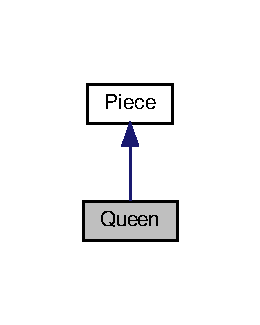
\includegraphics[width=125pt]{class_queen__inherit__graph}
\end{center}
\end{figure}


Collaboration diagram for Queen\+:\nopagebreak
\begin{figure}[H]
\begin{center}
\leavevmode
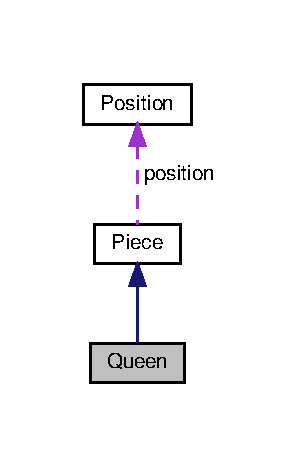
\includegraphics[width=143pt]{class_queen__coll__graph}
\end{center}
\end{figure}
\subsection*{Public Member Functions}
\begin{DoxyCompactItemize}
\item 
\hyperlink{class_queen_aa8675f82d1d05e7e457f94b897674ace}{Queen} (int \hyperlink{class_piece_aa8f39e11280395103164f6ae07398c82}{column}, int \hyperlink{class_piece_ac6ef7c474f20562cb629c2452ce0631d}{row}, \hyperlink{_piece_8h_ad7595c48bb74c0dd2a7648712a2d4985}{Piece\+Color} \hyperlink{class_piece_a8dfe0501fe95a1a7618cf5ad3b9fda69}{color})
\item 
std\+::vector$<$ \hyperlink{struct_position}{Position} $>$ \hyperlink{class_queen_a54461f7bace6797676679ad1da5901d3}{get\+Possible\+Moves} (std\+::shared\+\_\+ptr$<$ \hyperlink{class_base_board}{Base\+Board} $>$ board, bool initialboard) override
\item 
double \hyperlink{class_queen_aa2ca0d72a74a245470f502a82eaf1052}{get\+Position\+Value} () override
\end{DoxyCompactItemize}


\subsection{Constructor \& Destructor Documentation}
\mbox{\Hypertarget{class_queen_aa8675f82d1d05e7e457f94b897674ace}\label{class_queen_aa8675f82d1d05e7e457f94b897674ace}} 
\index{Queen@{Queen}!Queen@{Queen}}
\index{Queen@{Queen}!Queen@{Queen}}
\subsubsection{\texorpdfstring{Queen()}{Queen()}}
{\footnotesize\ttfamily Queen\+::\+Queen (\begin{DoxyParamCaption}\item[{int}]{column,  }\item[{int}]{row,  }\item[{\hyperlink{_piece_8h_ad7595c48bb74c0dd2a7648712a2d4985}{Piece\+Color}}]{color }\end{DoxyParamCaption})\hspace{0.3cm}{\ttfamily [inline]}}



\subsection{Member Function Documentation}
\mbox{\Hypertarget{class_queen_aa2ca0d72a74a245470f502a82eaf1052}\label{class_queen_aa2ca0d72a74a245470f502a82eaf1052}} 
\index{Queen@{Queen}!get\+Position\+Value@{get\+Position\+Value}}
\index{get\+Position\+Value@{get\+Position\+Value}!Queen@{Queen}}
\subsubsection{\texorpdfstring{get\+Position\+Value()}{getPositionValue()}}
{\footnotesize\ttfamily double Queen\+::get\+Position\+Value (\begin{DoxyParamCaption}{ }\end{DoxyParamCaption})\hspace{0.3cm}{\ttfamily [override]}, {\ttfamily [virtual]}}



Implements \hyperlink{class_piece_a4adfa58b4f0368c9a5859afcf294e0a4}{Piece}.

\mbox{\Hypertarget{class_queen_a54461f7bace6797676679ad1da5901d3}\label{class_queen_a54461f7bace6797676679ad1da5901d3}} 
\index{Queen@{Queen}!get\+Possible\+Moves@{get\+Possible\+Moves}}
\index{get\+Possible\+Moves@{get\+Possible\+Moves}!Queen@{Queen}}
\subsubsection{\texorpdfstring{get\+Possible\+Moves()}{getPossibleMoves()}}
{\footnotesize\ttfamily std\+::vector$<$ \hyperlink{struct_position}{Position} $>$ Queen\+::get\+Possible\+Moves (\begin{DoxyParamCaption}\item[{std\+::shared\+\_\+ptr$<$ \hyperlink{class_base_board}{Base\+Board} $>$}]{board,  }\item[{bool}]{initialboard }\end{DoxyParamCaption})\hspace{0.3cm}{\ttfamily [override]}, {\ttfamily [virtual]}}



Implements \hyperlink{class_piece_a8891924c280568529878549f59541925}{Piece}.



The documentation for this class was generated from the following files\+:\begin{DoxyCompactItemize}
\item 
lib/\hyperlink{_queen_8h}{Queen.\+h}\item 
\hyperlink{_queen_8cc}{Queen.\+cc}\end{DoxyCompactItemize}

\hypertarget{class_rook}{}\section{Rook Class Reference}
\label{class_rook}\index{Rook@{Rook}}


{\ttfamily \#include $<$Rook.\+h$>$}



Inheritance diagram for Rook\+:\nopagebreak
\begin{figure}[H]
\begin{center}
\leavevmode
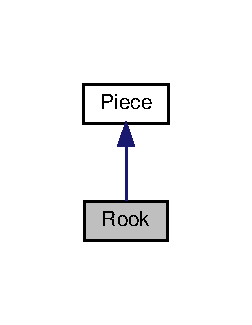
\includegraphics[width=121pt]{class_rook__inherit__graph}
\end{center}
\end{figure}


Collaboration diagram for Rook\+:\nopagebreak
\begin{figure}[H]
\begin{center}
\leavevmode
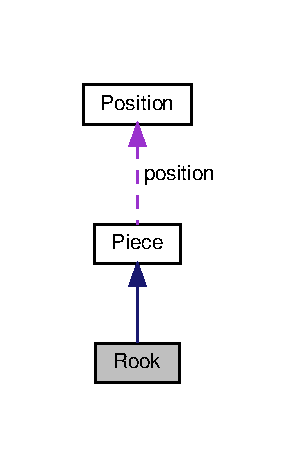
\includegraphics[width=143pt]{class_rook__coll__graph}
\end{center}
\end{figure}
\subsection*{Public Member Functions}
\begin{DoxyCompactItemize}
\item 
\hyperlink{class_rook_a757e308feb1c2d2635e8beb6d9b23369}{Rook} (int \hyperlink{class_piece_aa8f39e11280395103164f6ae07398c82}{column}, int \hyperlink{class_piece_ac6ef7c474f20562cb629c2452ce0631d}{row}, \hyperlink{_piece_8h_ad7595c48bb74c0dd2a7648712a2d4985}{Piece\+Color} \hyperlink{class_piece_a8dfe0501fe95a1a7618cf5ad3b9fda69}{color}, std\+::string \hyperlink{class_piece_af2fe809fd0d35d167f2419768e49fd3a}{figure\+Name})
\item 
std\+::vector$<$ \hyperlink{struct_position}{Position} $>$ \hyperlink{class_rook_ab186037a1f596102d618c1c9df31490d}{get\+Possible\+Moves} (std\+::shared\+\_\+ptr$<$ \hyperlink{class_base_board}{Base\+Board} $>$, bool) override
\item 
double \hyperlink{class_rook_ab1d83e6acb838249647f1f5fa7d17f41}{get\+Position\+Value} () override
\item 
bool \hyperlink{class_rook_a63c6d35a7f51e24d17079c80980dd948}{get\+Moved} ()
\item 
void \hyperlink{class_rook_a3ce8295607d89754d8c4be1813bc7b70}{set\+Moved} (bool)
\end{DoxyCompactItemize}
\subsection*{Private Attributes}
\begin{DoxyCompactItemize}
\item 
bool \hyperlink{class_rook_a2066de8a5df66bf3b8089d9d33e079ab}{moved} = false
\end{DoxyCompactItemize}


\subsection{Constructor \& Destructor Documentation}
\mbox{\Hypertarget{class_rook_a757e308feb1c2d2635e8beb6d9b23369}\label{class_rook_a757e308feb1c2d2635e8beb6d9b23369}} 
\index{Rook@{Rook}!Rook@{Rook}}
\index{Rook@{Rook}!Rook@{Rook}}
\subsubsection{\texorpdfstring{Rook()}{Rook()}}
{\footnotesize\ttfamily Rook\+::\+Rook (\begin{DoxyParamCaption}\item[{int}]{column,  }\item[{int}]{row,  }\item[{\hyperlink{_piece_8h_ad7595c48bb74c0dd2a7648712a2d4985}{Piece\+Color}}]{color,  }\item[{std\+::string}]{figure\+Name }\end{DoxyParamCaption})\hspace{0.3cm}{\ttfamily [inline]}}



\subsection{Member Function Documentation}
\mbox{\Hypertarget{class_rook_a63c6d35a7f51e24d17079c80980dd948}\label{class_rook_a63c6d35a7f51e24d17079c80980dd948}} 
\index{Rook@{Rook}!get\+Moved@{get\+Moved}}
\index{get\+Moved@{get\+Moved}!Rook@{Rook}}
\subsubsection{\texorpdfstring{get\+Moved()}{getMoved()}}
{\footnotesize\ttfamily bool Rook\+::get\+Moved (\begin{DoxyParamCaption}{ }\end{DoxyParamCaption})}

\mbox{\Hypertarget{class_rook_ab1d83e6acb838249647f1f5fa7d17f41}\label{class_rook_ab1d83e6acb838249647f1f5fa7d17f41}} 
\index{Rook@{Rook}!get\+Position\+Value@{get\+Position\+Value}}
\index{get\+Position\+Value@{get\+Position\+Value}!Rook@{Rook}}
\subsubsection{\texorpdfstring{get\+Position\+Value()}{getPositionValue()}}
{\footnotesize\ttfamily double Rook\+::get\+Position\+Value (\begin{DoxyParamCaption}{ }\end{DoxyParamCaption})\hspace{0.3cm}{\ttfamily [override]}, {\ttfamily [virtual]}}



Implements \hyperlink{class_piece_a4adfa58b4f0368c9a5859afcf294e0a4}{Piece}.

\mbox{\Hypertarget{class_rook_ab186037a1f596102d618c1c9df31490d}\label{class_rook_ab186037a1f596102d618c1c9df31490d}} 
\index{Rook@{Rook}!get\+Possible\+Moves@{get\+Possible\+Moves}}
\index{get\+Possible\+Moves@{get\+Possible\+Moves}!Rook@{Rook}}
\subsubsection{\texorpdfstring{get\+Possible\+Moves()}{getPossibleMoves()}}
{\footnotesize\ttfamily std\+::vector$<$ \hyperlink{struct_position}{Position} $>$ Rook\+::get\+Possible\+Moves (\begin{DoxyParamCaption}\item[{std\+::shared\+\_\+ptr$<$ \hyperlink{class_base_board}{Base\+Board} $>$}]{board,  }\item[{bool}]{original\+Evaluation }\end{DoxyParamCaption})\hspace{0.3cm}{\ttfamily [override]}, {\ttfamily [virtual]}}



Implements \hyperlink{class_piece_a8891924c280568529878549f59541925}{Piece}.

\mbox{\Hypertarget{class_rook_a3ce8295607d89754d8c4be1813bc7b70}\label{class_rook_a3ce8295607d89754d8c4be1813bc7b70}} 
\index{Rook@{Rook}!set\+Moved@{set\+Moved}}
\index{set\+Moved@{set\+Moved}!Rook@{Rook}}
\subsubsection{\texorpdfstring{set\+Moved()}{setMoved()}}
{\footnotesize\ttfamily void Rook\+::set\+Moved (\begin{DoxyParamCaption}\item[{bool}]{moved }\end{DoxyParamCaption})}



\subsection{Member Data Documentation}
\mbox{\Hypertarget{class_rook_a2066de8a5df66bf3b8089d9d33e079ab}\label{class_rook_a2066de8a5df66bf3b8089d9d33e079ab}} 
\index{Rook@{Rook}!moved@{moved}}
\index{moved@{moved}!Rook@{Rook}}
\subsubsection{\texorpdfstring{moved}{moved}}
{\footnotesize\ttfamily bool Rook\+::moved = false\hspace{0.3cm}{\ttfamily [private]}}



The documentation for this class was generated from the following files\+:\begin{DoxyCompactItemize}
\item 
lib/\hyperlink{_rook_8h}{Rook.\+h}\item 
\hyperlink{_rook_8cc}{Rook.\+cc}\end{DoxyCompactItemize}

\hypertarget{class_square}{}\section{Square Class Reference}
\label{class_square}\index{Square@{Square}}


{\ttfamily \#include $<$Square.\+h$>$}

\subsection*{Public Member Functions}
\begin{DoxyCompactItemize}
\item 
\hyperlink{class_square_abddcf314d0cf5edc08cadc7a73c8e590}{Square} (std\+::shared\+\_\+ptr$<$ \hyperlink{class_piece}{Piece} $>$)
\item 
void \hyperlink{class_square_a2daa860568eaf04bb8bdde747e0c929e}{set\+Piece} (std\+::shared\+\_\+ptr$<$ \hyperlink{class_piece}{Piece} $>$)
\item 
void \hyperlink{class_square_a759f5441bdd5499b33658c00c2179556}{set\+Column} (int)
\item 
void \hyperlink{class_square_a7efdf354c2f71ae95520162743efe170}{set\+Row} (int)
\item 
std\+::shared\+\_\+ptr$<$ \hyperlink{class_piece}{Piece} $>$ \hyperlink{class_square_add0bae19dd068f4ac9a5a3c54e0e088e}{get\+Piece} ()
\item 
int \hyperlink{class_square_ad3391313a44cdbfbe87fd3ddc545feac}{get\+Row} ()
\item 
int \hyperlink{class_square_a03943abf111f746327da0682babe8375}{get\+Column} ()
\item 
bool \hyperlink{class_square_a302ea5a61721ec621c5eac19766ff45f}{get\+Occupied} ()
\item 
void \hyperlink{class_square_a0a86c9e5d8d00ad8d33f4a8f11c0186d}{set\+Occupied} (bool)
\end{DoxyCompactItemize}
\subsection*{Private Attributes}
\begin{DoxyCompactItemize}
\item 
std\+::shared\+\_\+ptr$<$ \hyperlink{class_piece}{Piece} $>$ \hyperlink{class_square_aa3ea4ebade8191d5d1a1b23855b4e434}{piece} \{\}
\item 
int \hyperlink{class_square_a572fbccc549f148942d85208ce80605f}{column}
\item 
int \hyperlink{class_square_aa353950a9ef437401db55ae605b0f8b9}{row}
\item 
bool \hyperlink{class_square_ae6af3692dc17a771c296aacf2b40a99e}{occupied} = false
\end{DoxyCompactItemize}


\subsection{Constructor \& Destructor Documentation}
\mbox{\Hypertarget{class_square_abddcf314d0cf5edc08cadc7a73c8e590}\label{class_square_abddcf314d0cf5edc08cadc7a73c8e590}} 
\index{Square@{Square}!Square@{Square}}
\index{Square@{Square}!Square@{Square}}
\subsubsection{\texorpdfstring{Square()}{Square()}}
{\footnotesize\ttfamily Square\+::\+Square (\begin{DoxyParamCaption}\item[{std\+::shared\+\_\+ptr$<$ \hyperlink{class_piece}{Piece} $>$}]{piece }\end{DoxyParamCaption})}



\subsection{Member Function Documentation}
\mbox{\Hypertarget{class_square_a03943abf111f746327da0682babe8375}\label{class_square_a03943abf111f746327da0682babe8375}} 
\index{Square@{Square}!get\+Column@{get\+Column}}
\index{get\+Column@{get\+Column}!Square@{Square}}
\subsubsection{\texorpdfstring{get\+Column()}{getColumn()}}
{\footnotesize\ttfamily int Square\+::get\+Column (\begin{DoxyParamCaption}{ }\end{DoxyParamCaption})}

\mbox{\Hypertarget{class_square_a302ea5a61721ec621c5eac19766ff45f}\label{class_square_a302ea5a61721ec621c5eac19766ff45f}} 
\index{Square@{Square}!get\+Occupied@{get\+Occupied}}
\index{get\+Occupied@{get\+Occupied}!Square@{Square}}
\subsubsection{\texorpdfstring{get\+Occupied()}{getOccupied()}}
{\footnotesize\ttfamily bool Square\+::get\+Occupied (\begin{DoxyParamCaption}{ }\end{DoxyParamCaption})}

\mbox{\Hypertarget{class_square_add0bae19dd068f4ac9a5a3c54e0e088e}\label{class_square_add0bae19dd068f4ac9a5a3c54e0e088e}} 
\index{Square@{Square}!get\+Piece@{get\+Piece}}
\index{get\+Piece@{get\+Piece}!Square@{Square}}
\subsubsection{\texorpdfstring{get\+Piece()}{getPiece()}}
{\footnotesize\ttfamily std\+::shared\+\_\+ptr$<$ \hyperlink{class_piece}{Piece} $>$ Square\+::get\+Piece (\begin{DoxyParamCaption}{ }\end{DoxyParamCaption})}

\mbox{\Hypertarget{class_square_ad3391313a44cdbfbe87fd3ddc545feac}\label{class_square_ad3391313a44cdbfbe87fd3ddc545feac}} 
\index{Square@{Square}!get\+Row@{get\+Row}}
\index{get\+Row@{get\+Row}!Square@{Square}}
\subsubsection{\texorpdfstring{get\+Row()}{getRow()}}
{\footnotesize\ttfamily int Square\+::get\+Row (\begin{DoxyParamCaption}{ }\end{DoxyParamCaption})}

\mbox{\Hypertarget{class_square_a759f5441bdd5499b33658c00c2179556}\label{class_square_a759f5441bdd5499b33658c00c2179556}} 
\index{Square@{Square}!set\+Column@{set\+Column}}
\index{set\+Column@{set\+Column}!Square@{Square}}
\subsubsection{\texorpdfstring{set\+Column()}{setColumn()}}
{\footnotesize\ttfamily void Square\+::set\+Column (\begin{DoxyParamCaption}\item[{int}]{column }\end{DoxyParamCaption})}

\mbox{\Hypertarget{class_square_a0a86c9e5d8d00ad8d33f4a8f11c0186d}\label{class_square_a0a86c9e5d8d00ad8d33f4a8f11c0186d}} 
\index{Square@{Square}!set\+Occupied@{set\+Occupied}}
\index{set\+Occupied@{set\+Occupied}!Square@{Square}}
\subsubsection{\texorpdfstring{set\+Occupied()}{setOccupied()}}
{\footnotesize\ttfamily void Square\+::set\+Occupied (\begin{DoxyParamCaption}\item[{bool}]{occupied }\end{DoxyParamCaption})}

\mbox{\Hypertarget{class_square_a2daa860568eaf04bb8bdde747e0c929e}\label{class_square_a2daa860568eaf04bb8bdde747e0c929e}} 
\index{Square@{Square}!set\+Piece@{set\+Piece}}
\index{set\+Piece@{set\+Piece}!Square@{Square}}
\subsubsection{\texorpdfstring{set\+Piece()}{setPiece()}}
{\footnotesize\ttfamily void Square\+::set\+Piece (\begin{DoxyParamCaption}\item[{std\+::shared\+\_\+ptr$<$ \hyperlink{class_piece}{Piece} $>$}]{piece }\end{DoxyParamCaption})}

\mbox{\Hypertarget{class_square_a7efdf354c2f71ae95520162743efe170}\label{class_square_a7efdf354c2f71ae95520162743efe170}} 
\index{Square@{Square}!set\+Row@{set\+Row}}
\index{set\+Row@{set\+Row}!Square@{Square}}
\subsubsection{\texorpdfstring{set\+Row()}{setRow()}}
{\footnotesize\ttfamily void Square\+::set\+Row (\begin{DoxyParamCaption}\item[{int}]{row }\end{DoxyParamCaption})}



\subsection{Member Data Documentation}
\mbox{\Hypertarget{class_square_a572fbccc549f148942d85208ce80605f}\label{class_square_a572fbccc549f148942d85208ce80605f}} 
\index{Square@{Square}!column@{column}}
\index{column@{column}!Square@{Square}}
\subsubsection{\texorpdfstring{column}{column}}
{\footnotesize\ttfamily int Square\+::column\hspace{0.3cm}{\ttfamily [private]}}

\mbox{\Hypertarget{class_square_ae6af3692dc17a771c296aacf2b40a99e}\label{class_square_ae6af3692dc17a771c296aacf2b40a99e}} 
\index{Square@{Square}!occupied@{occupied}}
\index{occupied@{occupied}!Square@{Square}}
\subsubsection{\texorpdfstring{occupied}{occupied}}
{\footnotesize\ttfamily bool Square\+::occupied = false\hspace{0.3cm}{\ttfamily [private]}}

\mbox{\Hypertarget{class_square_aa3ea4ebade8191d5d1a1b23855b4e434}\label{class_square_aa3ea4ebade8191d5d1a1b23855b4e434}} 
\index{Square@{Square}!piece@{piece}}
\index{piece@{piece}!Square@{Square}}
\subsubsection{\texorpdfstring{piece}{piece}}
{\footnotesize\ttfamily std\+::shared\+\_\+ptr$<$\hyperlink{class_piece}{Piece}$>$ Square\+::piece \{\}\hspace{0.3cm}{\ttfamily [private]}}

\mbox{\Hypertarget{class_square_aa353950a9ef437401db55ae605b0f8b9}\label{class_square_aa353950a9ef437401db55ae605b0f8b9}} 
\index{Square@{Square}!row@{row}}
\index{row@{row}!Square@{Square}}
\subsubsection{\texorpdfstring{row}{row}}
{\footnotesize\ttfamily int Square\+::row\hspace{0.3cm}{\ttfamily [private]}}



The documentation for this class was generated from the following files\+:\begin{DoxyCompactItemize}
\item 
lib/\hyperlink{_square_8h}{Square.\+h}\item 
\hyperlink{_square_8cc}{Square.\+cc}\end{DoxyCompactItemize}

\hypertarget{class_wrong_arg_exception}{}\section{Wrong\+Arg\+Exception Class Reference}
\label{class_wrong_arg_exception}\index{Wrong\+Arg\+Exception@{Wrong\+Arg\+Exception}}


{\ttfamily \#include $<$Wrong\+Arg\+Exception.\+h$>$}



Inheritance diagram for Wrong\+Arg\+Exception\+:\nopagebreak
\begin{figure}[H]
\begin{center}
\leavevmode
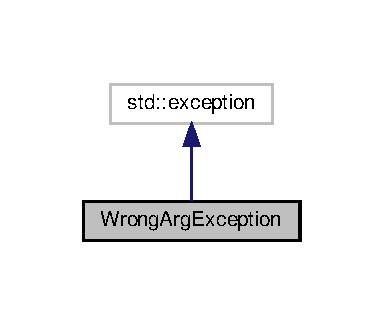
\includegraphics[width=184pt]{class_wrong_arg_exception__inherit__graph}
\end{center}
\end{figure}


Collaboration diagram for Wrong\+Arg\+Exception\+:\nopagebreak
\begin{figure}[H]
\begin{center}
\leavevmode
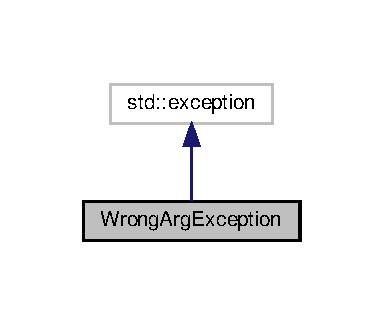
\includegraphics[width=184pt]{class_wrong_arg_exception__coll__graph}
\end{center}
\end{figure}
\subsection*{Public Member Functions}
\begin{DoxyCompactItemize}
\item 
\hyperlink{class_wrong_arg_exception_a9462f257043ca3fa9bace884a103b67e}{Wrong\+Arg\+Exception} (std\+::string \hyperlink{class_wrong_arg_exception_a8ed636869cba7a41440f63795fef9ede}{text})
\end{DoxyCompactItemize}
\subsection*{Private Attributes}
\begin{DoxyCompactItemize}
\item 
std\+::string \hyperlink{class_wrong_arg_exception_a8ed636869cba7a41440f63795fef9ede}{text}
\end{DoxyCompactItemize}


\subsection{Constructor \& Destructor Documentation}
\mbox{\Hypertarget{class_wrong_arg_exception_a9462f257043ca3fa9bace884a103b67e}\label{class_wrong_arg_exception_a9462f257043ca3fa9bace884a103b67e}} 
\index{Wrong\+Arg\+Exception@{Wrong\+Arg\+Exception}!Wrong\+Arg\+Exception@{Wrong\+Arg\+Exception}}
\index{Wrong\+Arg\+Exception@{Wrong\+Arg\+Exception}!Wrong\+Arg\+Exception@{Wrong\+Arg\+Exception}}
\subsubsection{\texorpdfstring{Wrong\+Arg\+Exception()}{WrongArgException()}}
{\footnotesize\ttfamily Wrong\+Arg\+Exception\+::\+Wrong\+Arg\+Exception (\begin{DoxyParamCaption}\item[{std\+::string}]{text }\end{DoxyParamCaption})}



\subsection{Member Data Documentation}
\mbox{\Hypertarget{class_wrong_arg_exception_a8ed636869cba7a41440f63795fef9ede}\label{class_wrong_arg_exception_a8ed636869cba7a41440f63795fef9ede}} 
\index{Wrong\+Arg\+Exception@{Wrong\+Arg\+Exception}!text@{text}}
\index{text@{text}!Wrong\+Arg\+Exception@{Wrong\+Arg\+Exception}}
\subsubsection{\texorpdfstring{text}{text}}
{\footnotesize\ttfamily std\+::string Wrong\+Arg\+Exception\+::text\hspace{0.3cm}{\ttfamily [private]}}



The documentation for this class was generated from the following files\+:\begin{DoxyCompactItemize}
\item 
exceptions/\hyperlink{_wrong_arg_exception_8h}{Wrong\+Arg\+Exception.\+h}\item 
exceptions/\hyperlink{_wrong_arg_exception_8cpp}{Wrong\+Arg\+Exception.\+cpp}\end{DoxyCompactItemize}

\chapter{File Documentation}
\hypertarget{_a_i_class_8cpp}{}\section{A\+I/\+A\+I\+Class.cpp File Reference}
\label{_a_i_class_8cpp}\index{A\+I/\+A\+I\+Class.\+cpp@{A\+I/\+A\+I\+Class.\+cpp}}
{\ttfamily \#include \char`\"{}A\+I\+Class.\+h\char`\"{}}\newline
{\ttfamily \#include \char`\"{}../lib/\+Base\+Board.\+h\char`\"{}}\newline
Include dependency graph for A\+I\+Class.\+cpp\+:\nopagebreak
\begin{figure}[H]
\begin{center}
\leavevmode
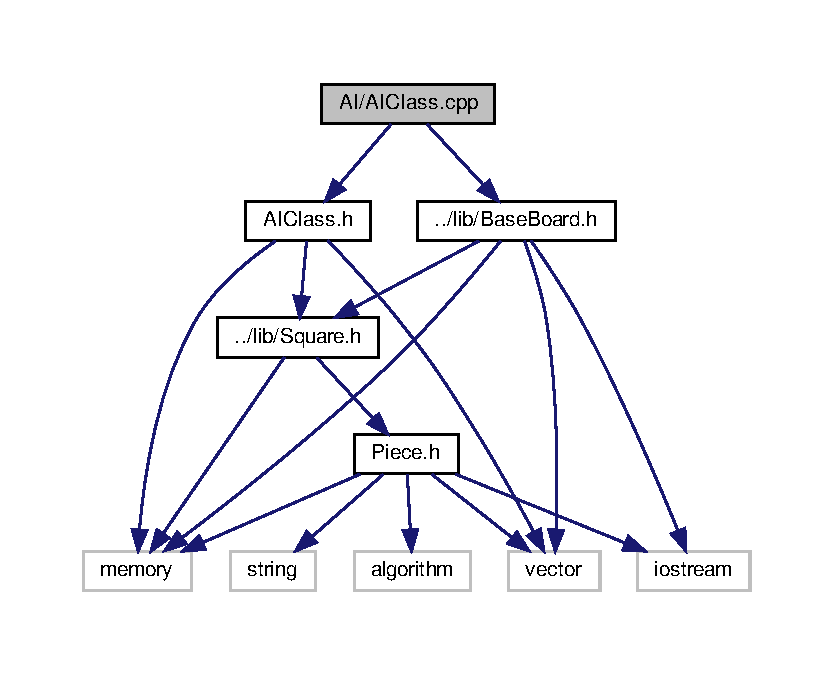
\includegraphics[width=350pt]{_a_i_class_8cpp__incl}
\end{center}
\end{figure}

\hypertarget{_a_i_class_8h}{}\section{A\+I/\+A\+I\+Class.h File Reference}
\label{_a_i_class_8h}\index{A\+I/\+A\+I\+Class.\+h@{A\+I/\+A\+I\+Class.\+h}}
{\ttfamily \#include $<$memory$>$}\newline
{\ttfamily \#include $<$vector$>$}\newline
{\ttfamily \#include \char`\"{}../lib/\+Square.\+h\char`\"{}}\newline
Include dependency graph for A\+I\+Class.\+h\+:\nopagebreak
\begin{figure}[H]
\begin{center}
\leavevmode
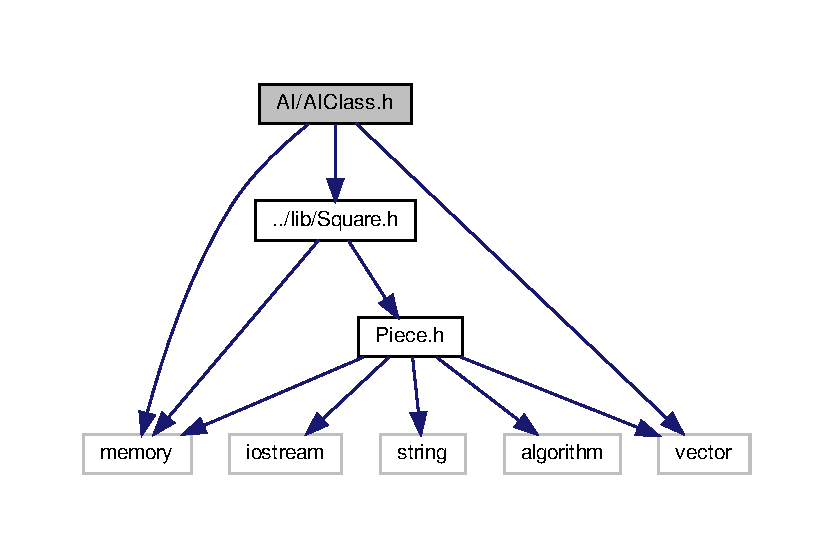
\includegraphics[width=350pt]{_a_i_class_8h__incl}
\end{center}
\end{figure}
This graph shows which files directly or indirectly include this file\+:\nopagebreak
\begin{figure}[H]
\begin{center}
\leavevmode
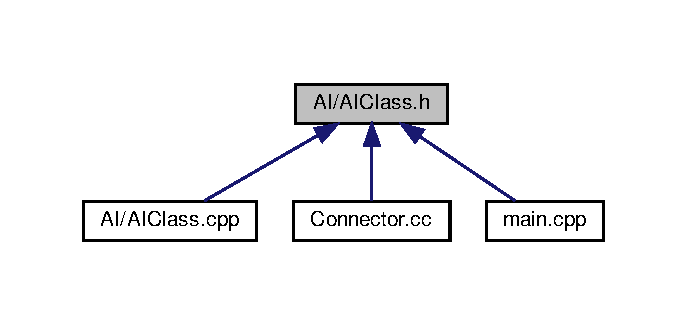
\includegraphics[width=330pt]{_a_i_class_8h__dep__incl}
\end{center}
\end{figure}
\subsection*{Classes}
\begin{DoxyCompactItemize}
\item 
struct \hyperlink{struct_move_packet}{Move\+Packet}
\item 
class \hyperlink{class_a_i_class}{A\+I\+Class}
\end{DoxyCompactItemize}
\subsection*{Typedefs}
\begin{DoxyCompactItemize}
\item 
typedef std\+::vector$<$ std\+::vector$<$ std\+::shared\+\_\+ptr$<$ \hyperlink{class_square}{Square} $>$ $>$ $>$ \hyperlink{_a_i_class_8h_a6e73002e9c84a7986c39d7e80e83dc8d}{board\+\_\+type}
\end{DoxyCompactItemize}


\subsection{Typedef Documentation}
\mbox{\Hypertarget{_a_i_class_8h_a6e73002e9c84a7986c39d7e80e83dc8d}\label{_a_i_class_8h_a6e73002e9c84a7986c39d7e80e83dc8d}} 
\index{A\+I\+Class.\+h@{A\+I\+Class.\+h}!board\+\_\+type@{board\+\_\+type}}
\index{board\+\_\+type@{board\+\_\+type}!A\+I\+Class.\+h@{A\+I\+Class.\+h}}
\subsubsection{\texorpdfstring{board\+\_\+type}{board\_type}}
{\footnotesize\ttfamily typedef std\+::vector$<$std\+::vector $<$std\+::shared\+\_\+ptr$<$\hyperlink{class_square}{Square}$>$ $>$ $>$ \hyperlink{_a_i_class_8h_a6e73002e9c84a7986c39d7e80e83dc8d}{board\+\_\+type}}


\hypertarget{_position_value_8cpp}{}\section{A\+I/\+Position\+Value.cpp File Reference}
\label{_position_value_8cpp}\index{A\+I/\+Position\+Value.\+cpp@{A\+I/\+Position\+Value.\+cpp}}
{\ttfamily \#include \char`\"{}Position\+Value.\+h\char`\"{}}\newline
Include dependency graph for Position\+Value.\+cpp\+:\nopagebreak
\begin{figure}[H]
\begin{center}
\leavevmode
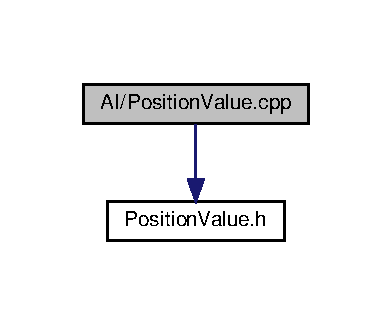
\includegraphics[width=188pt]{_position_value_8cpp__incl}
\end{center}
\end{figure}

\hypertarget{_position_value_8h}{}\section{A\+I/\+Position\+Value.h File Reference}
\label{_position_value_8h}\index{A\+I/\+Position\+Value.\+h@{A\+I/\+Position\+Value.\+h}}
This graph shows which files directly or indirectly include this file\+:\nopagebreak
\begin{figure}[H]
\begin{center}
\leavevmode
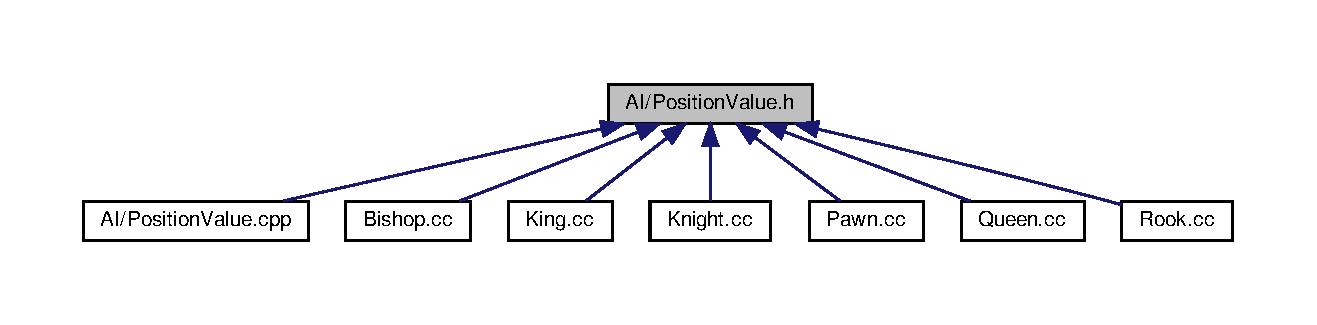
\includegraphics[width=350pt]{_position_value_8h__dep__incl}
\end{center}
\end{figure}
\subsection*{Classes}
\begin{DoxyCompactItemize}
\item 
class \hyperlink{class_position_value}{Position\+Value}
\end{DoxyCompactItemize}

\hypertarget{_base_board_8cc}{}\section{Base\+Board.\+cc File Reference}
\label{_base_board_8cc}\index{Base\+Board.\+cc@{Base\+Board.\+cc}}
{\ttfamily \#include \char`\"{}lib/\+Base\+Board.\+h\char`\"{}}\newline
{\ttfamily \#include $<$memory$>$}\newline
{\ttfamily \#include \char`\"{}lib/\+Piece.\+h\char`\"{}}\newline
{\ttfamily \#include \char`\"{}lib/\+Bishop.\+h\char`\"{}}\newline
{\ttfamily \#include \char`\"{}lib/\+Rook.\+h\char`\"{}}\newline
{\ttfamily \#include \char`\"{}lib/\+Knight.\+h\char`\"{}}\newline
{\ttfamily \#include \char`\"{}lib/\+King.\+h\char`\"{}}\newline
{\ttfamily \#include \char`\"{}lib/\+Queen.\+h\char`\"{}}\newline
{\ttfamily \#include \char`\"{}lib/\+Pawn.\+h\char`\"{}}\newline
Include dependency graph for Base\+Board.\+cc\+:
\nopagebreak
\begin{figure}[H]
\begin{center}
\leavevmode
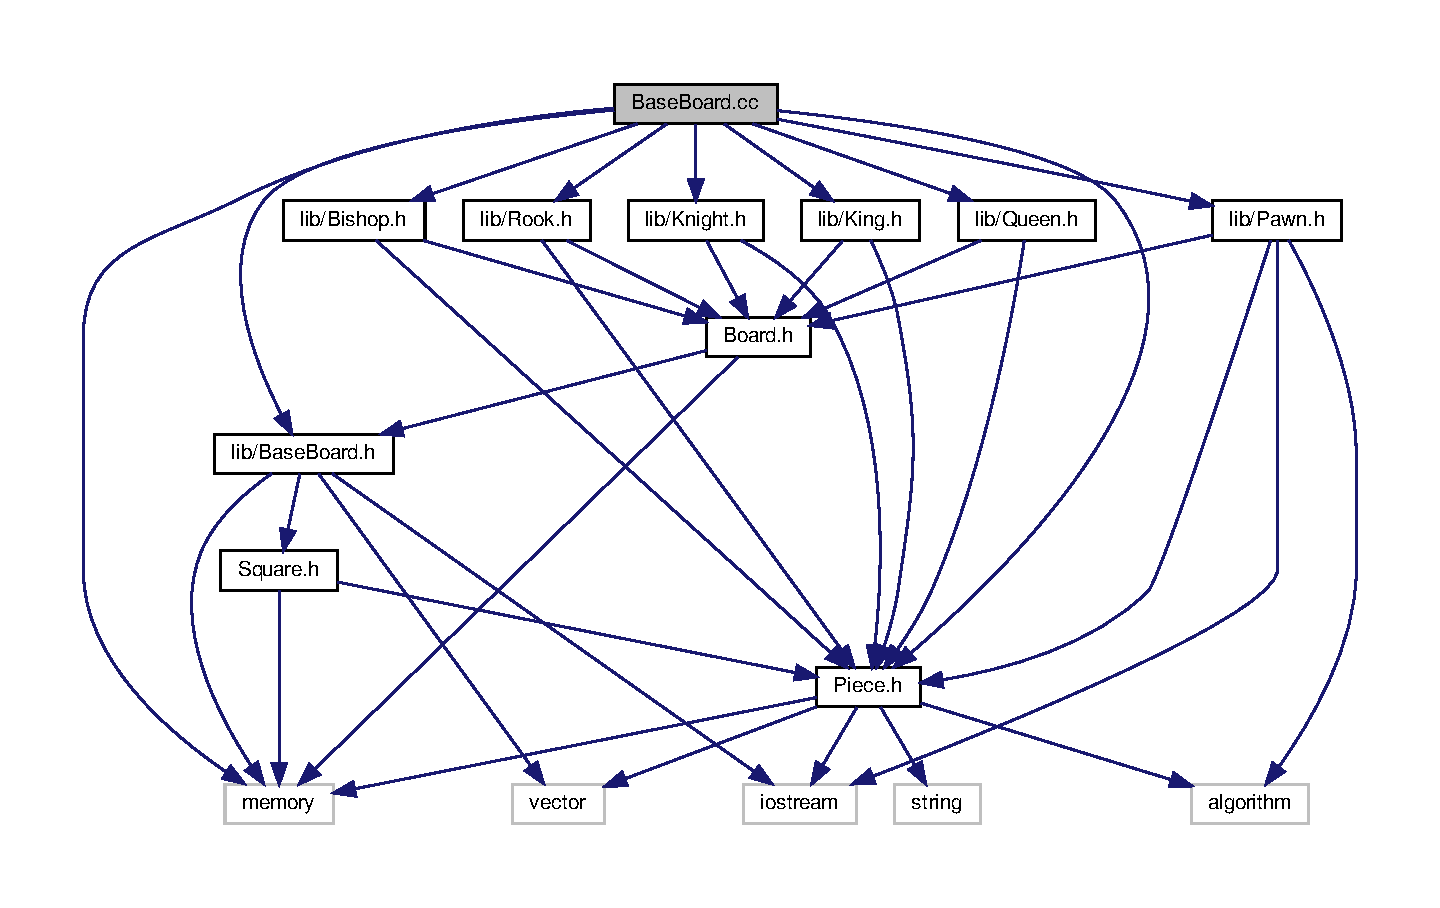
\includegraphics[width=350pt]{_base_board_8cc__incl}
\end{center}
\end{figure}
\subsection*{Variables}
\begin{DoxyCompactItemize}
\item 
std\+::vector$<$ std\+::vector$<$ std\+::string $>$ $>$ const \hyperlink{_base_board_8cc_a9965e03c4f48ae012bf1d93c397bf22c}{I\+N\+I\+T\+I\+A\+L\+\_\+\+B\+O\+A\+RD}
\begin{DoxyCompactList}\small\item\em vector used to initialize starting boards \end{DoxyCompactList}\end{DoxyCompactItemize}


\subsection{Variable Documentation}
\mbox{\Hypertarget{_base_board_8cc_a9965e03c4f48ae012bf1d93c397bf22c}\label{_base_board_8cc_a9965e03c4f48ae012bf1d93c397bf22c}} 
\index{Base\+Board.\+cc@{Base\+Board.\+cc}!I\+N\+I\+T\+I\+A\+L\+\_\+\+B\+O\+A\+RD@{I\+N\+I\+T\+I\+A\+L\+\_\+\+B\+O\+A\+RD}}
\index{I\+N\+I\+T\+I\+A\+L\+\_\+\+B\+O\+A\+RD@{I\+N\+I\+T\+I\+A\+L\+\_\+\+B\+O\+A\+RD}!Base\+Board.\+cc@{Base\+Board.\+cc}}
\subsubsection{\texorpdfstring{I\+N\+I\+T\+I\+A\+L\+\_\+\+B\+O\+A\+RD}{INITIAL\_BOARD}}
{\footnotesize\ttfamily std\+::vector$<$std\+::vector $<$std\+::string$>$ $>$ const I\+N\+I\+T\+I\+A\+L\+\_\+\+B\+O\+A\+RD}



vector used to initialize starting boards 


\hypertarget{_bishop_8cc}{}\section{Bishop.\+cc File Reference}
\label{_bishop_8cc}\index{Bishop.\+cc@{Bishop.\+cc}}
{\ttfamily \#include \char`\"{}A\+I/\+Position\+Value.\+h\char`\"{}}\newline
{\ttfamily \#include \char`\"{}lib/\+Bishop.\+h\char`\"{}}\newline
Include dependency graph for Bishop.\+cc\+:\nopagebreak
\begin{figure}[H]
\begin{center}
\leavevmode
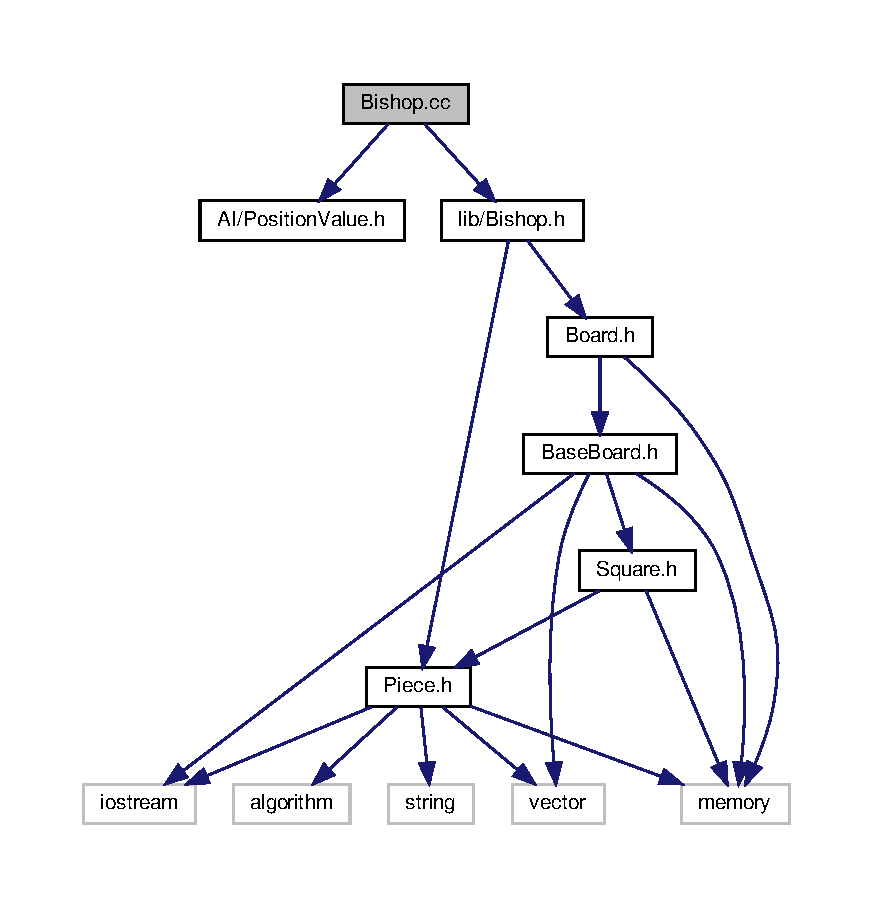
\includegraphics[width=350pt]{_bishop_8cc__incl}
\end{center}
\end{figure}

\hypertarget{_board_8cc}{}\section{Board.\+cc File Reference}
\label{_board_8cc}\index{Board.\+cc@{Board.\+cc}}
{\ttfamily \#include \char`\"{}lib/\+Base\+Board.\+h\char`\"{}}\newline
{\ttfamily \#include \char`\"{}lib/\+Board.\+h\char`\"{}}\newline
{\ttfamily \#include $<$iostream$>$}\newline
{\ttfamily \#include $<$memory$>$}\newline
Include dependency graph for Board.\+cc\+:\nopagebreak
\begin{figure}[H]
\begin{center}
\leavevmode
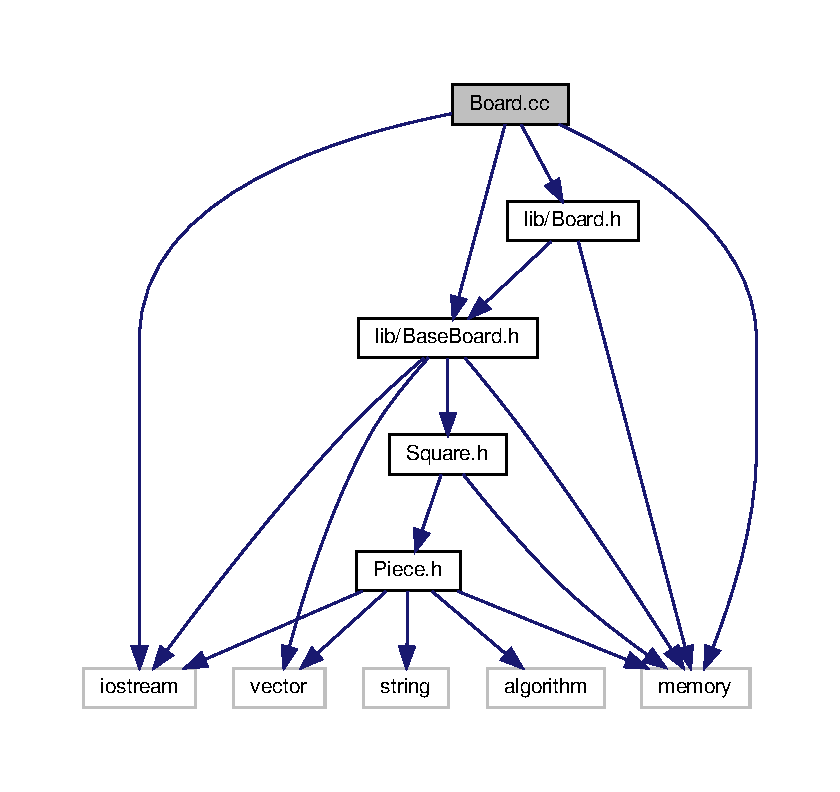
\includegraphics[width=350pt]{_board_8cc__incl}
\end{center}
\end{figure}

\hypertarget{_c_make_files_23_810_82_2_compiler_id_c_2_c_make_c_compiler_id_8c}{}\section{C\+Make\+Files/3.10.2/\+Compiler\+Id\+C/\+C\+Make\+C\+Compiler\+Id.c File Reference}
\label{_c_make_files_23_810_82_2_compiler_id_c_2_c_make_c_compiler_id_8c}\index{C\+Make\+Files/3.\+10.\+2/\+Compiler\+Id\+C/\+C\+Make\+C\+Compiler\+Id.\+c@{C\+Make\+Files/3.\+10.\+2/\+Compiler\+Id\+C/\+C\+Make\+C\+Compiler\+Id.\+c}}
\subsection*{Macros}
\begin{DoxyCompactItemize}
\item 
\#define \hyperlink{_c_make_files_23_810_82_2_compiler_id_c_2_c_make_c_compiler_id_8c_a81dee0709ded976b2e0319239f72d174}{C\+O\+M\+P\+I\+L\+E\+R\+\_\+\+ID}~\char`\"{}\char`\"{}
\item 
\#define \hyperlink{_c_make_files_23_810_82_2_compiler_id_c_2_c_make_c_compiler_id_8c_a2ae9b72bb13abaabfcf2ee0ba7d3fa1d}{S\+T\+R\+I\+N\+G\+I\+F\+Y\+\_\+\+H\+E\+L\+P\+ER}(X)~\#X
\item 
\#define \hyperlink{_c_make_files_23_810_82_2_compiler_id_c_2_c_make_c_compiler_id_8c_a43e1cad902b6477bec893cb6430bd6c8}{S\+T\+R\+I\+N\+G\+I\+FY}(X)~\hyperlink{test_2_c_make_files_23_810_82_2_compiler_id_c_x_x_2_c_make_c_x_x_compiler_id_8cpp_a2ae9b72bb13abaabfcf2ee0ba7d3fa1d}{S\+T\+R\+I\+N\+G\+I\+F\+Y\+\_\+\+H\+E\+L\+P\+ER}(X)
\item 
\#define \hyperlink{_c_make_files_23_810_82_2_compiler_id_c_2_c_make_c_compiler_id_8c_adbc5372f40838899018fadbc89bd588b}{P\+L\+A\+T\+F\+O\+R\+M\+\_\+\+ID}
\item 
\#define \hyperlink{_c_make_files_23_810_82_2_compiler_id_c_2_c_make_c_compiler_id_8c_aba35d0d200deaeb06aee95ca297acb28}{A\+R\+C\+H\+I\+T\+E\+C\+T\+U\+R\+E\+\_\+\+ID}
\item 
\#define \hyperlink{_c_make_files_23_810_82_2_compiler_id_c_2_c_make_c_compiler_id_8c_ad1280362da42492bbc11aa78cbf776ad}{D\+EC}(n)
\item 
\#define \hyperlink{_c_make_files_23_810_82_2_compiler_id_c_2_c_make_c_compiler_id_8c_a46d5d95daa1bef867bd0179594310ed5}{H\+EX}(n)
\item 
\#define \hyperlink{_c_make_files_23_810_82_2_compiler_id_c_2_c_make_c_compiler_id_8c_a07f8e5783674099cd7f5110e22a78cdb}{C\+\_\+\+D\+I\+A\+L\+E\+CT}
\end{DoxyCompactItemize}
\subsection*{Functions}
\begin{DoxyCompactItemize}
\item 
int \hyperlink{_c_make_files_23_810_82_2_compiler_id_c_2_c_make_c_compiler_id_8c_a0ddf1224851353fc92bfbff6f499fa97}{main} (int argc, char $\ast$argv\mbox{[}$\,$\mbox{]})
\end{DoxyCompactItemize}
\subsection*{Variables}
\begin{DoxyCompactItemize}
\item 
char const  $\ast$ \hyperlink{_c_make_files_23_810_82_2_compiler_id_c_2_c_make_c_compiler_id_8c_a4b0efeb7a5d59313986b3a0390f050f6}{info\+\_\+compiler} = \char`\"{}I\+N\+FO\char`\"{} \char`\"{}\+:\char`\"{} \char`\"{}compiler\mbox{[}\char`\"{} C\+O\+M\+P\+I\+L\+E\+R\+\_\+\+ID \char`\"{}\mbox{]}\char`\"{}
\item 
char const  $\ast$ \hyperlink{_c_make_files_23_810_82_2_compiler_id_c_2_c_make_c_compiler_id_8c_a2321403dee54ee23f0c2fa849c60f7d4}{info\+\_\+platform} = \char`\"{}I\+N\+FO\char`\"{} \char`\"{}\+:\char`\"{} \char`\"{}platform\mbox{[}\char`\"{} P\+L\+A\+T\+F\+O\+R\+M\+\_\+\+ID \char`\"{}\mbox{]}\char`\"{}
\item 
char const  $\ast$ \hyperlink{_c_make_files_23_810_82_2_compiler_id_c_2_c_make_c_compiler_id_8c_a59647e99d304ed33b15cb284c27ed391}{info\+\_\+arch} = \char`\"{}I\+N\+FO\char`\"{} \char`\"{}\+:\char`\"{} \char`\"{}arch\mbox{[}\char`\"{} A\+R\+C\+H\+I\+T\+E\+C\+T\+U\+R\+E\+\_\+\+ID \char`\"{}\mbox{]}\char`\"{}
\item 
const char $\ast$ \hyperlink{_c_make_files_23_810_82_2_compiler_id_c_2_c_make_c_compiler_id_8c_a1ce162bad2fe6966ac8b33cc19e120b8}{info\+\_\+language\+\_\+dialect\+\_\+default}
\end{DoxyCompactItemize}


\subsection{Macro Definition Documentation}
\mbox{\Hypertarget{_c_make_files_23_810_82_2_compiler_id_c_2_c_make_c_compiler_id_8c_aba35d0d200deaeb06aee95ca297acb28}\label{_c_make_files_23_810_82_2_compiler_id_c_2_c_make_c_compiler_id_8c_aba35d0d200deaeb06aee95ca297acb28}} 
\index{C\+Make\+Files/3.\+10.\+2/\+Compiler\+Id\+C/\+C\+Make\+C\+Compiler\+Id.\+c@{C\+Make\+Files/3.\+10.\+2/\+Compiler\+Id\+C/\+C\+Make\+C\+Compiler\+Id.\+c}!A\+R\+C\+H\+I\+T\+E\+C\+T\+U\+R\+E\+\_\+\+ID@{A\+R\+C\+H\+I\+T\+E\+C\+T\+U\+R\+E\+\_\+\+ID}}
\index{A\+R\+C\+H\+I\+T\+E\+C\+T\+U\+R\+E\+\_\+\+ID@{A\+R\+C\+H\+I\+T\+E\+C\+T\+U\+R\+E\+\_\+\+ID}!C\+Make\+Files/3.\+10.\+2/\+Compiler\+Id\+C/\+C\+Make\+C\+Compiler\+Id.\+c@{C\+Make\+Files/3.\+10.\+2/\+Compiler\+Id\+C/\+C\+Make\+C\+Compiler\+Id.\+c}}
\subsubsection{\texorpdfstring{A\+R\+C\+H\+I\+T\+E\+C\+T\+U\+R\+E\+\_\+\+ID}{ARCHITECTURE\_ID}}
{\footnotesize\ttfamily \#define A\+R\+C\+H\+I\+T\+E\+C\+T\+U\+R\+E\+\_\+\+ID}

\mbox{\Hypertarget{_c_make_files_23_810_82_2_compiler_id_c_2_c_make_c_compiler_id_8c_a07f8e5783674099cd7f5110e22a78cdb}\label{_c_make_files_23_810_82_2_compiler_id_c_2_c_make_c_compiler_id_8c_a07f8e5783674099cd7f5110e22a78cdb}} 
\index{C\+Make\+Files/3.\+10.\+2/\+Compiler\+Id\+C/\+C\+Make\+C\+Compiler\+Id.\+c@{C\+Make\+Files/3.\+10.\+2/\+Compiler\+Id\+C/\+C\+Make\+C\+Compiler\+Id.\+c}!C\+\_\+\+D\+I\+A\+L\+E\+CT@{C\+\_\+\+D\+I\+A\+L\+E\+CT}}
\index{C\+\_\+\+D\+I\+A\+L\+E\+CT@{C\+\_\+\+D\+I\+A\+L\+E\+CT}!C\+Make\+Files/3.\+10.\+2/\+Compiler\+Id\+C/\+C\+Make\+C\+Compiler\+Id.\+c@{C\+Make\+Files/3.\+10.\+2/\+Compiler\+Id\+C/\+C\+Make\+C\+Compiler\+Id.\+c}}
\subsubsection{\texorpdfstring{C\+\_\+\+D\+I\+A\+L\+E\+CT}{C\_DIALECT}}
{\footnotesize\ttfamily \#define C\+\_\+\+D\+I\+A\+L\+E\+CT}

\mbox{\Hypertarget{_c_make_files_23_810_82_2_compiler_id_c_2_c_make_c_compiler_id_8c_a81dee0709ded976b2e0319239f72d174}\label{_c_make_files_23_810_82_2_compiler_id_c_2_c_make_c_compiler_id_8c_a81dee0709ded976b2e0319239f72d174}} 
\index{C\+Make\+Files/3.\+10.\+2/\+Compiler\+Id\+C/\+C\+Make\+C\+Compiler\+Id.\+c@{C\+Make\+Files/3.\+10.\+2/\+Compiler\+Id\+C/\+C\+Make\+C\+Compiler\+Id.\+c}!C\+O\+M\+P\+I\+L\+E\+R\+\_\+\+ID@{C\+O\+M\+P\+I\+L\+E\+R\+\_\+\+ID}}
\index{C\+O\+M\+P\+I\+L\+E\+R\+\_\+\+ID@{C\+O\+M\+P\+I\+L\+E\+R\+\_\+\+ID}!C\+Make\+Files/3.\+10.\+2/\+Compiler\+Id\+C/\+C\+Make\+C\+Compiler\+Id.\+c@{C\+Make\+Files/3.\+10.\+2/\+Compiler\+Id\+C/\+C\+Make\+C\+Compiler\+Id.\+c}}
\subsubsection{\texorpdfstring{C\+O\+M\+P\+I\+L\+E\+R\+\_\+\+ID}{COMPILER\_ID}}
{\footnotesize\ttfamily \#define C\+O\+M\+P\+I\+L\+E\+R\+\_\+\+ID~\char`\"{}\char`\"{}}

\mbox{\Hypertarget{_c_make_files_23_810_82_2_compiler_id_c_2_c_make_c_compiler_id_8c_ad1280362da42492bbc11aa78cbf776ad}\label{_c_make_files_23_810_82_2_compiler_id_c_2_c_make_c_compiler_id_8c_ad1280362da42492bbc11aa78cbf776ad}} 
\index{C\+Make\+Files/3.\+10.\+2/\+Compiler\+Id\+C/\+C\+Make\+C\+Compiler\+Id.\+c@{C\+Make\+Files/3.\+10.\+2/\+Compiler\+Id\+C/\+C\+Make\+C\+Compiler\+Id.\+c}!D\+EC@{D\+EC}}
\index{D\+EC@{D\+EC}!C\+Make\+Files/3.\+10.\+2/\+Compiler\+Id\+C/\+C\+Make\+C\+Compiler\+Id.\+c@{C\+Make\+Files/3.\+10.\+2/\+Compiler\+Id\+C/\+C\+Make\+C\+Compiler\+Id.\+c}}
\subsubsection{\texorpdfstring{D\+EC}{DEC}}
{\footnotesize\ttfamily \#define D\+EC(\begin{DoxyParamCaption}\item[{}]{n }\end{DoxyParamCaption})}

{\bfseries Value\+:}
\begin{DoxyCode}
(\textcolor{charliteral}{'0'} + (((n) / 10000000)%10)), \(\backslash\)
  (\textcolor{charliteral}{'0'} + (((n) / 1000000)%10)),  \(\backslash\)
  (\textcolor{charliteral}{'0'} + (((n) / 100000)%10)),   \(\backslash\)
  (\textcolor{charliteral}{'0'} + (((n) / 10000)%10)),    \(\backslash\)
  (\textcolor{charliteral}{'0'} + (((n) / 1000)%10)),     \(\backslash\)
  (\textcolor{charliteral}{'0'} + (((n) / 100)%10)),      \(\backslash\)
  (\textcolor{charliteral}{'0'} + (((n) / 10)%10)),       \(\backslash\)
  (\textcolor{charliteral}{'0'} +  ((n) % 10))
\end{DoxyCode}
\mbox{\Hypertarget{_c_make_files_23_810_82_2_compiler_id_c_2_c_make_c_compiler_id_8c_a46d5d95daa1bef867bd0179594310ed5}\label{_c_make_files_23_810_82_2_compiler_id_c_2_c_make_c_compiler_id_8c_a46d5d95daa1bef867bd0179594310ed5}} 
\index{C\+Make\+Files/3.\+10.\+2/\+Compiler\+Id\+C/\+C\+Make\+C\+Compiler\+Id.\+c@{C\+Make\+Files/3.\+10.\+2/\+Compiler\+Id\+C/\+C\+Make\+C\+Compiler\+Id.\+c}!H\+EX@{H\+EX}}
\index{H\+EX@{H\+EX}!C\+Make\+Files/3.\+10.\+2/\+Compiler\+Id\+C/\+C\+Make\+C\+Compiler\+Id.\+c@{C\+Make\+Files/3.\+10.\+2/\+Compiler\+Id\+C/\+C\+Make\+C\+Compiler\+Id.\+c}}
\subsubsection{\texorpdfstring{H\+EX}{HEX}}
{\footnotesize\ttfamily \#define H\+EX(\begin{DoxyParamCaption}\item[{}]{n }\end{DoxyParamCaption})}

{\bfseries Value\+:}
\begin{DoxyCode}
(\textcolor{charliteral}{'0'} + ((n)>>28 & 0xF)), \(\backslash\)
  (\textcolor{charliteral}{'0'} + ((n)>>24 & 0xF)), \(\backslash\)
  (\textcolor{charliteral}{'0'} + ((n)>>20 & 0xF)), \(\backslash\)
  (\textcolor{charliteral}{'0'} + ((n)>>16 & 0xF)), \(\backslash\)
  (\textcolor{charliteral}{'0'} + ((n)>>12 & 0xF)), \(\backslash\)
  (\textcolor{charliteral}{'0'} + ((n)>>8  & 0xF)), \(\backslash\)
  (\textcolor{charliteral}{'0'} + ((n)>>4  & 0xF)), \(\backslash\)
  (\textcolor{charliteral}{'0'} + ((n)     & 0xF))
\end{DoxyCode}
\mbox{\Hypertarget{_c_make_files_23_810_82_2_compiler_id_c_2_c_make_c_compiler_id_8c_adbc5372f40838899018fadbc89bd588b}\label{_c_make_files_23_810_82_2_compiler_id_c_2_c_make_c_compiler_id_8c_adbc5372f40838899018fadbc89bd588b}} 
\index{C\+Make\+Files/3.\+10.\+2/\+Compiler\+Id\+C/\+C\+Make\+C\+Compiler\+Id.\+c@{C\+Make\+Files/3.\+10.\+2/\+Compiler\+Id\+C/\+C\+Make\+C\+Compiler\+Id.\+c}!P\+L\+A\+T\+F\+O\+R\+M\+\_\+\+ID@{P\+L\+A\+T\+F\+O\+R\+M\+\_\+\+ID}}
\index{P\+L\+A\+T\+F\+O\+R\+M\+\_\+\+ID@{P\+L\+A\+T\+F\+O\+R\+M\+\_\+\+ID}!C\+Make\+Files/3.\+10.\+2/\+Compiler\+Id\+C/\+C\+Make\+C\+Compiler\+Id.\+c@{C\+Make\+Files/3.\+10.\+2/\+Compiler\+Id\+C/\+C\+Make\+C\+Compiler\+Id.\+c}}
\subsubsection{\texorpdfstring{P\+L\+A\+T\+F\+O\+R\+M\+\_\+\+ID}{PLATFORM\_ID}}
{\footnotesize\ttfamily \#define P\+L\+A\+T\+F\+O\+R\+M\+\_\+\+ID}

\mbox{\Hypertarget{_c_make_files_23_810_82_2_compiler_id_c_2_c_make_c_compiler_id_8c_a43e1cad902b6477bec893cb6430bd6c8}\label{_c_make_files_23_810_82_2_compiler_id_c_2_c_make_c_compiler_id_8c_a43e1cad902b6477bec893cb6430bd6c8}} 
\index{C\+Make\+Files/3.\+10.\+2/\+Compiler\+Id\+C/\+C\+Make\+C\+Compiler\+Id.\+c@{C\+Make\+Files/3.\+10.\+2/\+Compiler\+Id\+C/\+C\+Make\+C\+Compiler\+Id.\+c}!S\+T\+R\+I\+N\+G\+I\+FY@{S\+T\+R\+I\+N\+G\+I\+FY}}
\index{S\+T\+R\+I\+N\+G\+I\+FY@{S\+T\+R\+I\+N\+G\+I\+FY}!C\+Make\+Files/3.\+10.\+2/\+Compiler\+Id\+C/\+C\+Make\+C\+Compiler\+Id.\+c@{C\+Make\+Files/3.\+10.\+2/\+Compiler\+Id\+C/\+C\+Make\+C\+Compiler\+Id.\+c}}
\subsubsection{\texorpdfstring{S\+T\+R\+I\+N\+G\+I\+FY}{STRINGIFY}}
{\footnotesize\ttfamily \#define S\+T\+R\+I\+N\+G\+I\+FY(\begin{DoxyParamCaption}\item[{}]{X }\end{DoxyParamCaption})~\hyperlink{test_2_c_make_files_23_810_82_2_compiler_id_c_x_x_2_c_make_c_x_x_compiler_id_8cpp_a2ae9b72bb13abaabfcf2ee0ba7d3fa1d}{S\+T\+R\+I\+N\+G\+I\+F\+Y\+\_\+\+H\+E\+L\+P\+ER}(X)}

\mbox{\Hypertarget{_c_make_files_23_810_82_2_compiler_id_c_2_c_make_c_compiler_id_8c_a2ae9b72bb13abaabfcf2ee0ba7d3fa1d}\label{_c_make_files_23_810_82_2_compiler_id_c_2_c_make_c_compiler_id_8c_a2ae9b72bb13abaabfcf2ee0ba7d3fa1d}} 
\index{C\+Make\+Files/3.\+10.\+2/\+Compiler\+Id\+C/\+C\+Make\+C\+Compiler\+Id.\+c@{C\+Make\+Files/3.\+10.\+2/\+Compiler\+Id\+C/\+C\+Make\+C\+Compiler\+Id.\+c}!S\+T\+R\+I\+N\+G\+I\+F\+Y\+\_\+\+H\+E\+L\+P\+ER@{S\+T\+R\+I\+N\+G\+I\+F\+Y\+\_\+\+H\+E\+L\+P\+ER}}
\index{S\+T\+R\+I\+N\+G\+I\+F\+Y\+\_\+\+H\+E\+L\+P\+ER@{S\+T\+R\+I\+N\+G\+I\+F\+Y\+\_\+\+H\+E\+L\+P\+ER}!C\+Make\+Files/3.\+10.\+2/\+Compiler\+Id\+C/\+C\+Make\+C\+Compiler\+Id.\+c@{C\+Make\+Files/3.\+10.\+2/\+Compiler\+Id\+C/\+C\+Make\+C\+Compiler\+Id.\+c}}
\subsubsection{\texorpdfstring{S\+T\+R\+I\+N\+G\+I\+F\+Y\+\_\+\+H\+E\+L\+P\+ER}{STRINGIFY\_HELPER}}
{\footnotesize\ttfamily \#define S\+T\+R\+I\+N\+G\+I\+F\+Y\+\_\+\+H\+E\+L\+P\+ER(\begin{DoxyParamCaption}\item[{}]{X }\end{DoxyParamCaption})~\#X}



\subsection{Function Documentation}
\mbox{\Hypertarget{_c_make_files_23_810_82_2_compiler_id_c_2_c_make_c_compiler_id_8c_a0ddf1224851353fc92bfbff6f499fa97}\label{_c_make_files_23_810_82_2_compiler_id_c_2_c_make_c_compiler_id_8c_a0ddf1224851353fc92bfbff6f499fa97}} 
\index{C\+Make\+Files/3.\+10.\+2/\+Compiler\+Id\+C/\+C\+Make\+C\+Compiler\+Id.\+c@{C\+Make\+Files/3.\+10.\+2/\+Compiler\+Id\+C/\+C\+Make\+C\+Compiler\+Id.\+c}!main@{main}}
\index{main@{main}!C\+Make\+Files/3.\+10.\+2/\+Compiler\+Id\+C/\+C\+Make\+C\+Compiler\+Id.\+c@{C\+Make\+Files/3.\+10.\+2/\+Compiler\+Id\+C/\+C\+Make\+C\+Compiler\+Id.\+c}}
\subsubsection{\texorpdfstring{main()}{main()}}
{\footnotesize\ttfamily int main (\begin{DoxyParamCaption}\item[{int}]{argc,  }\item[{char $\ast$}]{argv\mbox{[}$\,$\mbox{]} }\end{DoxyParamCaption})}



\subsection{Variable Documentation}
\mbox{\Hypertarget{_c_make_files_23_810_82_2_compiler_id_c_2_c_make_c_compiler_id_8c_a59647e99d304ed33b15cb284c27ed391}\label{_c_make_files_23_810_82_2_compiler_id_c_2_c_make_c_compiler_id_8c_a59647e99d304ed33b15cb284c27ed391}} 
\index{C\+Make\+Files/3.\+10.\+2/\+Compiler\+Id\+C/\+C\+Make\+C\+Compiler\+Id.\+c@{C\+Make\+Files/3.\+10.\+2/\+Compiler\+Id\+C/\+C\+Make\+C\+Compiler\+Id.\+c}!info\+\_\+arch@{info\+\_\+arch}}
\index{info\+\_\+arch@{info\+\_\+arch}!C\+Make\+Files/3.\+10.\+2/\+Compiler\+Id\+C/\+C\+Make\+C\+Compiler\+Id.\+c@{C\+Make\+Files/3.\+10.\+2/\+Compiler\+Id\+C/\+C\+Make\+C\+Compiler\+Id.\+c}}
\subsubsection{\texorpdfstring{info\+\_\+arch}{info\_arch}}
{\footnotesize\ttfamily char const$\ast$ info\+\_\+arch = \char`\"{}I\+N\+FO\char`\"{} \char`\"{}\+:\char`\"{} \char`\"{}arch\mbox{[}\char`\"{} A\+R\+C\+H\+I\+T\+E\+C\+T\+U\+R\+E\+\_\+\+ID \char`\"{}\mbox{]}\char`\"{}}

\mbox{\Hypertarget{_c_make_files_23_810_82_2_compiler_id_c_2_c_make_c_compiler_id_8c_a4b0efeb7a5d59313986b3a0390f050f6}\label{_c_make_files_23_810_82_2_compiler_id_c_2_c_make_c_compiler_id_8c_a4b0efeb7a5d59313986b3a0390f050f6}} 
\index{C\+Make\+Files/3.\+10.\+2/\+Compiler\+Id\+C/\+C\+Make\+C\+Compiler\+Id.\+c@{C\+Make\+Files/3.\+10.\+2/\+Compiler\+Id\+C/\+C\+Make\+C\+Compiler\+Id.\+c}!info\+\_\+compiler@{info\+\_\+compiler}}
\index{info\+\_\+compiler@{info\+\_\+compiler}!C\+Make\+Files/3.\+10.\+2/\+Compiler\+Id\+C/\+C\+Make\+C\+Compiler\+Id.\+c@{C\+Make\+Files/3.\+10.\+2/\+Compiler\+Id\+C/\+C\+Make\+C\+Compiler\+Id.\+c}}
\subsubsection{\texorpdfstring{info\+\_\+compiler}{info\_compiler}}
{\footnotesize\ttfamily char const$\ast$ info\+\_\+compiler = \char`\"{}I\+N\+FO\char`\"{} \char`\"{}\+:\char`\"{} \char`\"{}compiler\mbox{[}\char`\"{} C\+O\+M\+P\+I\+L\+E\+R\+\_\+\+ID \char`\"{}\mbox{]}\char`\"{}}

\mbox{\Hypertarget{_c_make_files_23_810_82_2_compiler_id_c_2_c_make_c_compiler_id_8c_a1ce162bad2fe6966ac8b33cc19e120b8}\label{_c_make_files_23_810_82_2_compiler_id_c_2_c_make_c_compiler_id_8c_a1ce162bad2fe6966ac8b33cc19e120b8}} 
\index{C\+Make\+Files/3.\+10.\+2/\+Compiler\+Id\+C/\+C\+Make\+C\+Compiler\+Id.\+c@{C\+Make\+Files/3.\+10.\+2/\+Compiler\+Id\+C/\+C\+Make\+C\+Compiler\+Id.\+c}!info\+\_\+language\+\_\+dialect\+\_\+default@{info\+\_\+language\+\_\+dialect\+\_\+default}}
\index{info\+\_\+language\+\_\+dialect\+\_\+default@{info\+\_\+language\+\_\+dialect\+\_\+default}!C\+Make\+Files/3.\+10.\+2/\+Compiler\+Id\+C/\+C\+Make\+C\+Compiler\+Id.\+c@{C\+Make\+Files/3.\+10.\+2/\+Compiler\+Id\+C/\+C\+Make\+C\+Compiler\+Id.\+c}}
\subsubsection{\texorpdfstring{info\+\_\+language\+\_\+dialect\+\_\+default}{info\_language\_dialect\_default}}
{\footnotesize\ttfamily const char$\ast$ info\+\_\+language\+\_\+dialect\+\_\+default}

{\bfseries Initial value\+:}
\begin{DoxyCode}
=
  \textcolor{stringliteral}{"INFO"} \textcolor{stringliteral}{":"} \textcolor{stringliteral}{"dialect\_default["} \hyperlink{_c_make_files_23_810_82_2_compiler_id_c_2_c_make_c_compiler_id_8c_a07f8e5783674099cd7f5110e22a78cdb}{C\_DIALECT} \textcolor{stringliteral}{"]"}
\end{DoxyCode}
\mbox{\Hypertarget{_c_make_files_23_810_82_2_compiler_id_c_2_c_make_c_compiler_id_8c_a2321403dee54ee23f0c2fa849c60f7d4}\label{_c_make_files_23_810_82_2_compiler_id_c_2_c_make_c_compiler_id_8c_a2321403dee54ee23f0c2fa849c60f7d4}} 
\index{C\+Make\+Files/3.\+10.\+2/\+Compiler\+Id\+C/\+C\+Make\+C\+Compiler\+Id.\+c@{C\+Make\+Files/3.\+10.\+2/\+Compiler\+Id\+C/\+C\+Make\+C\+Compiler\+Id.\+c}!info\+\_\+platform@{info\+\_\+platform}}
\index{info\+\_\+platform@{info\+\_\+platform}!C\+Make\+Files/3.\+10.\+2/\+Compiler\+Id\+C/\+C\+Make\+C\+Compiler\+Id.\+c@{C\+Make\+Files/3.\+10.\+2/\+Compiler\+Id\+C/\+C\+Make\+C\+Compiler\+Id.\+c}}
\subsubsection{\texorpdfstring{info\+\_\+platform}{info\_platform}}
{\footnotesize\ttfamily char const$\ast$ info\+\_\+platform = \char`\"{}I\+N\+FO\char`\"{} \char`\"{}\+:\char`\"{} \char`\"{}platform\mbox{[}\char`\"{} P\+L\+A\+T\+F\+O\+R\+M\+\_\+\+ID \char`\"{}\mbox{]}\char`\"{}}


\hypertarget{test_2_c_make_files_23_810_82_2_compiler_id_c_2_c_make_c_compiler_id_8c}{}\section{test/\+C\+Make\+Files/3.10.2/\+Compiler\+Id\+C/\+C\+Make\+C\+Compiler\+Id.c File Reference}
\label{test_2_c_make_files_23_810_82_2_compiler_id_c_2_c_make_c_compiler_id_8c}\index{test/\+C\+Make\+Files/3.\+10.\+2/\+Compiler\+Id\+C/\+C\+Make\+C\+Compiler\+Id.\+c@{test/\+C\+Make\+Files/3.\+10.\+2/\+Compiler\+Id\+C/\+C\+Make\+C\+Compiler\+Id.\+c}}
\subsection*{Macros}
\begin{DoxyCompactItemize}
\item 
\#define \hyperlink{test_2_c_make_files_23_810_82_2_compiler_id_c_2_c_make_c_compiler_id_8c_a81dee0709ded976b2e0319239f72d174}{C\+O\+M\+P\+I\+L\+E\+R\+\_\+\+ID}~\char`\"{}\char`\"{}
\item 
\#define \hyperlink{test_2_c_make_files_23_810_82_2_compiler_id_c_2_c_make_c_compiler_id_8c_a2ae9b72bb13abaabfcf2ee0ba7d3fa1d}{S\+T\+R\+I\+N\+G\+I\+F\+Y\+\_\+\+H\+E\+L\+P\+ER}(X)~\#X
\item 
\#define \hyperlink{test_2_c_make_files_23_810_82_2_compiler_id_c_2_c_make_c_compiler_id_8c_a43e1cad902b6477bec893cb6430bd6c8}{S\+T\+R\+I\+N\+G\+I\+FY}(X)~\hyperlink{test_2_c_make_files_23_810_82_2_compiler_id_c_x_x_2_c_make_c_x_x_compiler_id_8cpp_a2ae9b72bb13abaabfcf2ee0ba7d3fa1d}{S\+T\+R\+I\+N\+G\+I\+F\+Y\+\_\+\+H\+E\+L\+P\+ER}(X)
\item 
\#define \hyperlink{test_2_c_make_files_23_810_82_2_compiler_id_c_2_c_make_c_compiler_id_8c_adbc5372f40838899018fadbc89bd588b}{P\+L\+A\+T\+F\+O\+R\+M\+\_\+\+ID}
\item 
\#define \hyperlink{test_2_c_make_files_23_810_82_2_compiler_id_c_2_c_make_c_compiler_id_8c_aba35d0d200deaeb06aee95ca297acb28}{A\+R\+C\+H\+I\+T\+E\+C\+T\+U\+R\+E\+\_\+\+ID}
\item 
\#define \hyperlink{test_2_c_make_files_23_810_82_2_compiler_id_c_2_c_make_c_compiler_id_8c_ad1280362da42492bbc11aa78cbf776ad}{D\+EC}(n)
\item 
\#define \hyperlink{test_2_c_make_files_23_810_82_2_compiler_id_c_2_c_make_c_compiler_id_8c_a46d5d95daa1bef867bd0179594310ed5}{H\+EX}(n)
\item 
\#define \hyperlink{test_2_c_make_files_23_810_82_2_compiler_id_c_2_c_make_c_compiler_id_8c_a07f8e5783674099cd7f5110e22a78cdb}{C\+\_\+\+D\+I\+A\+L\+E\+CT}
\end{DoxyCompactItemize}
\subsection*{Functions}
\begin{DoxyCompactItemize}
\item 
int \hyperlink{test_2_c_make_files_23_810_82_2_compiler_id_c_2_c_make_c_compiler_id_8c_a0ddf1224851353fc92bfbff6f499fa97}{main} (int argc, char $\ast$argv\mbox{[}$\,$\mbox{]})
\end{DoxyCompactItemize}
\subsection*{Variables}
\begin{DoxyCompactItemize}
\item 
char const  $\ast$ \hyperlink{test_2_c_make_files_23_810_82_2_compiler_id_c_2_c_make_c_compiler_id_8c_a4b0efeb7a5d59313986b3a0390f050f6}{info\+\_\+compiler} = \char`\"{}I\+N\+FO\char`\"{} \char`\"{}\+:\char`\"{} \char`\"{}compiler\mbox{[}\char`\"{} C\+O\+M\+P\+I\+L\+E\+R\+\_\+\+ID \char`\"{}\mbox{]}\char`\"{}
\item 
char const  $\ast$ \hyperlink{test_2_c_make_files_23_810_82_2_compiler_id_c_2_c_make_c_compiler_id_8c_a2321403dee54ee23f0c2fa849c60f7d4}{info\+\_\+platform} = \char`\"{}I\+N\+FO\char`\"{} \char`\"{}\+:\char`\"{} \char`\"{}platform\mbox{[}\char`\"{} P\+L\+A\+T\+F\+O\+R\+M\+\_\+\+ID \char`\"{}\mbox{]}\char`\"{}
\item 
char const  $\ast$ \hyperlink{test_2_c_make_files_23_810_82_2_compiler_id_c_2_c_make_c_compiler_id_8c_a59647e99d304ed33b15cb284c27ed391}{info\+\_\+arch} = \char`\"{}I\+N\+FO\char`\"{} \char`\"{}\+:\char`\"{} \char`\"{}arch\mbox{[}\char`\"{} A\+R\+C\+H\+I\+T\+E\+C\+T\+U\+R\+E\+\_\+\+ID \char`\"{}\mbox{]}\char`\"{}
\item 
const char $\ast$ \hyperlink{test_2_c_make_files_23_810_82_2_compiler_id_c_2_c_make_c_compiler_id_8c_a1ce162bad2fe6966ac8b33cc19e120b8}{info\+\_\+language\+\_\+dialect\+\_\+default}
\end{DoxyCompactItemize}


\subsection{Macro Definition Documentation}
\mbox{\Hypertarget{test_2_c_make_files_23_810_82_2_compiler_id_c_2_c_make_c_compiler_id_8c_aba35d0d200deaeb06aee95ca297acb28}\label{test_2_c_make_files_23_810_82_2_compiler_id_c_2_c_make_c_compiler_id_8c_aba35d0d200deaeb06aee95ca297acb28}} 
\index{test/\+C\+Make\+Files/3.\+10.\+2/\+Compiler\+Id\+C/\+C\+Make\+C\+Compiler\+Id.\+c@{test/\+C\+Make\+Files/3.\+10.\+2/\+Compiler\+Id\+C/\+C\+Make\+C\+Compiler\+Id.\+c}!A\+R\+C\+H\+I\+T\+E\+C\+T\+U\+R\+E\+\_\+\+ID@{A\+R\+C\+H\+I\+T\+E\+C\+T\+U\+R\+E\+\_\+\+ID}}
\index{A\+R\+C\+H\+I\+T\+E\+C\+T\+U\+R\+E\+\_\+\+ID@{A\+R\+C\+H\+I\+T\+E\+C\+T\+U\+R\+E\+\_\+\+ID}!test/\+C\+Make\+Files/3.\+10.\+2/\+Compiler\+Id\+C/\+C\+Make\+C\+Compiler\+Id.\+c@{test/\+C\+Make\+Files/3.\+10.\+2/\+Compiler\+Id\+C/\+C\+Make\+C\+Compiler\+Id.\+c}}
\subsubsection{\texorpdfstring{A\+R\+C\+H\+I\+T\+E\+C\+T\+U\+R\+E\+\_\+\+ID}{ARCHITECTURE\_ID}}
{\footnotesize\ttfamily \#define A\+R\+C\+H\+I\+T\+E\+C\+T\+U\+R\+E\+\_\+\+ID}

\mbox{\Hypertarget{test_2_c_make_files_23_810_82_2_compiler_id_c_2_c_make_c_compiler_id_8c_a07f8e5783674099cd7f5110e22a78cdb}\label{test_2_c_make_files_23_810_82_2_compiler_id_c_2_c_make_c_compiler_id_8c_a07f8e5783674099cd7f5110e22a78cdb}} 
\index{test/\+C\+Make\+Files/3.\+10.\+2/\+Compiler\+Id\+C/\+C\+Make\+C\+Compiler\+Id.\+c@{test/\+C\+Make\+Files/3.\+10.\+2/\+Compiler\+Id\+C/\+C\+Make\+C\+Compiler\+Id.\+c}!C\+\_\+\+D\+I\+A\+L\+E\+CT@{C\+\_\+\+D\+I\+A\+L\+E\+CT}}
\index{C\+\_\+\+D\+I\+A\+L\+E\+CT@{C\+\_\+\+D\+I\+A\+L\+E\+CT}!test/\+C\+Make\+Files/3.\+10.\+2/\+Compiler\+Id\+C/\+C\+Make\+C\+Compiler\+Id.\+c@{test/\+C\+Make\+Files/3.\+10.\+2/\+Compiler\+Id\+C/\+C\+Make\+C\+Compiler\+Id.\+c}}
\subsubsection{\texorpdfstring{C\+\_\+\+D\+I\+A\+L\+E\+CT}{C\_DIALECT}}
{\footnotesize\ttfamily \#define C\+\_\+\+D\+I\+A\+L\+E\+CT}

\mbox{\Hypertarget{test_2_c_make_files_23_810_82_2_compiler_id_c_2_c_make_c_compiler_id_8c_a81dee0709ded976b2e0319239f72d174}\label{test_2_c_make_files_23_810_82_2_compiler_id_c_2_c_make_c_compiler_id_8c_a81dee0709ded976b2e0319239f72d174}} 
\index{test/\+C\+Make\+Files/3.\+10.\+2/\+Compiler\+Id\+C/\+C\+Make\+C\+Compiler\+Id.\+c@{test/\+C\+Make\+Files/3.\+10.\+2/\+Compiler\+Id\+C/\+C\+Make\+C\+Compiler\+Id.\+c}!C\+O\+M\+P\+I\+L\+E\+R\+\_\+\+ID@{C\+O\+M\+P\+I\+L\+E\+R\+\_\+\+ID}}
\index{C\+O\+M\+P\+I\+L\+E\+R\+\_\+\+ID@{C\+O\+M\+P\+I\+L\+E\+R\+\_\+\+ID}!test/\+C\+Make\+Files/3.\+10.\+2/\+Compiler\+Id\+C/\+C\+Make\+C\+Compiler\+Id.\+c@{test/\+C\+Make\+Files/3.\+10.\+2/\+Compiler\+Id\+C/\+C\+Make\+C\+Compiler\+Id.\+c}}
\subsubsection{\texorpdfstring{C\+O\+M\+P\+I\+L\+E\+R\+\_\+\+ID}{COMPILER\_ID}}
{\footnotesize\ttfamily \#define C\+O\+M\+P\+I\+L\+E\+R\+\_\+\+ID~\char`\"{}\char`\"{}}

\mbox{\Hypertarget{test_2_c_make_files_23_810_82_2_compiler_id_c_2_c_make_c_compiler_id_8c_ad1280362da42492bbc11aa78cbf776ad}\label{test_2_c_make_files_23_810_82_2_compiler_id_c_2_c_make_c_compiler_id_8c_ad1280362da42492bbc11aa78cbf776ad}} 
\index{test/\+C\+Make\+Files/3.\+10.\+2/\+Compiler\+Id\+C/\+C\+Make\+C\+Compiler\+Id.\+c@{test/\+C\+Make\+Files/3.\+10.\+2/\+Compiler\+Id\+C/\+C\+Make\+C\+Compiler\+Id.\+c}!D\+EC@{D\+EC}}
\index{D\+EC@{D\+EC}!test/\+C\+Make\+Files/3.\+10.\+2/\+Compiler\+Id\+C/\+C\+Make\+C\+Compiler\+Id.\+c@{test/\+C\+Make\+Files/3.\+10.\+2/\+Compiler\+Id\+C/\+C\+Make\+C\+Compiler\+Id.\+c}}
\subsubsection{\texorpdfstring{D\+EC}{DEC}}
{\footnotesize\ttfamily \#define D\+EC(\begin{DoxyParamCaption}\item[{}]{n }\end{DoxyParamCaption})}

{\bfseries Value\+:}
\begin{DoxyCode}
(\textcolor{charliteral}{'0'} + (((n) / 10000000)%10)), \(\backslash\)
  (\textcolor{charliteral}{'0'} + (((n) / 1000000)%10)),  \(\backslash\)
  (\textcolor{charliteral}{'0'} + (((n) / 100000)%10)),   \(\backslash\)
  (\textcolor{charliteral}{'0'} + (((n) / 10000)%10)),    \(\backslash\)
  (\textcolor{charliteral}{'0'} + (((n) / 1000)%10)),     \(\backslash\)
  (\textcolor{charliteral}{'0'} + (((n) / 100)%10)),      \(\backslash\)
  (\textcolor{charliteral}{'0'} + (((n) / 10)%10)),       \(\backslash\)
  (\textcolor{charliteral}{'0'} +  ((n) % 10))
\end{DoxyCode}
\mbox{\Hypertarget{test_2_c_make_files_23_810_82_2_compiler_id_c_2_c_make_c_compiler_id_8c_a46d5d95daa1bef867bd0179594310ed5}\label{test_2_c_make_files_23_810_82_2_compiler_id_c_2_c_make_c_compiler_id_8c_a46d5d95daa1bef867bd0179594310ed5}} 
\index{test/\+C\+Make\+Files/3.\+10.\+2/\+Compiler\+Id\+C/\+C\+Make\+C\+Compiler\+Id.\+c@{test/\+C\+Make\+Files/3.\+10.\+2/\+Compiler\+Id\+C/\+C\+Make\+C\+Compiler\+Id.\+c}!H\+EX@{H\+EX}}
\index{H\+EX@{H\+EX}!test/\+C\+Make\+Files/3.\+10.\+2/\+Compiler\+Id\+C/\+C\+Make\+C\+Compiler\+Id.\+c@{test/\+C\+Make\+Files/3.\+10.\+2/\+Compiler\+Id\+C/\+C\+Make\+C\+Compiler\+Id.\+c}}
\subsubsection{\texorpdfstring{H\+EX}{HEX}}
{\footnotesize\ttfamily \#define H\+EX(\begin{DoxyParamCaption}\item[{}]{n }\end{DoxyParamCaption})}

{\bfseries Value\+:}
\begin{DoxyCode}
(\textcolor{charliteral}{'0'} + ((n)>>28 & 0xF)), \(\backslash\)
  (\textcolor{charliteral}{'0'} + ((n)>>24 & 0xF)), \(\backslash\)
  (\textcolor{charliteral}{'0'} + ((n)>>20 & 0xF)), \(\backslash\)
  (\textcolor{charliteral}{'0'} + ((n)>>16 & 0xF)), \(\backslash\)
  (\textcolor{charliteral}{'0'} + ((n)>>12 & 0xF)), \(\backslash\)
  (\textcolor{charliteral}{'0'} + ((n)>>8  & 0xF)), \(\backslash\)
  (\textcolor{charliteral}{'0'} + ((n)>>4  & 0xF)), \(\backslash\)
  (\textcolor{charliteral}{'0'} + ((n)     & 0xF))
\end{DoxyCode}
\mbox{\Hypertarget{test_2_c_make_files_23_810_82_2_compiler_id_c_2_c_make_c_compiler_id_8c_adbc5372f40838899018fadbc89bd588b}\label{test_2_c_make_files_23_810_82_2_compiler_id_c_2_c_make_c_compiler_id_8c_adbc5372f40838899018fadbc89bd588b}} 
\index{test/\+C\+Make\+Files/3.\+10.\+2/\+Compiler\+Id\+C/\+C\+Make\+C\+Compiler\+Id.\+c@{test/\+C\+Make\+Files/3.\+10.\+2/\+Compiler\+Id\+C/\+C\+Make\+C\+Compiler\+Id.\+c}!P\+L\+A\+T\+F\+O\+R\+M\+\_\+\+ID@{P\+L\+A\+T\+F\+O\+R\+M\+\_\+\+ID}}
\index{P\+L\+A\+T\+F\+O\+R\+M\+\_\+\+ID@{P\+L\+A\+T\+F\+O\+R\+M\+\_\+\+ID}!test/\+C\+Make\+Files/3.\+10.\+2/\+Compiler\+Id\+C/\+C\+Make\+C\+Compiler\+Id.\+c@{test/\+C\+Make\+Files/3.\+10.\+2/\+Compiler\+Id\+C/\+C\+Make\+C\+Compiler\+Id.\+c}}
\subsubsection{\texorpdfstring{P\+L\+A\+T\+F\+O\+R\+M\+\_\+\+ID}{PLATFORM\_ID}}
{\footnotesize\ttfamily \#define P\+L\+A\+T\+F\+O\+R\+M\+\_\+\+ID}

\mbox{\Hypertarget{test_2_c_make_files_23_810_82_2_compiler_id_c_2_c_make_c_compiler_id_8c_a43e1cad902b6477bec893cb6430bd6c8}\label{test_2_c_make_files_23_810_82_2_compiler_id_c_2_c_make_c_compiler_id_8c_a43e1cad902b6477bec893cb6430bd6c8}} 
\index{test/\+C\+Make\+Files/3.\+10.\+2/\+Compiler\+Id\+C/\+C\+Make\+C\+Compiler\+Id.\+c@{test/\+C\+Make\+Files/3.\+10.\+2/\+Compiler\+Id\+C/\+C\+Make\+C\+Compiler\+Id.\+c}!S\+T\+R\+I\+N\+G\+I\+FY@{S\+T\+R\+I\+N\+G\+I\+FY}}
\index{S\+T\+R\+I\+N\+G\+I\+FY@{S\+T\+R\+I\+N\+G\+I\+FY}!test/\+C\+Make\+Files/3.\+10.\+2/\+Compiler\+Id\+C/\+C\+Make\+C\+Compiler\+Id.\+c@{test/\+C\+Make\+Files/3.\+10.\+2/\+Compiler\+Id\+C/\+C\+Make\+C\+Compiler\+Id.\+c}}
\subsubsection{\texorpdfstring{S\+T\+R\+I\+N\+G\+I\+FY}{STRINGIFY}}
{\footnotesize\ttfamily \#define S\+T\+R\+I\+N\+G\+I\+FY(\begin{DoxyParamCaption}\item[{}]{X }\end{DoxyParamCaption})~\hyperlink{test_2_c_make_files_23_810_82_2_compiler_id_c_x_x_2_c_make_c_x_x_compiler_id_8cpp_a2ae9b72bb13abaabfcf2ee0ba7d3fa1d}{S\+T\+R\+I\+N\+G\+I\+F\+Y\+\_\+\+H\+E\+L\+P\+ER}(X)}

\mbox{\Hypertarget{test_2_c_make_files_23_810_82_2_compiler_id_c_2_c_make_c_compiler_id_8c_a2ae9b72bb13abaabfcf2ee0ba7d3fa1d}\label{test_2_c_make_files_23_810_82_2_compiler_id_c_2_c_make_c_compiler_id_8c_a2ae9b72bb13abaabfcf2ee0ba7d3fa1d}} 
\index{test/\+C\+Make\+Files/3.\+10.\+2/\+Compiler\+Id\+C/\+C\+Make\+C\+Compiler\+Id.\+c@{test/\+C\+Make\+Files/3.\+10.\+2/\+Compiler\+Id\+C/\+C\+Make\+C\+Compiler\+Id.\+c}!S\+T\+R\+I\+N\+G\+I\+F\+Y\+\_\+\+H\+E\+L\+P\+ER@{S\+T\+R\+I\+N\+G\+I\+F\+Y\+\_\+\+H\+E\+L\+P\+ER}}
\index{S\+T\+R\+I\+N\+G\+I\+F\+Y\+\_\+\+H\+E\+L\+P\+ER@{S\+T\+R\+I\+N\+G\+I\+F\+Y\+\_\+\+H\+E\+L\+P\+ER}!test/\+C\+Make\+Files/3.\+10.\+2/\+Compiler\+Id\+C/\+C\+Make\+C\+Compiler\+Id.\+c@{test/\+C\+Make\+Files/3.\+10.\+2/\+Compiler\+Id\+C/\+C\+Make\+C\+Compiler\+Id.\+c}}
\subsubsection{\texorpdfstring{S\+T\+R\+I\+N\+G\+I\+F\+Y\+\_\+\+H\+E\+L\+P\+ER}{STRINGIFY\_HELPER}}
{\footnotesize\ttfamily \#define S\+T\+R\+I\+N\+G\+I\+F\+Y\+\_\+\+H\+E\+L\+P\+ER(\begin{DoxyParamCaption}\item[{}]{X }\end{DoxyParamCaption})~\#X}



\subsection{Function Documentation}
\mbox{\Hypertarget{test_2_c_make_files_23_810_82_2_compiler_id_c_2_c_make_c_compiler_id_8c_a0ddf1224851353fc92bfbff6f499fa97}\label{test_2_c_make_files_23_810_82_2_compiler_id_c_2_c_make_c_compiler_id_8c_a0ddf1224851353fc92bfbff6f499fa97}} 
\index{test/\+C\+Make\+Files/3.\+10.\+2/\+Compiler\+Id\+C/\+C\+Make\+C\+Compiler\+Id.\+c@{test/\+C\+Make\+Files/3.\+10.\+2/\+Compiler\+Id\+C/\+C\+Make\+C\+Compiler\+Id.\+c}!main@{main}}
\index{main@{main}!test/\+C\+Make\+Files/3.\+10.\+2/\+Compiler\+Id\+C/\+C\+Make\+C\+Compiler\+Id.\+c@{test/\+C\+Make\+Files/3.\+10.\+2/\+Compiler\+Id\+C/\+C\+Make\+C\+Compiler\+Id.\+c}}
\subsubsection{\texorpdfstring{main()}{main()}}
{\footnotesize\ttfamily int main (\begin{DoxyParamCaption}\item[{int}]{argc,  }\item[{char $\ast$}]{argv\mbox{[}$\,$\mbox{]} }\end{DoxyParamCaption})}



\subsection{Variable Documentation}
\mbox{\Hypertarget{test_2_c_make_files_23_810_82_2_compiler_id_c_2_c_make_c_compiler_id_8c_a59647e99d304ed33b15cb284c27ed391}\label{test_2_c_make_files_23_810_82_2_compiler_id_c_2_c_make_c_compiler_id_8c_a59647e99d304ed33b15cb284c27ed391}} 
\index{test/\+C\+Make\+Files/3.\+10.\+2/\+Compiler\+Id\+C/\+C\+Make\+C\+Compiler\+Id.\+c@{test/\+C\+Make\+Files/3.\+10.\+2/\+Compiler\+Id\+C/\+C\+Make\+C\+Compiler\+Id.\+c}!info\+\_\+arch@{info\+\_\+arch}}
\index{info\+\_\+arch@{info\+\_\+arch}!test/\+C\+Make\+Files/3.\+10.\+2/\+Compiler\+Id\+C/\+C\+Make\+C\+Compiler\+Id.\+c@{test/\+C\+Make\+Files/3.\+10.\+2/\+Compiler\+Id\+C/\+C\+Make\+C\+Compiler\+Id.\+c}}
\subsubsection{\texorpdfstring{info\+\_\+arch}{info\_arch}}
{\footnotesize\ttfamily char const$\ast$ info\+\_\+arch = \char`\"{}I\+N\+FO\char`\"{} \char`\"{}\+:\char`\"{} \char`\"{}arch\mbox{[}\char`\"{} A\+R\+C\+H\+I\+T\+E\+C\+T\+U\+R\+E\+\_\+\+ID \char`\"{}\mbox{]}\char`\"{}}

\mbox{\Hypertarget{test_2_c_make_files_23_810_82_2_compiler_id_c_2_c_make_c_compiler_id_8c_a4b0efeb7a5d59313986b3a0390f050f6}\label{test_2_c_make_files_23_810_82_2_compiler_id_c_2_c_make_c_compiler_id_8c_a4b0efeb7a5d59313986b3a0390f050f6}} 
\index{test/\+C\+Make\+Files/3.\+10.\+2/\+Compiler\+Id\+C/\+C\+Make\+C\+Compiler\+Id.\+c@{test/\+C\+Make\+Files/3.\+10.\+2/\+Compiler\+Id\+C/\+C\+Make\+C\+Compiler\+Id.\+c}!info\+\_\+compiler@{info\+\_\+compiler}}
\index{info\+\_\+compiler@{info\+\_\+compiler}!test/\+C\+Make\+Files/3.\+10.\+2/\+Compiler\+Id\+C/\+C\+Make\+C\+Compiler\+Id.\+c@{test/\+C\+Make\+Files/3.\+10.\+2/\+Compiler\+Id\+C/\+C\+Make\+C\+Compiler\+Id.\+c}}
\subsubsection{\texorpdfstring{info\+\_\+compiler}{info\_compiler}}
{\footnotesize\ttfamily char const$\ast$ info\+\_\+compiler = \char`\"{}I\+N\+FO\char`\"{} \char`\"{}\+:\char`\"{} \char`\"{}compiler\mbox{[}\char`\"{} C\+O\+M\+P\+I\+L\+E\+R\+\_\+\+ID \char`\"{}\mbox{]}\char`\"{}}

\mbox{\Hypertarget{test_2_c_make_files_23_810_82_2_compiler_id_c_2_c_make_c_compiler_id_8c_a1ce162bad2fe6966ac8b33cc19e120b8}\label{test_2_c_make_files_23_810_82_2_compiler_id_c_2_c_make_c_compiler_id_8c_a1ce162bad2fe6966ac8b33cc19e120b8}} 
\index{test/\+C\+Make\+Files/3.\+10.\+2/\+Compiler\+Id\+C/\+C\+Make\+C\+Compiler\+Id.\+c@{test/\+C\+Make\+Files/3.\+10.\+2/\+Compiler\+Id\+C/\+C\+Make\+C\+Compiler\+Id.\+c}!info\+\_\+language\+\_\+dialect\+\_\+default@{info\+\_\+language\+\_\+dialect\+\_\+default}}
\index{info\+\_\+language\+\_\+dialect\+\_\+default@{info\+\_\+language\+\_\+dialect\+\_\+default}!test/\+C\+Make\+Files/3.\+10.\+2/\+Compiler\+Id\+C/\+C\+Make\+C\+Compiler\+Id.\+c@{test/\+C\+Make\+Files/3.\+10.\+2/\+Compiler\+Id\+C/\+C\+Make\+C\+Compiler\+Id.\+c}}
\subsubsection{\texorpdfstring{info\+\_\+language\+\_\+dialect\+\_\+default}{info\_language\_dialect\_default}}
{\footnotesize\ttfamily const char$\ast$ info\+\_\+language\+\_\+dialect\+\_\+default}

{\bfseries Initial value\+:}
\begin{DoxyCode}
=
  \textcolor{stringliteral}{"INFO"} \textcolor{stringliteral}{":"} \textcolor{stringliteral}{"dialect\_default["} \hyperlink{test_2_c_make_files_23_810_82_2_compiler_id_c_2_c_make_c_compiler_id_8c_a07f8e5783674099cd7f5110e22a78cdb}{C\_DIALECT} \textcolor{stringliteral}{"]"}
\end{DoxyCode}
\mbox{\Hypertarget{test_2_c_make_files_23_810_82_2_compiler_id_c_2_c_make_c_compiler_id_8c_a2321403dee54ee23f0c2fa849c60f7d4}\label{test_2_c_make_files_23_810_82_2_compiler_id_c_2_c_make_c_compiler_id_8c_a2321403dee54ee23f0c2fa849c60f7d4}} 
\index{test/\+C\+Make\+Files/3.\+10.\+2/\+Compiler\+Id\+C/\+C\+Make\+C\+Compiler\+Id.\+c@{test/\+C\+Make\+Files/3.\+10.\+2/\+Compiler\+Id\+C/\+C\+Make\+C\+Compiler\+Id.\+c}!info\+\_\+platform@{info\+\_\+platform}}
\index{info\+\_\+platform@{info\+\_\+platform}!test/\+C\+Make\+Files/3.\+10.\+2/\+Compiler\+Id\+C/\+C\+Make\+C\+Compiler\+Id.\+c@{test/\+C\+Make\+Files/3.\+10.\+2/\+Compiler\+Id\+C/\+C\+Make\+C\+Compiler\+Id.\+c}}
\subsubsection{\texorpdfstring{info\+\_\+platform}{info\_platform}}
{\footnotesize\ttfamily char const$\ast$ info\+\_\+platform = \char`\"{}I\+N\+FO\char`\"{} \char`\"{}\+:\char`\"{} \char`\"{}platform\mbox{[}\char`\"{} P\+L\+A\+T\+F\+O\+R\+M\+\_\+\+ID \char`\"{}\mbox{]}\char`\"{}}


\hypertarget{_c_make_files_23_810_82_2_compiler_id_c_x_x_2_c_make_c_x_x_compiler_id_8cpp}{}\section{C\+Make\+Files/3.10.2/\+Compiler\+Id\+C\+X\+X/\+C\+Make\+C\+X\+X\+Compiler\+Id.cpp File Reference}
\label{_c_make_files_23_810_82_2_compiler_id_c_x_x_2_c_make_c_x_x_compiler_id_8cpp}\index{C\+Make\+Files/3.\+10.\+2/\+Compiler\+Id\+C\+X\+X/\+C\+Make\+C\+X\+X\+Compiler\+Id.\+cpp@{C\+Make\+Files/3.\+10.\+2/\+Compiler\+Id\+C\+X\+X/\+C\+Make\+C\+X\+X\+Compiler\+Id.\+cpp}}
\subsection*{Macros}
\begin{DoxyCompactItemize}
\item 
\#define \hyperlink{_c_make_files_23_810_82_2_compiler_id_c_x_x_2_c_make_c_x_x_compiler_id_8cpp_a81dee0709ded976b2e0319239f72d174}{C\+O\+M\+P\+I\+L\+E\+R\+\_\+\+ID}~\char`\"{}\char`\"{}
\item 
\#define \hyperlink{_c_make_files_23_810_82_2_compiler_id_c_x_x_2_c_make_c_x_x_compiler_id_8cpp_a2ae9b72bb13abaabfcf2ee0ba7d3fa1d}{S\+T\+R\+I\+N\+G\+I\+F\+Y\+\_\+\+H\+E\+L\+P\+ER}(X)~\#X
\item 
\#define \hyperlink{_c_make_files_23_810_82_2_compiler_id_c_x_x_2_c_make_c_x_x_compiler_id_8cpp_a43e1cad902b6477bec893cb6430bd6c8}{S\+T\+R\+I\+N\+G\+I\+FY}(X)~\hyperlink{test_2_c_make_files_23_810_82_2_compiler_id_c_x_x_2_c_make_c_x_x_compiler_id_8cpp_a2ae9b72bb13abaabfcf2ee0ba7d3fa1d}{S\+T\+R\+I\+N\+G\+I\+F\+Y\+\_\+\+H\+E\+L\+P\+ER}(X)
\item 
\#define \hyperlink{_c_make_files_23_810_82_2_compiler_id_c_x_x_2_c_make_c_x_x_compiler_id_8cpp_adbc5372f40838899018fadbc89bd588b}{P\+L\+A\+T\+F\+O\+R\+M\+\_\+\+ID}
\item 
\#define \hyperlink{_c_make_files_23_810_82_2_compiler_id_c_x_x_2_c_make_c_x_x_compiler_id_8cpp_aba35d0d200deaeb06aee95ca297acb28}{A\+R\+C\+H\+I\+T\+E\+C\+T\+U\+R\+E\+\_\+\+ID}
\item 
\#define \hyperlink{_c_make_files_23_810_82_2_compiler_id_c_x_x_2_c_make_c_x_x_compiler_id_8cpp_ad1280362da42492bbc11aa78cbf776ad}{D\+EC}(n)
\item 
\#define \hyperlink{_c_make_files_23_810_82_2_compiler_id_c_x_x_2_c_make_c_x_x_compiler_id_8cpp_a46d5d95daa1bef867bd0179594310ed5}{H\+EX}(n)
\item 
\#define \hyperlink{_c_make_files_23_810_82_2_compiler_id_c_x_x_2_c_make_c_x_x_compiler_id_8cpp_a34cc889e576a1ae6c84ae9e0a851ba21}{C\+X\+X\+\_\+\+S\+TD}~\+\_\+\+\_\+cplusplus
\end{DoxyCompactItemize}
\subsection*{Functions}
\begin{DoxyCompactItemize}
\item 
int \hyperlink{_c_make_files_23_810_82_2_compiler_id_c_x_x_2_c_make_c_x_x_compiler_id_8cpp_a0ddf1224851353fc92bfbff6f499fa97}{main} (int argc, char $\ast$argv\mbox{[}$\,$\mbox{]})
\end{DoxyCompactItemize}
\subsection*{Variables}
\begin{DoxyCompactItemize}
\item 
char const  $\ast$ \hyperlink{_c_make_files_23_810_82_2_compiler_id_c_x_x_2_c_make_c_x_x_compiler_id_8cpp_a4b0efeb7a5d59313986b3a0390f050f6}{info\+\_\+compiler} = \char`\"{}I\+N\+FO\char`\"{} \char`\"{}\+:\char`\"{} \char`\"{}compiler\mbox{[}\char`\"{} C\+O\+M\+P\+I\+L\+E\+R\+\_\+\+ID \char`\"{}\mbox{]}\char`\"{}
\item 
char const  $\ast$ \hyperlink{_c_make_files_23_810_82_2_compiler_id_c_x_x_2_c_make_c_x_x_compiler_id_8cpp_a2321403dee54ee23f0c2fa849c60f7d4}{info\+\_\+platform} = \char`\"{}I\+N\+FO\char`\"{} \char`\"{}\+:\char`\"{} \char`\"{}platform\mbox{[}\char`\"{} P\+L\+A\+T\+F\+O\+R\+M\+\_\+\+ID \char`\"{}\mbox{]}\char`\"{}
\item 
char const  $\ast$ \hyperlink{_c_make_files_23_810_82_2_compiler_id_c_x_x_2_c_make_c_x_x_compiler_id_8cpp_a59647e99d304ed33b15cb284c27ed391}{info\+\_\+arch} = \char`\"{}I\+N\+FO\char`\"{} \char`\"{}\+:\char`\"{} \char`\"{}arch\mbox{[}\char`\"{} A\+R\+C\+H\+I\+T\+E\+C\+T\+U\+R\+E\+\_\+\+ID \char`\"{}\mbox{]}\char`\"{}
\item 
const char $\ast$ \hyperlink{_c_make_files_23_810_82_2_compiler_id_c_x_x_2_c_make_c_x_x_compiler_id_8cpp_a1ce162bad2fe6966ac8b33cc19e120b8}{info\+\_\+language\+\_\+dialect\+\_\+default}
\end{DoxyCompactItemize}


\subsection{Macro Definition Documentation}
\mbox{\Hypertarget{_c_make_files_23_810_82_2_compiler_id_c_x_x_2_c_make_c_x_x_compiler_id_8cpp_aba35d0d200deaeb06aee95ca297acb28}\label{_c_make_files_23_810_82_2_compiler_id_c_x_x_2_c_make_c_x_x_compiler_id_8cpp_aba35d0d200deaeb06aee95ca297acb28}} 
\index{C\+Make\+Files/3.\+10.\+2/\+Compiler\+Id\+C\+X\+X/\+C\+Make\+C\+X\+X\+Compiler\+Id.\+cpp@{C\+Make\+Files/3.\+10.\+2/\+Compiler\+Id\+C\+X\+X/\+C\+Make\+C\+X\+X\+Compiler\+Id.\+cpp}!A\+R\+C\+H\+I\+T\+E\+C\+T\+U\+R\+E\+\_\+\+ID@{A\+R\+C\+H\+I\+T\+E\+C\+T\+U\+R\+E\+\_\+\+ID}}
\index{A\+R\+C\+H\+I\+T\+E\+C\+T\+U\+R\+E\+\_\+\+ID@{A\+R\+C\+H\+I\+T\+E\+C\+T\+U\+R\+E\+\_\+\+ID}!C\+Make\+Files/3.\+10.\+2/\+Compiler\+Id\+C\+X\+X/\+C\+Make\+C\+X\+X\+Compiler\+Id.\+cpp@{C\+Make\+Files/3.\+10.\+2/\+Compiler\+Id\+C\+X\+X/\+C\+Make\+C\+X\+X\+Compiler\+Id.\+cpp}}
\subsubsection{\texorpdfstring{A\+R\+C\+H\+I\+T\+E\+C\+T\+U\+R\+E\+\_\+\+ID}{ARCHITECTURE\_ID}}
{\footnotesize\ttfamily \#define A\+R\+C\+H\+I\+T\+E\+C\+T\+U\+R\+E\+\_\+\+ID}

\mbox{\Hypertarget{_c_make_files_23_810_82_2_compiler_id_c_x_x_2_c_make_c_x_x_compiler_id_8cpp_a81dee0709ded976b2e0319239f72d174}\label{_c_make_files_23_810_82_2_compiler_id_c_x_x_2_c_make_c_x_x_compiler_id_8cpp_a81dee0709ded976b2e0319239f72d174}} 
\index{C\+Make\+Files/3.\+10.\+2/\+Compiler\+Id\+C\+X\+X/\+C\+Make\+C\+X\+X\+Compiler\+Id.\+cpp@{C\+Make\+Files/3.\+10.\+2/\+Compiler\+Id\+C\+X\+X/\+C\+Make\+C\+X\+X\+Compiler\+Id.\+cpp}!C\+O\+M\+P\+I\+L\+E\+R\+\_\+\+ID@{C\+O\+M\+P\+I\+L\+E\+R\+\_\+\+ID}}
\index{C\+O\+M\+P\+I\+L\+E\+R\+\_\+\+ID@{C\+O\+M\+P\+I\+L\+E\+R\+\_\+\+ID}!C\+Make\+Files/3.\+10.\+2/\+Compiler\+Id\+C\+X\+X/\+C\+Make\+C\+X\+X\+Compiler\+Id.\+cpp@{C\+Make\+Files/3.\+10.\+2/\+Compiler\+Id\+C\+X\+X/\+C\+Make\+C\+X\+X\+Compiler\+Id.\+cpp}}
\subsubsection{\texorpdfstring{C\+O\+M\+P\+I\+L\+E\+R\+\_\+\+ID}{COMPILER\_ID}}
{\footnotesize\ttfamily \#define C\+O\+M\+P\+I\+L\+E\+R\+\_\+\+ID~\char`\"{}\char`\"{}}

\mbox{\Hypertarget{_c_make_files_23_810_82_2_compiler_id_c_x_x_2_c_make_c_x_x_compiler_id_8cpp_a34cc889e576a1ae6c84ae9e0a851ba21}\label{_c_make_files_23_810_82_2_compiler_id_c_x_x_2_c_make_c_x_x_compiler_id_8cpp_a34cc889e576a1ae6c84ae9e0a851ba21}} 
\index{C\+Make\+Files/3.\+10.\+2/\+Compiler\+Id\+C\+X\+X/\+C\+Make\+C\+X\+X\+Compiler\+Id.\+cpp@{C\+Make\+Files/3.\+10.\+2/\+Compiler\+Id\+C\+X\+X/\+C\+Make\+C\+X\+X\+Compiler\+Id.\+cpp}!C\+X\+X\+\_\+\+S\+TD@{C\+X\+X\+\_\+\+S\+TD}}
\index{C\+X\+X\+\_\+\+S\+TD@{C\+X\+X\+\_\+\+S\+TD}!C\+Make\+Files/3.\+10.\+2/\+Compiler\+Id\+C\+X\+X/\+C\+Make\+C\+X\+X\+Compiler\+Id.\+cpp@{C\+Make\+Files/3.\+10.\+2/\+Compiler\+Id\+C\+X\+X/\+C\+Make\+C\+X\+X\+Compiler\+Id.\+cpp}}
\subsubsection{\texorpdfstring{C\+X\+X\+\_\+\+S\+TD}{CXX\_STD}}
{\footnotesize\ttfamily \#define C\+X\+X\+\_\+\+S\+TD~\+\_\+\+\_\+cplusplus}

\mbox{\Hypertarget{_c_make_files_23_810_82_2_compiler_id_c_x_x_2_c_make_c_x_x_compiler_id_8cpp_ad1280362da42492bbc11aa78cbf776ad}\label{_c_make_files_23_810_82_2_compiler_id_c_x_x_2_c_make_c_x_x_compiler_id_8cpp_ad1280362da42492bbc11aa78cbf776ad}} 
\index{C\+Make\+Files/3.\+10.\+2/\+Compiler\+Id\+C\+X\+X/\+C\+Make\+C\+X\+X\+Compiler\+Id.\+cpp@{C\+Make\+Files/3.\+10.\+2/\+Compiler\+Id\+C\+X\+X/\+C\+Make\+C\+X\+X\+Compiler\+Id.\+cpp}!D\+EC@{D\+EC}}
\index{D\+EC@{D\+EC}!C\+Make\+Files/3.\+10.\+2/\+Compiler\+Id\+C\+X\+X/\+C\+Make\+C\+X\+X\+Compiler\+Id.\+cpp@{C\+Make\+Files/3.\+10.\+2/\+Compiler\+Id\+C\+X\+X/\+C\+Make\+C\+X\+X\+Compiler\+Id.\+cpp}}
\subsubsection{\texorpdfstring{D\+EC}{DEC}}
{\footnotesize\ttfamily \#define D\+EC(\begin{DoxyParamCaption}\item[{}]{n }\end{DoxyParamCaption})}

{\bfseries Value\+:}
\begin{DoxyCode}
(\textcolor{charliteral}{'0'} + (((n) / 10000000)%10)), \(\backslash\)
  (\textcolor{charliteral}{'0'} + (((n) / 1000000)%10)),  \(\backslash\)
  (\textcolor{charliteral}{'0'} + (((n) / 100000)%10)),   \(\backslash\)
  (\textcolor{charliteral}{'0'} + (((n) / 10000)%10)),    \(\backslash\)
  (\textcolor{charliteral}{'0'} + (((n) / 1000)%10)),     \(\backslash\)
  (\textcolor{charliteral}{'0'} + (((n) / 100)%10)),      \(\backslash\)
  (\textcolor{charliteral}{'0'} + (((n) / 10)%10)),       \(\backslash\)
  (\textcolor{charliteral}{'0'} +  ((n) % 10))
\end{DoxyCode}
\mbox{\Hypertarget{_c_make_files_23_810_82_2_compiler_id_c_x_x_2_c_make_c_x_x_compiler_id_8cpp_a46d5d95daa1bef867bd0179594310ed5}\label{_c_make_files_23_810_82_2_compiler_id_c_x_x_2_c_make_c_x_x_compiler_id_8cpp_a46d5d95daa1bef867bd0179594310ed5}} 
\index{C\+Make\+Files/3.\+10.\+2/\+Compiler\+Id\+C\+X\+X/\+C\+Make\+C\+X\+X\+Compiler\+Id.\+cpp@{C\+Make\+Files/3.\+10.\+2/\+Compiler\+Id\+C\+X\+X/\+C\+Make\+C\+X\+X\+Compiler\+Id.\+cpp}!H\+EX@{H\+EX}}
\index{H\+EX@{H\+EX}!C\+Make\+Files/3.\+10.\+2/\+Compiler\+Id\+C\+X\+X/\+C\+Make\+C\+X\+X\+Compiler\+Id.\+cpp@{C\+Make\+Files/3.\+10.\+2/\+Compiler\+Id\+C\+X\+X/\+C\+Make\+C\+X\+X\+Compiler\+Id.\+cpp}}
\subsubsection{\texorpdfstring{H\+EX}{HEX}}
{\footnotesize\ttfamily \#define H\+EX(\begin{DoxyParamCaption}\item[{}]{n }\end{DoxyParamCaption})}

{\bfseries Value\+:}
\begin{DoxyCode}
(\textcolor{charliteral}{'0'} + ((n)>>28 & 0xF)), \(\backslash\)
  (\textcolor{charliteral}{'0'} + ((n)>>24 & 0xF)), \(\backslash\)
  (\textcolor{charliteral}{'0'} + ((n)>>20 & 0xF)), \(\backslash\)
  (\textcolor{charliteral}{'0'} + ((n)>>16 & 0xF)), \(\backslash\)
  (\textcolor{charliteral}{'0'} + ((n)>>12 & 0xF)), \(\backslash\)
  (\textcolor{charliteral}{'0'} + ((n)>>8  & 0xF)), \(\backslash\)
  (\textcolor{charliteral}{'0'} + ((n)>>4  & 0xF)), \(\backslash\)
  (\textcolor{charliteral}{'0'} + ((n)     & 0xF))
\end{DoxyCode}
\mbox{\Hypertarget{_c_make_files_23_810_82_2_compiler_id_c_x_x_2_c_make_c_x_x_compiler_id_8cpp_adbc5372f40838899018fadbc89bd588b}\label{_c_make_files_23_810_82_2_compiler_id_c_x_x_2_c_make_c_x_x_compiler_id_8cpp_adbc5372f40838899018fadbc89bd588b}} 
\index{C\+Make\+Files/3.\+10.\+2/\+Compiler\+Id\+C\+X\+X/\+C\+Make\+C\+X\+X\+Compiler\+Id.\+cpp@{C\+Make\+Files/3.\+10.\+2/\+Compiler\+Id\+C\+X\+X/\+C\+Make\+C\+X\+X\+Compiler\+Id.\+cpp}!P\+L\+A\+T\+F\+O\+R\+M\+\_\+\+ID@{P\+L\+A\+T\+F\+O\+R\+M\+\_\+\+ID}}
\index{P\+L\+A\+T\+F\+O\+R\+M\+\_\+\+ID@{P\+L\+A\+T\+F\+O\+R\+M\+\_\+\+ID}!C\+Make\+Files/3.\+10.\+2/\+Compiler\+Id\+C\+X\+X/\+C\+Make\+C\+X\+X\+Compiler\+Id.\+cpp@{C\+Make\+Files/3.\+10.\+2/\+Compiler\+Id\+C\+X\+X/\+C\+Make\+C\+X\+X\+Compiler\+Id.\+cpp}}
\subsubsection{\texorpdfstring{P\+L\+A\+T\+F\+O\+R\+M\+\_\+\+ID}{PLATFORM\_ID}}
{\footnotesize\ttfamily \#define P\+L\+A\+T\+F\+O\+R\+M\+\_\+\+ID}

\mbox{\Hypertarget{_c_make_files_23_810_82_2_compiler_id_c_x_x_2_c_make_c_x_x_compiler_id_8cpp_a43e1cad902b6477bec893cb6430bd6c8}\label{_c_make_files_23_810_82_2_compiler_id_c_x_x_2_c_make_c_x_x_compiler_id_8cpp_a43e1cad902b6477bec893cb6430bd6c8}} 
\index{C\+Make\+Files/3.\+10.\+2/\+Compiler\+Id\+C\+X\+X/\+C\+Make\+C\+X\+X\+Compiler\+Id.\+cpp@{C\+Make\+Files/3.\+10.\+2/\+Compiler\+Id\+C\+X\+X/\+C\+Make\+C\+X\+X\+Compiler\+Id.\+cpp}!S\+T\+R\+I\+N\+G\+I\+FY@{S\+T\+R\+I\+N\+G\+I\+FY}}
\index{S\+T\+R\+I\+N\+G\+I\+FY@{S\+T\+R\+I\+N\+G\+I\+FY}!C\+Make\+Files/3.\+10.\+2/\+Compiler\+Id\+C\+X\+X/\+C\+Make\+C\+X\+X\+Compiler\+Id.\+cpp@{C\+Make\+Files/3.\+10.\+2/\+Compiler\+Id\+C\+X\+X/\+C\+Make\+C\+X\+X\+Compiler\+Id.\+cpp}}
\subsubsection{\texorpdfstring{S\+T\+R\+I\+N\+G\+I\+FY}{STRINGIFY}}
{\footnotesize\ttfamily \#define S\+T\+R\+I\+N\+G\+I\+FY(\begin{DoxyParamCaption}\item[{}]{X }\end{DoxyParamCaption})~\hyperlink{test_2_c_make_files_23_810_82_2_compiler_id_c_x_x_2_c_make_c_x_x_compiler_id_8cpp_a2ae9b72bb13abaabfcf2ee0ba7d3fa1d}{S\+T\+R\+I\+N\+G\+I\+F\+Y\+\_\+\+H\+E\+L\+P\+ER}(X)}

\mbox{\Hypertarget{_c_make_files_23_810_82_2_compiler_id_c_x_x_2_c_make_c_x_x_compiler_id_8cpp_a2ae9b72bb13abaabfcf2ee0ba7d3fa1d}\label{_c_make_files_23_810_82_2_compiler_id_c_x_x_2_c_make_c_x_x_compiler_id_8cpp_a2ae9b72bb13abaabfcf2ee0ba7d3fa1d}} 
\index{C\+Make\+Files/3.\+10.\+2/\+Compiler\+Id\+C\+X\+X/\+C\+Make\+C\+X\+X\+Compiler\+Id.\+cpp@{C\+Make\+Files/3.\+10.\+2/\+Compiler\+Id\+C\+X\+X/\+C\+Make\+C\+X\+X\+Compiler\+Id.\+cpp}!S\+T\+R\+I\+N\+G\+I\+F\+Y\+\_\+\+H\+E\+L\+P\+ER@{S\+T\+R\+I\+N\+G\+I\+F\+Y\+\_\+\+H\+E\+L\+P\+ER}}
\index{S\+T\+R\+I\+N\+G\+I\+F\+Y\+\_\+\+H\+E\+L\+P\+ER@{S\+T\+R\+I\+N\+G\+I\+F\+Y\+\_\+\+H\+E\+L\+P\+ER}!C\+Make\+Files/3.\+10.\+2/\+Compiler\+Id\+C\+X\+X/\+C\+Make\+C\+X\+X\+Compiler\+Id.\+cpp@{C\+Make\+Files/3.\+10.\+2/\+Compiler\+Id\+C\+X\+X/\+C\+Make\+C\+X\+X\+Compiler\+Id.\+cpp}}
\subsubsection{\texorpdfstring{S\+T\+R\+I\+N\+G\+I\+F\+Y\+\_\+\+H\+E\+L\+P\+ER}{STRINGIFY\_HELPER}}
{\footnotesize\ttfamily \#define S\+T\+R\+I\+N\+G\+I\+F\+Y\+\_\+\+H\+E\+L\+P\+ER(\begin{DoxyParamCaption}\item[{}]{X }\end{DoxyParamCaption})~\#X}



\subsection{Function Documentation}
\mbox{\Hypertarget{_c_make_files_23_810_82_2_compiler_id_c_x_x_2_c_make_c_x_x_compiler_id_8cpp_a0ddf1224851353fc92bfbff6f499fa97}\label{_c_make_files_23_810_82_2_compiler_id_c_x_x_2_c_make_c_x_x_compiler_id_8cpp_a0ddf1224851353fc92bfbff6f499fa97}} 
\index{C\+Make\+Files/3.\+10.\+2/\+Compiler\+Id\+C\+X\+X/\+C\+Make\+C\+X\+X\+Compiler\+Id.\+cpp@{C\+Make\+Files/3.\+10.\+2/\+Compiler\+Id\+C\+X\+X/\+C\+Make\+C\+X\+X\+Compiler\+Id.\+cpp}!main@{main}}
\index{main@{main}!C\+Make\+Files/3.\+10.\+2/\+Compiler\+Id\+C\+X\+X/\+C\+Make\+C\+X\+X\+Compiler\+Id.\+cpp@{C\+Make\+Files/3.\+10.\+2/\+Compiler\+Id\+C\+X\+X/\+C\+Make\+C\+X\+X\+Compiler\+Id.\+cpp}}
\subsubsection{\texorpdfstring{main()}{main()}}
{\footnotesize\ttfamily int main (\begin{DoxyParamCaption}\item[{int}]{argc,  }\item[{char $\ast$}]{argv\mbox{[}$\,$\mbox{]} }\end{DoxyParamCaption})}



\subsection{Variable Documentation}
\mbox{\Hypertarget{_c_make_files_23_810_82_2_compiler_id_c_x_x_2_c_make_c_x_x_compiler_id_8cpp_a59647e99d304ed33b15cb284c27ed391}\label{_c_make_files_23_810_82_2_compiler_id_c_x_x_2_c_make_c_x_x_compiler_id_8cpp_a59647e99d304ed33b15cb284c27ed391}} 
\index{C\+Make\+Files/3.\+10.\+2/\+Compiler\+Id\+C\+X\+X/\+C\+Make\+C\+X\+X\+Compiler\+Id.\+cpp@{C\+Make\+Files/3.\+10.\+2/\+Compiler\+Id\+C\+X\+X/\+C\+Make\+C\+X\+X\+Compiler\+Id.\+cpp}!info\+\_\+arch@{info\+\_\+arch}}
\index{info\+\_\+arch@{info\+\_\+arch}!C\+Make\+Files/3.\+10.\+2/\+Compiler\+Id\+C\+X\+X/\+C\+Make\+C\+X\+X\+Compiler\+Id.\+cpp@{C\+Make\+Files/3.\+10.\+2/\+Compiler\+Id\+C\+X\+X/\+C\+Make\+C\+X\+X\+Compiler\+Id.\+cpp}}
\subsubsection{\texorpdfstring{info\+\_\+arch}{info\_arch}}
{\footnotesize\ttfamily char const$\ast$ info\+\_\+arch = \char`\"{}I\+N\+FO\char`\"{} \char`\"{}\+:\char`\"{} \char`\"{}arch\mbox{[}\char`\"{} A\+R\+C\+H\+I\+T\+E\+C\+T\+U\+R\+E\+\_\+\+ID \char`\"{}\mbox{]}\char`\"{}}

\mbox{\Hypertarget{_c_make_files_23_810_82_2_compiler_id_c_x_x_2_c_make_c_x_x_compiler_id_8cpp_a4b0efeb7a5d59313986b3a0390f050f6}\label{_c_make_files_23_810_82_2_compiler_id_c_x_x_2_c_make_c_x_x_compiler_id_8cpp_a4b0efeb7a5d59313986b3a0390f050f6}} 
\index{C\+Make\+Files/3.\+10.\+2/\+Compiler\+Id\+C\+X\+X/\+C\+Make\+C\+X\+X\+Compiler\+Id.\+cpp@{C\+Make\+Files/3.\+10.\+2/\+Compiler\+Id\+C\+X\+X/\+C\+Make\+C\+X\+X\+Compiler\+Id.\+cpp}!info\+\_\+compiler@{info\+\_\+compiler}}
\index{info\+\_\+compiler@{info\+\_\+compiler}!C\+Make\+Files/3.\+10.\+2/\+Compiler\+Id\+C\+X\+X/\+C\+Make\+C\+X\+X\+Compiler\+Id.\+cpp@{C\+Make\+Files/3.\+10.\+2/\+Compiler\+Id\+C\+X\+X/\+C\+Make\+C\+X\+X\+Compiler\+Id.\+cpp}}
\subsubsection{\texorpdfstring{info\+\_\+compiler}{info\_compiler}}
{\footnotesize\ttfamily char const$\ast$ info\+\_\+compiler = \char`\"{}I\+N\+FO\char`\"{} \char`\"{}\+:\char`\"{} \char`\"{}compiler\mbox{[}\char`\"{} C\+O\+M\+P\+I\+L\+E\+R\+\_\+\+ID \char`\"{}\mbox{]}\char`\"{}}

\mbox{\Hypertarget{_c_make_files_23_810_82_2_compiler_id_c_x_x_2_c_make_c_x_x_compiler_id_8cpp_a1ce162bad2fe6966ac8b33cc19e120b8}\label{_c_make_files_23_810_82_2_compiler_id_c_x_x_2_c_make_c_x_x_compiler_id_8cpp_a1ce162bad2fe6966ac8b33cc19e120b8}} 
\index{C\+Make\+Files/3.\+10.\+2/\+Compiler\+Id\+C\+X\+X/\+C\+Make\+C\+X\+X\+Compiler\+Id.\+cpp@{C\+Make\+Files/3.\+10.\+2/\+Compiler\+Id\+C\+X\+X/\+C\+Make\+C\+X\+X\+Compiler\+Id.\+cpp}!info\+\_\+language\+\_\+dialect\+\_\+default@{info\+\_\+language\+\_\+dialect\+\_\+default}}
\index{info\+\_\+language\+\_\+dialect\+\_\+default@{info\+\_\+language\+\_\+dialect\+\_\+default}!C\+Make\+Files/3.\+10.\+2/\+Compiler\+Id\+C\+X\+X/\+C\+Make\+C\+X\+X\+Compiler\+Id.\+cpp@{C\+Make\+Files/3.\+10.\+2/\+Compiler\+Id\+C\+X\+X/\+C\+Make\+C\+X\+X\+Compiler\+Id.\+cpp}}
\subsubsection{\texorpdfstring{info\+\_\+language\+\_\+dialect\+\_\+default}{info\_language\_dialect\_default}}
{\footnotesize\ttfamily const char$\ast$ info\+\_\+language\+\_\+dialect\+\_\+default}

{\bfseries Initial value\+:}
\begin{DoxyCode}
= \textcolor{stringliteral}{"INFO"} \textcolor{stringliteral}{":"} \textcolor{stringliteral}{"dialect\_default["}







  \textcolor{stringliteral}{"98"}

\textcolor{stringliteral}{"]"}
\end{DoxyCode}
\mbox{\Hypertarget{_c_make_files_23_810_82_2_compiler_id_c_x_x_2_c_make_c_x_x_compiler_id_8cpp_a2321403dee54ee23f0c2fa849c60f7d4}\label{_c_make_files_23_810_82_2_compiler_id_c_x_x_2_c_make_c_x_x_compiler_id_8cpp_a2321403dee54ee23f0c2fa849c60f7d4}} 
\index{C\+Make\+Files/3.\+10.\+2/\+Compiler\+Id\+C\+X\+X/\+C\+Make\+C\+X\+X\+Compiler\+Id.\+cpp@{C\+Make\+Files/3.\+10.\+2/\+Compiler\+Id\+C\+X\+X/\+C\+Make\+C\+X\+X\+Compiler\+Id.\+cpp}!info\+\_\+platform@{info\+\_\+platform}}
\index{info\+\_\+platform@{info\+\_\+platform}!C\+Make\+Files/3.\+10.\+2/\+Compiler\+Id\+C\+X\+X/\+C\+Make\+C\+X\+X\+Compiler\+Id.\+cpp@{C\+Make\+Files/3.\+10.\+2/\+Compiler\+Id\+C\+X\+X/\+C\+Make\+C\+X\+X\+Compiler\+Id.\+cpp}}
\subsubsection{\texorpdfstring{info\+\_\+platform}{info\_platform}}
{\footnotesize\ttfamily char const$\ast$ info\+\_\+platform = \char`\"{}I\+N\+FO\char`\"{} \char`\"{}\+:\char`\"{} \char`\"{}platform\mbox{[}\char`\"{} P\+L\+A\+T\+F\+O\+R\+M\+\_\+\+ID \char`\"{}\mbox{]}\char`\"{}}


\hypertarget{test_2_c_make_files_23_810_82_2_compiler_id_c_x_x_2_c_make_c_x_x_compiler_id_8cpp}{}\section{test/\+C\+Make\+Files/3.10.2/\+Compiler\+Id\+C\+X\+X/\+C\+Make\+C\+X\+X\+Compiler\+Id.cpp File Reference}
\label{test_2_c_make_files_23_810_82_2_compiler_id_c_x_x_2_c_make_c_x_x_compiler_id_8cpp}\index{test/\+C\+Make\+Files/3.\+10.\+2/\+Compiler\+Id\+C\+X\+X/\+C\+Make\+C\+X\+X\+Compiler\+Id.\+cpp@{test/\+C\+Make\+Files/3.\+10.\+2/\+Compiler\+Id\+C\+X\+X/\+C\+Make\+C\+X\+X\+Compiler\+Id.\+cpp}}
\subsection*{Macros}
\begin{DoxyCompactItemize}
\item 
\#define \hyperlink{test_2_c_make_files_23_810_82_2_compiler_id_c_x_x_2_c_make_c_x_x_compiler_id_8cpp_a81dee0709ded976b2e0319239f72d174}{C\+O\+M\+P\+I\+L\+E\+R\+\_\+\+ID}~\char`\"{}\char`\"{}
\item 
\#define \hyperlink{test_2_c_make_files_23_810_82_2_compiler_id_c_x_x_2_c_make_c_x_x_compiler_id_8cpp_a2ae9b72bb13abaabfcf2ee0ba7d3fa1d}{S\+T\+R\+I\+N\+G\+I\+F\+Y\+\_\+\+H\+E\+L\+P\+ER}(X)~\#X
\item 
\#define \hyperlink{test_2_c_make_files_23_810_82_2_compiler_id_c_x_x_2_c_make_c_x_x_compiler_id_8cpp_a43e1cad902b6477bec893cb6430bd6c8}{S\+T\+R\+I\+N\+G\+I\+FY}(X)~\hyperlink{test_2_c_make_files_23_810_82_2_compiler_id_c_x_x_2_c_make_c_x_x_compiler_id_8cpp_a2ae9b72bb13abaabfcf2ee0ba7d3fa1d}{S\+T\+R\+I\+N\+G\+I\+F\+Y\+\_\+\+H\+E\+L\+P\+ER}(X)
\item 
\#define \hyperlink{test_2_c_make_files_23_810_82_2_compiler_id_c_x_x_2_c_make_c_x_x_compiler_id_8cpp_adbc5372f40838899018fadbc89bd588b}{P\+L\+A\+T\+F\+O\+R\+M\+\_\+\+ID}
\item 
\#define \hyperlink{test_2_c_make_files_23_810_82_2_compiler_id_c_x_x_2_c_make_c_x_x_compiler_id_8cpp_aba35d0d200deaeb06aee95ca297acb28}{A\+R\+C\+H\+I\+T\+E\+C\+T\+U\+R\+E\+\_\+\+ID}
\item 
\#define \hyperlink{test_2_c_make_files_23_810_82_2_compiler_id_c_x_x_2_c_make_c_x_x_compiler_id_8cpp_ad1280362da42492bbc11aa78cbf776ad}{D\+EC}(n)
\item 
\#define \hyperlink{test_2_c_make_files_23_810_82_2_compiler_id_c_x_x_2_c_make_c_x_x_compiler_id_8cpp_a46d5d95daa1bef867bd0179594310ed5}{H\+EX}(n)
\item 
\#define \hyperlink{test_2_c_make_files_23_810_82_2_compiler_id_c_x_x_2_c_make_c_x_x_compiler_id_8cpp_a34cc889e576a1ae6c84ae9e0a851ba21}{C\+X\+X\+\_\+\+S\+TD}~\+\_\+\+\_\+cplusplus
\end{DoxyCompactItemize}
\subsection*{Functions}
\begin{DoxyCompactItemize}
\item 
int \hyperlink{test_2_c_make_files_23_810_82_2_compiler_id_c_x_x_2_c_make_c_x_x_compiler_id_8cpp_a0ddf1224851353fc92bfbff6f499fa97}{main} (int argc, char $\ast$argv\mbox{[}$\,$\mbox{]})
\end{DoxyCompactItemize}
\subsection*{Variables}
\begin{DoxyCompactItemize}
\item 
char const  $\ast$ \hyperlink{test_2_c_make_files_23_810_82_2_compiler_id_c_x_x_2_c_make_c_x_x_compiler_id_8cpp_a4b0efeb7a5d59313986b3a0390f050f6}{info\+\_\+compiler} = \char`\"{}I\+N\+FO\char`\"{} \char`\"{}\+:\char`\"{} \char`\"{}compiler\mbox{[}\char`\"{} C\+O\+M\+P\+I\+L\+E\+R\+\_\+\+ID \char`\"{}\mbox{]}\char`\"{}
\item 
char const  $\ast$ \hyperlink{test_2_c_make_files_23_810_82_2_compiler_id_c_x_x_2_c_make_c_x_x_compiler_id_8cpp_a2321403dee54ee23f0c2fa849c60f7d4}{info\+\_\+platform} = \char`\"{}I\+N\+FO\char`\"{} \char`\"{}\+:\char`\"{} \char`\"{}platform\mbox{[}\char`\"{} P\+L\+A\+T\+F\+O\+R\+M\+\_\+\+ID \char`\"{}\mbox{]}\char`\"{}
\item 
char const  $\ast$ \hyperlink{test_2_c_make_files_23_810_82_2_compiler_id_c_x_x_2_c_make_c_x_x_compiler_id_8cpp_a59647e99d304ed33b15cb284c27ed391}{info\+\_\+arch} = \char`\"{}I\+N\+FO\char`\"{} \char`\"{}\+:\char`\"{} \char`\"{}arch\mbox{[}\char`\"{} A\+R\+C\+H\+I\+T\+E\+C\+T\+U\+R\+E\+\_\+\+ID \char`\"{}\mbox{]}\char`\"{}
\item 
const char $\ast$ \hyperlink{test_2_c_make_files_23_810_82_2_compiler_id_c_x_x_2_c_make_c_x_x_compiler_id_8cpp_a1ce162bad2fe6966ac8b33cc19e120b8}{info\+\_\+language\+\_\+dialect\+\_\+default}
\end{DoxyCompactItemize}


\subsection{Macro Definition Documentation}
\mbox{\Hypertarget{test_2_c_make_files_23_810_82_2_compiler_id_c_x_x_2_c_make_c_x_x_compiler_id_8cpp_aba35d0d200deaeb06aee95ca297acb28}\label{test_2_c_make_files_23_810_82_2_compiler_id_c_x_x_2_c_make_c_x_x_compiler_id_8cpp_aba35d0d200deaeb06aee95ca297acb28}} 
\index{test/\+C\+Make\+Files/3.\+10.\+2/\+Compiler\+Id\+C\+X\+X/\+C\+Make\+C\+X\+X\+Compiler\+Id.\+cpp@{test/\+C\+Make\+Files/3.\+10.\+2/\+Compiler\+Id\+C\+X\+X/\+C\+Make\+C\+X\+X\+Compiler\+Id.\+cpp}!A\+R\+C\+H\+I\+T\+E\+C\+T\+U\+R\+E\+\_\+\+ID@{A\+R\+C\+H\+I\+T\+E\+C\+T\+U\+R\+E\+\_\+\+ID}}
\index{A\+R\+C\+H\+I\+T\+E\+C\+T\+U\+R\+E\+\_\+\+ID@{A\+R\+C\+H\+I\+T\+E\+C\+T\+U\+R\+E\+\_\+\+ID}!test/\+C\+Make\+Files/3.\+10.\+2/\+Compiler\+Id\+C\+X\+X/\+C\+Make\+C\+X\+X\+Compiler\+Id.\+cpp@{test/\+C\+Make\+Files/3.\+10.\+2/\+Compiler\+Id\+C\+X\+X/\+C\+Make\+C\+X\+X\+Compiler\+Id.\+cpp}}
\subsubsection{\texorpdfstring{A\+R\+C\+H\+I\+T\+E\+C\+T\+U\+R\+E\+\_\+\+ID}{ARCHITECTURE\_ID}}
{\footnotesize\ttfamily \#define A\+R\+C\+H\+I\+T\+E\+C\+T\+U\+R\+E\+\_\+\+ID}

\mbox{\Hypertarget{test_2_c_make_files_23_810_82_2_compiler_id_c_x_x_2_c_make_c_x_x_compiler_id_8cpp_a81dee0709ded976b2e0319239f72d174}\label{test_2_c_make_files_23_810_82_2_compiler_id_c_x_x_2_c_make_c_x_x_compiler_id_8cpp_a81dee0709ded976b2e0319239f72d174}} 
\index{test/\+C\+Make\+Files/3.\+10.\+2/\+Compiler\+Id\+C\+X\+X/\+C\+Make\+C\+X\+X\+Compiler\+Id.\+cpp@{test/\+C\+Make\+Files/3.\+10.\+2/\+Compiler\+Id\+C\+X\+X/\+C\+Make\+C\+X\+X\+Compiler\+Id.\+cpp}!C\+O\+M\+P\+I\+L\+E\+R\+\_\+\+ID@{C\+O\+M\+P\+I\+L\+E\+R\+\_\+\+ID}}
\index{C\+O\+M\+P\+I\+L\+E\+R\+\_\+\+ID@{C\+O\+M\+P\+I\+L\+E\+R\+\_\+\+ID}!test/\+C\+Make\+Files/3.\+10.\+2/\+Compiler\+Id\+C\+X\+X/\+C\+Make\+C\+X\+X\+Compiler\+Id.\+cpp@{test/\+C\+Make\+Files/3.\+10.\+2/\+Compiler\+Id\+C\+X\+X/\+C\+Make\+C\+X\+X\+Compiler\+Id.\+cpp}}
\subsubsection{\texorpdfstring{C\+O\+M\+P\+I\+L\+E\+R\+\_\+\+ID}{COMPILER\_ID}}
{\footnotesize\ttfamily \#define C\+O\+M\+P\+I\+L\+E\+R\+\_\+\+ID~\char`\"{}\char`\"{}}

\mbox{\Hypertarget{test_2_c_make_files_23_810_82_2_compiler_id_c_x_x_2_c_make_c_x_x_compiler_id_8cpp_a34cc889e576a1ae6c84ae9e0a851ba21}\label{test_2_c_make_files_23_810_82_2_compiler_id_c_x_x_2_c_make_c_x_x_compiler_id_8cpp_a34cc889e576a1ae6c84ae9e0a851ba21}} 
\index{test/\+C\+Make\+Files/3.\+10.\+2/\+Compiler\+Id\+C\+X\+X/\+C\+Make\+C\+X\+X\+Compiler\+Id.\+cpp@{test/\+C\+Make\+Files/3.\+10.\+2/\+Compiler\+Id\+C\+X\+X/\+C\+Make\+C\+X\+X\+Compiler\+Id.\+cpp}!C\+X\+X\+\_\+\+S\+TD@{C\+X\+X\+\_\+\+S\+TD}}
\index{C\+X\+X\+\_\+\+S\+TD@{C\+X\+X\+\_\+\+S\+TD}!test/\+C\+Make\+Files/3.\+10.\+2/\+Compiler\+Id\+C\+X\+X/\+C\+Make\+C\+X\+X\+Compiler\+Id.\+cpp@{test/\+C\+Make\+Files/3.\+10.\+2/\+Compiler\+Id\+C\+X\+X/\+C\+Make\+C\+X\+X\+Compiler\+Id.\+cpp}}
\subsubsection{\texorpdfstring{C\+X\+X\+\_\+\+S\+TD}{CXX\_STD}}
{\footnotesize\ttfamily \#define C\+X\+X\+\_\+\+S\+TD~\+\_\+\+\_\+cplusplus}

\mbox{\Hypertarget{test_2_c_make_files_23_810_82_2_compiler_id_c_x_x_2_c_make_c_x_x_compiler_id_8cpp_ad1280362da42492bbc11aa78cbf776ad}\label{test_2_c_make_files_23_810_82_2_compiler_id_c_x_x_2_c_make_c_x_x_compiler_id_8cpp_ad1280362da42492bbc11aa78cbf776ad}} 
\index{test/\+C\+Make\+Files/3.\+10.\+2/\+Compiler\+Id\+C\+X\+X/\+C\+Make\+C\+X\+X\+Compiler\+Id.\+cpp@{test/\+C\+Make\+Files/3.\+10.\+2/\+Compiler\+Id\+C\+X\+X/\+C\+Make\+C\+X\+X\+Compiler\+Id.\+cpp}!D\+EC@{D\+EC}}
\index{D\+EC@{D\+EC}!test/\+C\+Make\+Files/3.\+10.\+2/\+Compiler\+Id\+C\+X\+X/\+C\+Make\+C\+X\+X\+Compiler\+Id.\+cpp@{test/\+C\+Make\+Files/3.\+10.\+2/\+Compiler\+Id\+C\+X\+X/\+C\+Make\+C\+X\+X\+Compiler\+Id.\+cpp}}
\subsubsection{\texorpdfstring{D\+EC}{DEC}}
{\footnotesize\ttfamily \#define D\+EC(\begin{DoxyParamCaption}\item[{}]{n }\end{DoxyParamCaption})}

{\bfseries Value\+:}
\begin{DoxyCode}
(\textcolor{charliteral}{'0'} + (((n) / 10000000)%10)), \(\backslash\)
  (\textcolor{charliteral}{'0'} + (((n) / 1000000)%10)),  \(\backslash\)
  (\textcolor{charliteral}{'0'} + (((n) / 100000)%10)),   \(\backslash\)
  (\textcolor{charliteral}{'0'} + (((n) / 10000)%10)),    \(\backslash\)
  (\textcolor{charliteral}{'0'} + (((n) / 1000)%10)),     \(\backslash\)
  (\textcolor{charliteral}{'0'} + (((n) / 100)%10)),      \(\backslash\)
  (\textcolor{charliteral}{'0'} + (((n) / 10)%10)),       \(\backslash\)
  (\textcolor{charliteral}{'0'} +  ((n) % 10))
\end{DoxyCode}
\mbox{\Hypertarget{test_2_c_make_files_23_810_82_2_compiler_id_c_x_x_2_c_make_c_x_x_compiler_id_8cpp_a46d5d95daa1bef867bd0179594310ed5}\label{test_2_c_make_files_23_810_82_2_compiler_id_c_x_x_2_c_make_c_x_x_compiler_id_8cpp_a46d5d95daa1bef867bd0179594310ed5}} 
\index{test/\+C\+Make\+Files/3.\+10.\+2/\+Compiler\+Id\+C\+X\+X/\+C\+Make\+C\+X\+X\+Compiler\+Id.\+cpp@{test/\+C\+Make\+Files/3.\+10.\+2/\+Compiler\+Id\+C\+X\+X/\+C\+Make\+C\+X\+X\+Compiler\+Id.\+cpp}!H\+EX@{H\+EX}}
\index{H\+EX@{H\+EX}!test/\+C\+Make\+Files/3.\+10.\+2/\+Compiler\+Id\+C\+X\+X/\+C\+Make\+C\+X\+X\+Compiler\+Id.\+cpp@{test/\+C\+Make\+Files/3.\+10.\+2/\+Compiler\+Id\+C\+X\+X/\+C\+Make\+C\+X\+X\+Compiler\+Id.\+cpp}}
\subsubsection{\texorpdfstring{H\+EX}{HEX}}
{\footnotesize\ttfamily \#define H\+EX(\begin{DoxyParamCaption}\item[{}]{n }\end{DoxyParamCaption})}

{\bfseries Value\+:}
\begin{DoxyCode}
(\textcolor{charliteral}{'0'} + ((n)>>28 & 0xF)), \(\backslash\)
  (\textcolor{charliteral}{'0'} + ((n)>>24 & 0xF)), \(\backslash\)
  (\textcolor{charliteral}{'0'} + ((n)>>20 & 0xF)), \(\backslash\)
  (\textcolor{charliteral}{'0'} + ((n)>>16 & 0xF)), \(\backslash\)
  (\textcolor{charliteral}{'0'} + ((n)>>12 & 0xF)), \(\backslash\)
  (\textcolor{charliteral}{'0'} + ((n)>>8  & 0xF)), \(\backslash\)
  (\textcolor{charliteral}{'0'} + ((n)>>4  & 0xF)), \(\backslash\)
  (\textcolor{charliteral}{'0'} + ((n)     & 0xF))
\end{DoxyCode}
\mbox{\Hypertarget{test_2_c_make_files_23_810_82_2_compiler_id_c_x_x_2_c_make_c_x_x_compiler_id_8cpp_adbc5372f40838899018fadbc89bd588b}\label{test_2_c_make_files_23_810_82_2_compiler_id_c_x_x_2_c_make_c_x_x_compiler_id_8cpp_adbc5372f40838899018fadbc89bd588b}} 
\index{test/\+C\+Make\+Files/3.\+10.\+2/\+Compiler\+Id\+C\+X\+X/\+C\+Make\+C\+X\+X\+Compiler\+Id.\+cpp@{test/\+C\+Make\+Files/3.\+10.\+2/\+Compiler\+Id\+C\+X\+X/\+C\+Make\+C\+X\+X\+Compiler\+Id.\+cpp}!P\+L\+A\+T\+F\+O\+R\+M\+\_\+\+ID@{P\+L\+A\+T\+F\+O\+R\+M\+\_\+\+ID}}
\index{P\+L\+A\+T\+F\+O\+R\+M\+\_\+\+ID@{P\+L\+A\+T\+F\+O\+R\+M\+\_\+\+ID}!test/\+C\+Make\+Files/3.\+10.\+2/\+Compiler\+Id\+C\+X\+X/\+C\+Make\+C\+X\+X\+Compiler\+Id.\+cpp@{test/\+C\+Make\+Files/3.\+10.\+2/\+Compiler\+Id\+C\+X\+X/\+C\+Make\+C\+X\+X\+Compiler\+Id.\+cpp}}
\subsubsection{\texorpdfstring{P\+L\+A\+T\+F\+O\+R\+M\+\_\+\+ID}{PLATFORM\_ID}}
{\footnotesize\ttfamily \#define P\+L\+A\+T\+F\+O\+R\+M\+\_\+\+ID}

\mbox{\Hypertarget{test_2_c_make_files_23_810_82_2_compiler_id_c_x_x_2_c_make_c_x_x_compiler_id_8cpp_a43e1cad902b6477bec893cb6430bd6c8}\label{test_2_c_make_files_23_810_82_2_compiler_id_c_x_x_2_c_make_c_x_x_compiler_id_8cpp_a43e1cad902b6477bec893cb6430bd6c8}} 
\index{test/\+C\+Make\+Files/3.\+10.\+2/\+Compiler\+Id\+C\+X\+X/\+C\+Make\+C\+X\+X\+Compiler\+Id.\+cpp@{test/\+C\+Make\+Files/3.\+10.\+2/\+Compiler\+Id\+C\+X\+X/\+C\+Make\+C\+X\+X\+Compiler\+Id.\+cpp}!S\+T\+R\+I\+N\+G\+I\+FY@{S\+T\+R\+I\+N\+G\+I\+FY}}
\index{S\+T\+R\+I\+N\+G\+I\+FY@{S\+T\+R\+I\+N\+G\+I\+FY}!test/\+C\+Make\+Files/3.\+10.\+2/\+Compiler\+Id\+C\+X\+X/\+C\+Make\+C\+X\+X\+Compiler\+Id.\+cpp@{test/\+C\+Make\+Files/3.\+10.\+2/\+Compiler\+Id\+C\+X\+X/\+C\+Make\+C\+X\+X\+Compiler\+Id.\+cpp}}
\subsubsection{\texorpdfstring{S\+T\+R\+I\+N\+G\+I\+FY}{STRINGIFY}}
{\footnotesize\ttfamily \#define S\+T\+R\+I\+N\+G\+I\+FY(\begin{DoxyParamCaption}\item[{}]{X }\end{DoxyParamCaption})~\hyperlink{test_2_c_make_files_23_810_82_2_compiler_id_c_x_x_2_c_make_c_x_x_compiler_id_8cpp_a2ae9b72bb13abaabfcf2ee0ba7d3fa1d}{S\+T\+R\+I\+N\+G\+I\+F\+Y\+\_\+\+H\+E\+L\+P\+ER}(X)}

\mbox{\Hypertarget{test_2_c_make_files_23_810_82_2_compiler_id_c_x_x_2_c_make_c_x_x_compiler_id_8cpp_a2ae9b72bb13abaabfcf2ee0ba7d3fa1d}\label{test_2_c_make_files_23_810_82_2_compiler_id_c_x_x_2_c_make_c_x_x_compiler_id_8cpp_a2ae9b72bb13abaabfcf2ee0ba7d3fa1d}} 
\index{test/\+C\+Make\+Files/3.\+10.\+2/\+Compiler\+Id\+C\+X\+X/\+C\+Make\+C\+X\+X\+Compiler\+Id.\+cpp@{test/\+C\+Make\+Files/3.\+10.\+2/\+Compiler\+Id\+C\+X\+X/\+C\+Make\+C\+X\+X\+Compiler\+Id.\+cpp}!S\+T\+R\+I\+N\+G\+I\+F\+Y\+\_\+\+H\+E\+L\+P\+ER@{S\+T\+R\+I\+N\+G\+I\+F\+Y\+\_\+\+H\+E\+L\+P\+ER}}
\index{S\+T\+R\+I\+N\+G\+I\+F\+Y\+\_\+\+H\+E\+L\+P\+ER@{S\+T\+R\+I\+N\+G\+I\+F\+Y\+\_\+\+H\+E\+L\+P\+ER}!test/\+C\+Make\+Files/3.\+10.\+2/\+Compiler\+Id\+C\+X\+X/\+C\+Make\+C\+X\+X\+Compiler\+Id.\+cpp@{test/\+C\+Make\+Files/3.\+10.\+2/\+Compiler\+Id\+C\+X\+X/\+C\+Make\+C\+X\+X\+Compiler\+Id.\+cpp}}
\subsubsection{\texorpdfstring{S\+T\+R\+I\+N\+G\+I\+F\+Y\+\_\+\+H\+E\+L\+P\+ER}{STRINGIFY\_HELPER}}
{\footnotesize\ttfamily \#define S\+T\+R\+I\+N\+G\+I\+F\+Y\+\_\+\+H\+E\+L\+P\+ER(\begin{DoxyParamCaption}\item[{}]{X }\end{DoxyParamCaption})~\#X}



\subsection{Function Documentation}
\mbox{\Hypertarget{test_2_c_make_files_23_810_82_2_compiler_id_c_x_x_2_c_make_c_x_x_compiler_id_8cpp_a0ddf1224851353fc92bfbff6f499fa97}\label{test_2_c_make_files_23_810_82_2_compiler_id_c_x_x_2_c_make_c_x_x_compiler_id_8cpp_a0ddf1224851353fc92bfbff6f499fa97}} 
\index{test/\+C\+Make\+Files/3.\+10.\+2/\+Compiler\+Id\+C\+X\+X/\+C\+Make\+C\+X\+X\+Compiler\+Id.\+cpp@{test/\+C\+Make\+Files/3.\+10.\+2/\+Compiler\+Id\+C\+X\+X/\+C\+Make\+C\+X\+X\+Compiler\+Id.\+cpp}!main@{main}}
\index{main@{main}!test/\+C\+Make\+Files/3.\+10.\+2/\+Compiler\+Id\+C\+X\+X/\+C\+Make\+C\+X\+X\+Compiler\+Id.\+cpp@{test/\+C\+Make\+Files/3.\+10.\+2/\+Compiler\+Id\+C\+X\+X/\+C\+Make\+C\+X\+X\+Compiler\+Id.\+cpp}}
\subsubsection{\texorpdfstring{main()}{main()}}
{\footnotesize\ttfamily int main (\begin{DoxyParamCaption}\item[{int}]{argc,  }\item[{char $\ast$}]{argv\mbox{[}$\,$\mbox{]} }\end{DoxyParamCaption})}



\subsection{Variable Documentation}
\mbox{\Hypertarget{test_2_c_make_files_23_810_82_2_compiler_id_c_x_x_2_c_make_c_x_x_compiler_id_8cpp_a59647e99d304ed33b15cb284c27ed391}\label{test_2_c_make_files_23_810_82_2_compiler_id_c_x_x_2_c_make_c_x_x_compiler_id_8cpp_a59647e99d304ed33b15cb284c27ed391}} 
\index{test/\+C\+Make\+Files/3.\+10.\+2/\+Compiler\+Id\+C\+X\+X/\+C\+Make\+C\+X\+X\+Compiler\+Id.\+cpp@{test/\+C\+Make\+Files/3.\+10.\+2/\+Compiler\+Id\+C\+X\+X/\+C\+Make\+C\+X\+X\+Compiler\+Id.\+cpp}!info\+\_\+arch@{info\+\_\+arch}}
\index{info\+\_\+arch@{info\+\_\+arch}!test/\+C\+Make\+Files/3.\+10.\+2/\+Compiler\+Id\+C\+X\+X/\+C\+Make\+C\+X\+X\+Compiler\+Id.\+cpp@{test/\+C\+Make\+Files/3.\+10.\+2/\+Compiler\+Id\+C\+X\+X/\+C\+Make\+C\+X\+X\+Compiler\+Id.\+cpp}}
\subsubsection{\texorpdfstring{info\+\_\+arch}{info\_arch}}
{\footnotesize\ttfamily char const$\ast$ info\+\_\+arch = \char`\"{}I\+N\+FO\char`\"{} \char`\"{}\+:\char`\"{} \char`\"{}arch\mbox{[}\char`\"{} A\+R\+C\+H\+I\+T\+E\+C\+T\+U\+R\+E\+\_\+\+ID \char`\"{}\mbox{]}\char`\"{}}

\mbox{\Hypertarget{test_2_c_make_files_23_810_82_2_compiler_id_c_x_x_2_c_make_c_x_x_compiler_id_8cpp_a4b0efeb7a5d59313986b3a0390f050f6}\label{test_2_c_make_files_23_810_82_2_compiler_id_c_x_x_2_c_make_c_x_x_compiler_id_8cpp_a4b0efeb7a5d59313986b3a0390f050f6}} 
\index{test/\+C\+Make\+Files/3.\+10.\+2/\+Compiler\+Id\+C\+X\+X/\+C\+Make\+C\+X\+X\+Compiler\+Id.\+cpp@{test/\+C\+Make\+Files/3.\+10.\+2/\+Compiler\+Id\+C\+X\+X/\+C\+Make\+C\+X\+X\+Compiler\+Id.\+cpp}!info\+\_\+compiler@{info\+\_\+compiler}}
\index{info\+\_\+compiler@{info\+\_\+compiler}!test/\+C\+Make\+Files/3.\+10.\+2/\+Compiler\+Id\+C\+X\+X/\+C\+Make\+C\+X\+X\+Compiler\+Id.\+cpp@{test/\+C\+Make\+Files/3.\+10.\+2/\+Compiler\+Id\+C\+X\+X/\+C\+Make\+C\+X\+X\+Compiler\+Id.\+cpp}}
\subsubsection{\texorpdfstring{info\+\_\+compiler}{info\_compiler}}
{\footnotesize\ttfamily char const$\ast$ info\+\_\+compiler = \char`\"{}I\+N\+FO\char`\"{} \char`\"{}\+:\char`\"{} \char`\"{}compiler\mbox{[}\char`\"{} C\+O\+M\+P\+I\+L\+E\+R\+\_\+\+ID \char`\"{}\mbox{]}\char`\"{}}

\mbox{\Hypertarget{test_2_c_make_files_23_810_82_2_compiler_id_c_x_x_2_c_make_c_x_x_compiler_id_8cpp_a1ce162bad2fe6966ac8b33cc19e120b8}\label{test_2_c_make_files_23_810_82_2_compiler_id_c_x_x_2_c_make_c_x_x_compiler_id_8cpp_a1ce162bad2fe6966ac8b33cc19e120b8}} 
\index{test/\+C\+Make\+Files/3.\+10.\+2/\+Compiler\+Id\+C\+X\+X/\+C\+Make\+C\+X\+X\+Compiler\+Id.\+cpp@{test/\+C\+Make\+Files/3.\+10.\+2/\+Compiler\+Id\+C\+X\+X/\+C\+Make\+C\+X\+X\+Compiler\+Id.\+cpp}!info\+\_\+language\+\_\+dialect\+\_\+default@{info\+\_\+language\+\_\+dialect\+\_\+default}}
\index{info\+\_\+language\+\_\+dialect\+\_\+default@{info\+\_\+language\+\_\+dialect\+\_\+default}!test/\+C\+Make\+Files/3.\+10.\+2/\+Compiler\+Id\+C\+X\+X/\+C\+Make\+C\+X\+X\+Compiler\+Id.\+cpp@{test/\+C\+Make\+Files/3.\+10.\+2/\+Compiler\+Id\+C\+X\+X/\+C\+Make\+C\+X\+X\+Compiler\+Id.\+cpp}}
\subsubsection{\texorpdfstring{info\+\_\+language\+\_\+dialect\+\_\+default}{info\_language\_dialect\_default}}
{\footnotesize\ttfamily const char$\ast$ info\+\_\+language\+\_\+dialect\+\_\+default}

{\bfseries Initial value\+:}
\begin{DoxyCode}
= \textcolor{stringliteral}{"INFO"} \textcolor{stringliteral}{":"} \textcolor{stringliteral}{"dialect\_default["}







  \textcolor{stringliteral}{"98"}

\textcolor{stringliteral}{"]"}
\end{DoxyCode}
\mbox{\Hypertarget{test_2_c_make_files_23_810_82_2_compiler_id_c_x_x_2_c_make_c_x_x_compiler_id_8cpp_a2321403dee54ee23f0c2fa849c60f7d4}\label{test_2_c_make_files_23_810_82_2_compiler_id_c_x_x_2_c_make_c_x_x_compiler_id_8cpp_a2321403dee54ee23f0c2fa849c60f7d4}} 
\index{test/\+C\+Make\+Files/3.\+10.\+2/\+Compiler\+Id\+C\+X\+X/\+C\+Make\+C\+X\+X\+Compiler\+Id.\+cpp@{test/\+C\+Make\+Files/3.\+10.\+2/\+Compiler\+Id\+C\+X\+X/\+C\+Make\+C\+X\+X\+Compiler\+Id.\+cpp}!info\+\_\+platform@{info\+\_\+platform}}
\index{info\+\_\+platform@{info\+\_\+platform}!test/\+C\+Make\+Files/3.\+10.\+2/\+Compiler\+Id\+C\+X\+X/\+C\+Make\+C\+X\+X\+Compiler\+Id.\+cpp@{test/\+C\+Make\+Files/3.\+10.\+2/\+Compiler\+Id\+C\+X\+X/\+C\+Make\+C\+X\+X\+Compiler\+Id.\+cpp}}
\subsubsection{\texorpdfstring{info\+\_\+platform}{info\_platform}}
{\footnotesize\ttfamily char const$\ast$ info\+\_\+platform = \char`\"{}I\+N\+FO\char`\"{} \char`\"{}\+:\char`\"{} \char`\"{}platform\mbox{[}\char`\"{} P\+L\+A\+T\+F\+O\+R\+M\+\_\+\+ID \char`\"{}\mbox{]}\char`\"{}}


\hypertarget{_c_make_files_2feature__tests_8c}{}\section{C\+Make\+Files/feature\+\_\+tests.c File Reference}
\label{_c_make_files_2feature__tests_8c}\index{C\+Make\+Files/feature\+\_\+tests.\+c@{C\+Make\+Files/feature\+\_\+tests.\+c}}
\subsection*{Functions}
\begin{DoxyCompactItemize}
\item 
int \hyperlink{_c_make_files_2feature__tests_8c_a3c04138a5bfe5d72780bb7e82a18e627}{main} (int argc, char $\ast$$\ast$argv)
\end{DoxyCompactItemize}
\subsection*{Variables}
\begin{DoxyCompactItemize}
\item 
const char \hyperlink{_c_make_files_2feature__tests_8c_a1582568e32f689337602a16bf8a5bff0}{features} \mbox{[}$\,$\mbox{]}
\end{DoxyCompactItemize}


\subsection{Function Documentation}
\mbox{\Hypertarget{_c_make_files_2feature__tests_8c_a3c04138a5bfe5d72780bb7e82a18e627}\label{_c_make_files_2feature__tests_8c_a3c04138a5bfe5d72780bb7e82a18e627}} 
\index{C\+Make\+Files/feature\+\_\+tests.\+c@{C\+Make\+Files/feature\+\_\+tests.\+c}!main@{main}}
\index{main@{main}!C\+Make\+Files/feature\+\_\+tests.\+c@{C\+Make\+Files/feature\+\_\+tests.\+c}}
\subsubsection{\texorpdfstring{main()}{main()}}
{\footnotesize\ttfamily int main (\begin{DoxyParamCaption}\item[{int}]{argc,  }\item[{char $\ast$$\ast$}]{argv }\end{DoxyParamCaption})}



\subsection{Variable Documentation}
\mbox{\Hypertarget{_c_make_files_2feature__tests_8c_a1582568e32f689337602a16bf8a5bff0}\label{_c_make_files_2feature__tests_8c_a1582568e32f689337602a16bf8a5bff0}} 
\index{C\+Make\+Files/feature\+\_\+tests.\+c@{C\+Make\+Files/feature\+\_\+tests.\+c}!features@{features}}
\index{features@{features}!C\+Make\+Files/feature\+\_\+tests.\+c@{C\+Make\+Files/feature\+\_\+tests.\+c}}
\subsubsection{\texorpdfstring{features}{features}}
{\footnotesize\ttfamily const char features\mbox{[}$\,$\mbox{]}}


\hypertarget{test_2_c_make_files_2feature__tests_8c}{}\section{test/\+C\+Make\+Files/feature\+\_\+tests.c File Reference}
\label{test_2_c_make_files_2feature__tests_8c}\index{test/\+C\+Make\+Files/feature\+\_\+tests.\+c@{test/\+C\+Make\+Files/feature\+\_\+tests.\+c}}
\subsection*{Functions}
\begin{DoxyCompactItemize}
\item 
int \hyperlink{test_2_c_make_files_2feature__tests_8c_a3c04138a5bfe5d72780bb7e82a18e627}{main} (int argc, char $\ast$$\ast$argv)
\end{DoxyCompactItemize}
\subsection*{Variables}
\begin{DoxyCompactItemize}
\item 
const char \hyperlink{test_2_c_make_files_2feature__tests_8c_a1582568e32f689337602a16bf8a5bff0}{features} \mbox{[}$\,$\mbox{]}
\end{DoxyCompactItemize}


\subsection{Function Documentation}
\mbox{\Hypertarget{test_2_c_make_files_2feature__tests_8c_a3c04138a5bfe5d72780bb7e82a18e627}\label{test_2_c_make_files_2feature__tests_8c_a3c04138a5bfe5d72780bb7e82a18e627}} 
\index{test/\+C\+Make\+Files/feature\+\_\+tests.\+c@{test/\+C\+Make\+Files/feature\+\_\+tests.\+c}!main@{main}}
\index{main@{main}!test/\+C\+Make\+Files/feature\+\_\+tests.\+c@{test/\+C\+Make\+Files/feature\+\_\+tests.\+c}}
\subsubsection{\texorpdfstring{main()}{main()}}
{\footnotesize\ttfamily int main (\begin{DoxyParamCaption}\item[{int}]{argc,  }\item[{char $\ast$$\ast$}]{argv }\end{DoxyParamCaption})}



\subsection{Variable Documentation}
\mbox{\Hypertarget{test_2_c_make_files_2feature__tests_8c_a1582568e32f689337602a16bf8a5bff0}\label{test_2_c_make_files_2feature__tests_8c_a1582568e32f689337602a16bf8a5bff0}} 
\index{test/\+C\+Make\+Files/feature\+\_\+tests.\+c@{test/\+C\+Make\+Files/feature\+\_\+tests.\+c}!features@{features}}
\index{features@{features}!test/\+C\+Make\+Files/feature\+\_\+tests.\+c@{test/\+C\+Make\+Files/feature\+\_\+tests.\+c}}
\subsubsection{\texorpdfstring{features}{features}}
{\footnotesize\ttfamily const char features\mbox{[}$\,$\mbox{]}}


\hypertarget{_c_make_files_2feature__tests_8cxx}{}\section{C\+Make\+Files/feature\+\_\+tests.cxx File Reference}
\label{_c_make_files_2feature__tests_8cxx}\index{C\+Make\+Files/feature\+\_\+tests.\+cxx@{C\+Make\+Files/feature\+\_\+tests.\+cxx}}
\subsection*{Functions}
\begin{DoxyCompactItemize}
\item 
int \hyperlink{_c_make_files_2feature__tests_8cxx_a3c04138a5bfe5d72780bb7e82a18e627}{main} (int argc, char $\ast$$\ast$argv)
\end{DoxyCompactItemize}
\subsection*{Variables}
\begin{DoxyCompactItemize}
\item 
const char \hyperlink{_c_make_files_2feature__tests_8cxx_a1582568e32f689337602a16bf8a5bff0}{features} \mbox{[}$\,$\mbox{]}
\end{DoxyCompactItemize}


\subsection{Function Documentation}
\mbox{\Hypertarget{_c_make_files_2feature__tests_8cxx_a3c04138a5bfe5d72780bb7e82a18e627}\label{_c_make_files_2feature__tests_8cxx_a3c04138a5bfe5d72780bb7e82a18e627}} 
\index{C\+Make\+Files/feature\+\_\+tests.\+cxx@{C\+Make\+Files/feature\+\_\+tests.\+cxx}!main@{main}}
\index{main@{main}!C\+Make\+Files/feature\+\_\+tests.\+cxx@{C\+Make\+Files/feature\+\_\+tests.\+cxx}}
\subsubsection{\texorpdfstring{main()}{main()}}
{\footnotesize\ttfamily int main (\begin{DoxyParamCaption}\item[{int}]{argc,  }\item[{char $\ast$$\ast$}]{argv }\end{DoxyParamCaption})}



\subsection{Variable Documentation}
\mbox{\Hypertarget{_c_make_files_2feature__tests_8cxx_a1582568e32f689337602a16bf8a5bff0}\label{_c_make_files_2feature__tests_8cxx_a1582568e32f689337602a16bf8a5bff0}} 
\index{C\+Make\+Files/feature\+\_\+tests.\+cxx@{C\+Make\+Files/feature\+\_\+tests.\+cxx}!features@{features}}
\index{features@{features}!C\+Make\+Files/feature\+\_\+tests.\+cxx@{C\+Make\+Files/feature\+\_\+tests.\+cxx}}
\subsubsection{\texorpdfstring{features}{features}}
{\footnotesize\ttfamily const char features\mbox{[}$\,$\mbox{]}}


\hypertarget{test_2_c_make_files_2feature__tests_8cxx}{}\section{test/\+C\+Make\+Files/feature\+\_\+tests.cxx File Reference}
\label{test_2_c_make_files_2feature__tests_8cxx}\index{test/\+C\+Make\+Files/feature\+\_\+tests.\+cxx@{test/\+C\+Make\+Files/feature\+\_\+tests.\+cxx}}
\subsection*{Functions}
\begin{DoxyCompactItemize}
\item 
int \hyperlink{test_2_c_make_files_2feature__tests_8cxx_a3c04138a5bfe5d72780bb7e82a18e627}{main} (int argc, char $\ast$$\ast$argv)
\end{DoxyCompactItemize}
\subsection*{Variables}
\begin{DoxyCompactItemize}
\item 
const char \hyperlink{test_2_c_make_files_2feature__tests_8cxx_a1582568e32f689337602a16bf8a5bff0}{features} \mbox{[}$\,$\mbox{]}
\end{DoxyCompactItemize}


\subsection{Function Documentation}
\mbox{\Hypertarget{test_2_c_make_files_2feature__tests_8cxx_a3c04138a5bfe5d72780bb7e82a18e627}\label{test_2_c_make_files_2feature__tests_8cxx_a3c04138a5bfe5d72780bb7e82a18e627}} 
\index{test/\+C\+Make\+Files/feature\+\_\+tests.\+cxx@{test/\+C\+Make\+Files/feature\+\_\+tests.\+cxx}!main@{main}}
\index{main@{main}!test/\+C\+Make\+Files/feature\+\_\+tests.\+cxx@{test/\+C\+Make\+Files/feature\+\_\+tests.\+cxx}}
\subsubsection{\texorpdfstring{main()}{main()}}
{\footnotesize\ttfamily int main (\begin{DoxyParamCaption}\item[{int}]{argc,  }\item[{char $\ast$$\ast$}]{argv }\end{DoxyParamCaption})}



\subsection{Variable Documentation}
\mbox{\Hypertarget{test_2_c_make_files_2feature__tests_8cxx_a1582568e32f689337602a16bf8a5bff0}\label{test_2_c_make_files_2feature__tests_8cxx_a1582568e32f689337602a16bf8a5bff0}} 
\index{test/\+C\+Make\+Files/feature\+\_\+tests.\+cxx@{test/\+C\+Make\+Files/feature\+\_\+tests.\+cxx}!features@{features}}
\index{features@{features}!test/\+C\+Make\+Files/feature\+\_\+tests.\+cxx@{test/\+C\+Make\+Files/feature\+\_\+tests.\+cxx}}
\subsubsection{\texorpdfstring{features}{features}}
{\footnotesize\ttfamily const char features\mbox{[}$\,$\mbox{]}}


\hypertarget{_connector_8cc}{}\section{Connector.\+cc File Reference}
\label{_connector_8cc}\index{Connector.\+cc@{Connector.\+cc}}
{\ttfamily \#include \char`\"{}Connector.\+h\char`\"{}}\newline
{\ttfamily \#include $<$boost/python/module.\+hpp$>$}\newline
{\ttfamily \#include $<$boost/python/def.\+hpp$>$}\newline
{\ttfamily \#include \char`\"{}lib/\+Board.\+h\char`\"{}}\newline
{\ttfamily \#include $<$memory$>$}\newline
{\ttfamily \#include $<$string$>$}\newline
{\ttfamily \#include \char`\"{}A\+I/\+A\+I\+Class.\+h\char`\"{}}\newline
{\ttfamily \#include \char`\"{}lib/\+Base\+Board.\+h\char`\"{}}\newline
Include dependency graph for Connector.\+cc\+:\nopagebreak
\begin{figure}[H]
\begin{center}
\leavevmode
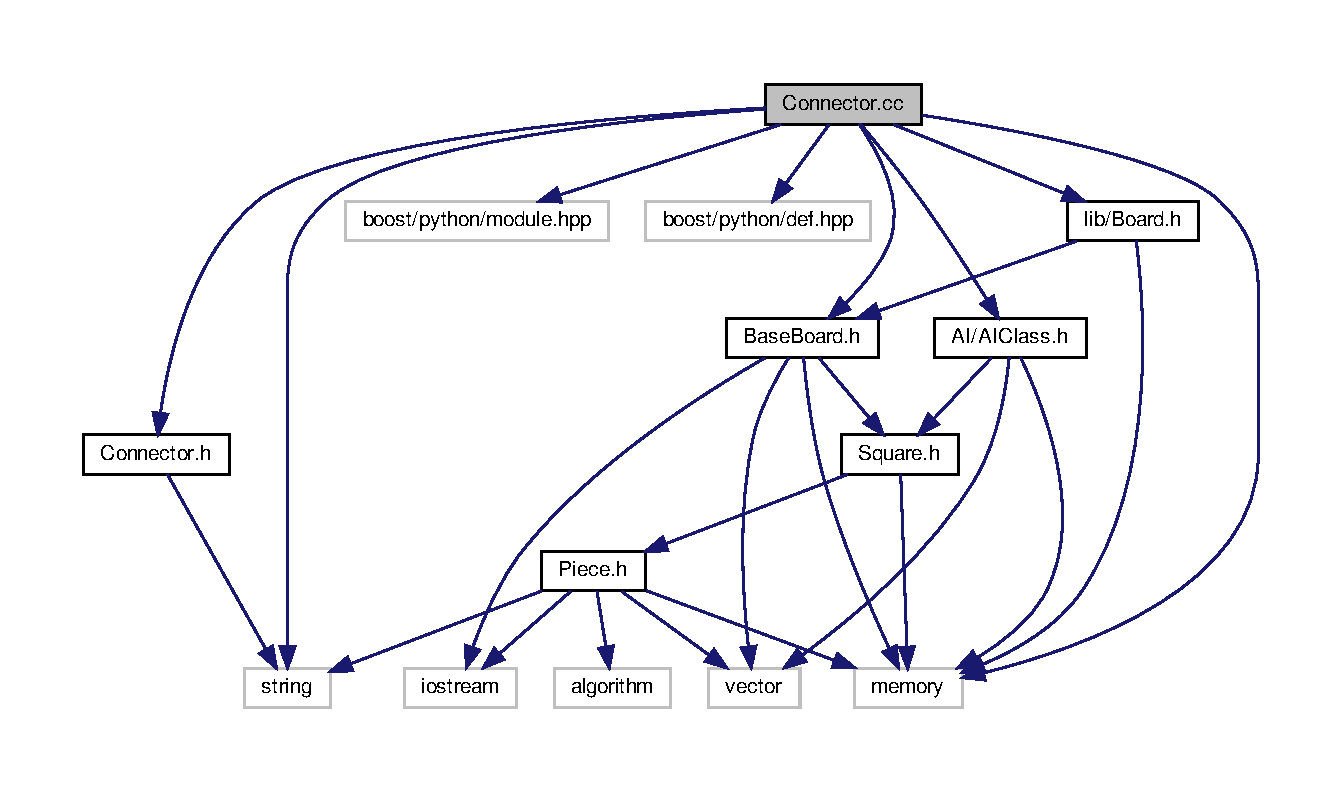
\includegraphics[width=350pt]{_connector_8cc__incl}
\end{center}
\end{figure}
\subsection*{Functions}
\begin{DoxyCompactItemize}
\item 
\hyperlink{_connector_8cc_a58e2523a7c74a69c6d400f7389116974}{B\+O\+O\+S\+T\+\_\+\+P\+Y\+T\+H\+O\+N\+\_\+\+M\+O\+D\+U\+LE} (libchesslib)
\end{DoxyCompactItemize}


\subsection{Function Documentation}
\mbox{\Hypertarget{_connector_8cc_a58e2523a7c74a69c6d400f7389116974}\label{_connector_8cc_a58e2523a7c74a69c6d400f7389116974}} 
\index{Connector.\+cc@{Connector.\+cc}!B\+O\+O\+S\+T\+\_\+\+P\+Y\+T\+H\+O\+N\+\_\+\+M\+O\+D\+U\+LE@{B\+O\+O\+S\+T\+\_\+\+P\+Y\+T\+H\+O\+N\+\_\+\+M\+O\+D\+U\+LE}}
\index{B\+O\+O\+S\+T\+\_\+\+P\+Y\+T\+H\+O\+N\+\_\+\+M\+O\+D\+U\+LE@{B\+O\+O\+S\+T\+\_\+\+P\+Y\+T\+H\+O\+N\+\_\+\+M\+O\+D\+U\+LE}!Connector.\+cc@{Connector.\+cc}}
\subsubsection{\texorpdfstring{B\+O\+O\+S\+T\+\_\+\+P\+Y\+T\+H\+O\+N\+\_\+\+M\+O\+D\+U\+L\+E()}{BOOST\_PYTHON\_MODULE()}}
{\footnotesize\ttfamily B\+O\+O\+S\+T\+\_\+\+P\+Y\+T\+H\+O\+N\+\_\+\+M\+O\+D\+U\+LE (\begin{DoxyParamCaption}\item[{libchesslib}]{ }\end{DoxyParamCaption})}


\hypertarget{_connector_8h}{}\section{Connector.\+h File Reference}
\label{_connector_8h}\index{Connector.\+h@{Connector.\+h}}
{\ttfamily \#include $<$string$>$}\newline
Include dependency graph for Connector.\+h\+:\nopagebreak
\begin{figure}[H]
\begin{center}
\leavevmode
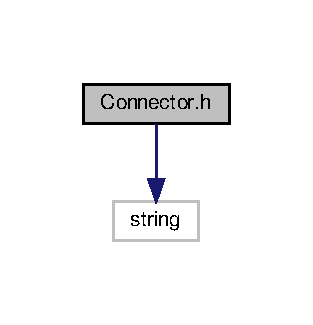
\includegraphics[width=150pt]{_connector_8h__incl}
\end{center}
\end{figure}
This graph shows which files directly or indirectly include this file\+:\nopagebreak
\begin{figure}[H]
\begin{center}
\leavevmode
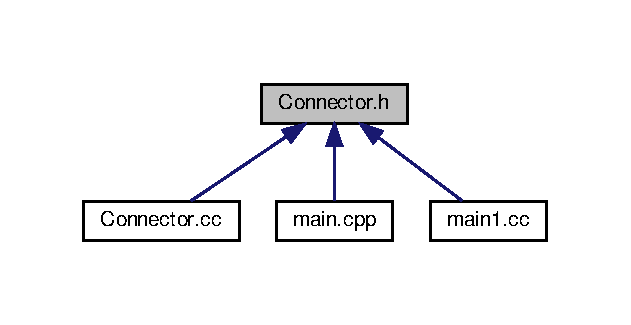
\includegraphics[width=303pt]{_connector_8h__dep__incl}
\end{center}
\end{figure}
\subsection*{Classes}
\begin{DoxyCompactItemize}
\item 
class \hyperlink{class_connector}{Connector}
\end{DoxyCompactItemize}

\hypertarget{_wrong_arg_exception_8cpp}{}\section{exceptions/\+Wrong\+Arg\+Exception.cpp File Reference}
\label{_wrong_arg_exception_8cpp}\index{exceptions/\+Wrong\+Arg\+Exception.\+cpp@{exceptions/\+Wrong\+Arg\+Exception.\+cpp}}
{\ttfamily \#include \char`\"{}Wrong\+Arg\+Exception.\+h\char`\"{}}\newline
Include dependency graph for Wrong\+Arg\+Exception.\+cpp\+:\nopagebreak
\begin{figure}[H]
\begin{center}
\leavevmode
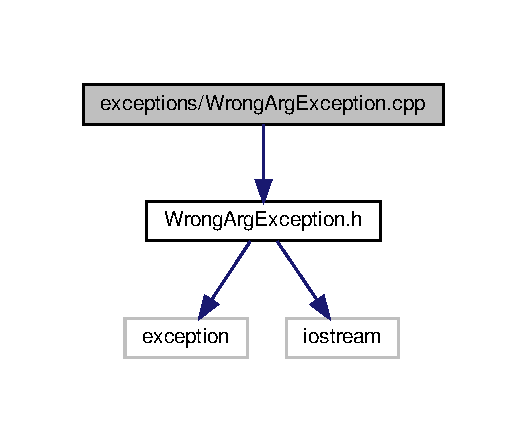
\includegraphics[width=253pt]{_wrong_arg_exception_8cpp__incl}
\end{center}
\end{figure}

\hypertarget{_wrong_arg_exception_8h}{}\section{exceptions/\+Wrong\+Arg\+Exception.h File Reference}
\label{_wrong_arg_exception_8h}\index{exceptions/\+Wrong\+Arg\+Exception.\+h@{exceptions/\+Wrong\+Arg\+Exception.\+h}}
{\ttfamily \#include $<$exception$>$}\newline
{\ttfamily \#include $<$iostream$>$}\newline
Include dependency graph for Wrong\+Arg\+Exception.\+h\+:\nopagebreak
\begin{figure}[H]
\begin{center}
\leavevmode
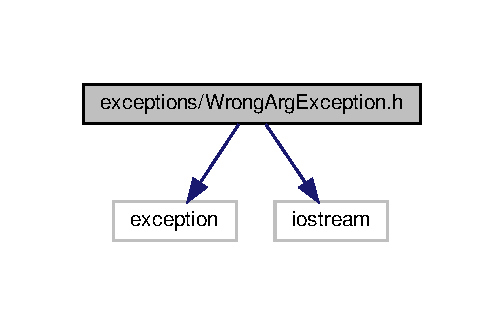
\includegraphics[width=242pt]{_wrong_arg_exception_8h__incl}
\end{center}
\end{figure}
This graph shows which files directly or indirectly include this file\+:\nopagebreak
\begin{figure}[H]
\begin{center}
\leavevmode
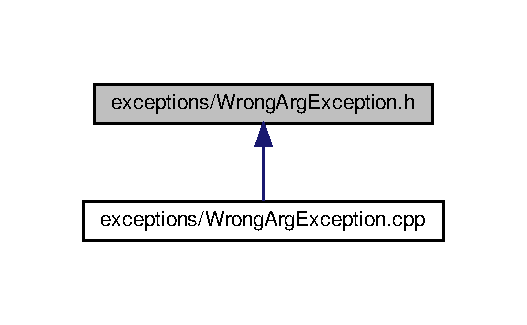
\includegraphics[width=253pt]{_wrong_arg_exception_8h__dep__incl}
\end{center}
\end{figure}
\subsection*{Classes}
\begin{DoxyCompactItemize}
\item 
class \hyperlink{class_wrong_arg_exception}{Wrong\+Arg\+Exception}
\end{DoxyCompactItemize}

\hypertarget{_king_8cc}{}\section{King.\+cc File Reference}
\label{_king_8cc}\index{King.\+cc@{King.\+cc}}
{\ttfamily \#include \char`\"{}lib/\+King.\+h\char`\"{}}\newline
{\ttfamily \#include $<$memory$>$}\newline
{\ttfamily \#include \char`\"{}A\+I/\+Position\+Value.\+h\char`\"{}}\newline
Include dependency graph for King.\+cc\+:\nopagebreak
\begin{figure}[H]
\begin{center}
\leavevmode
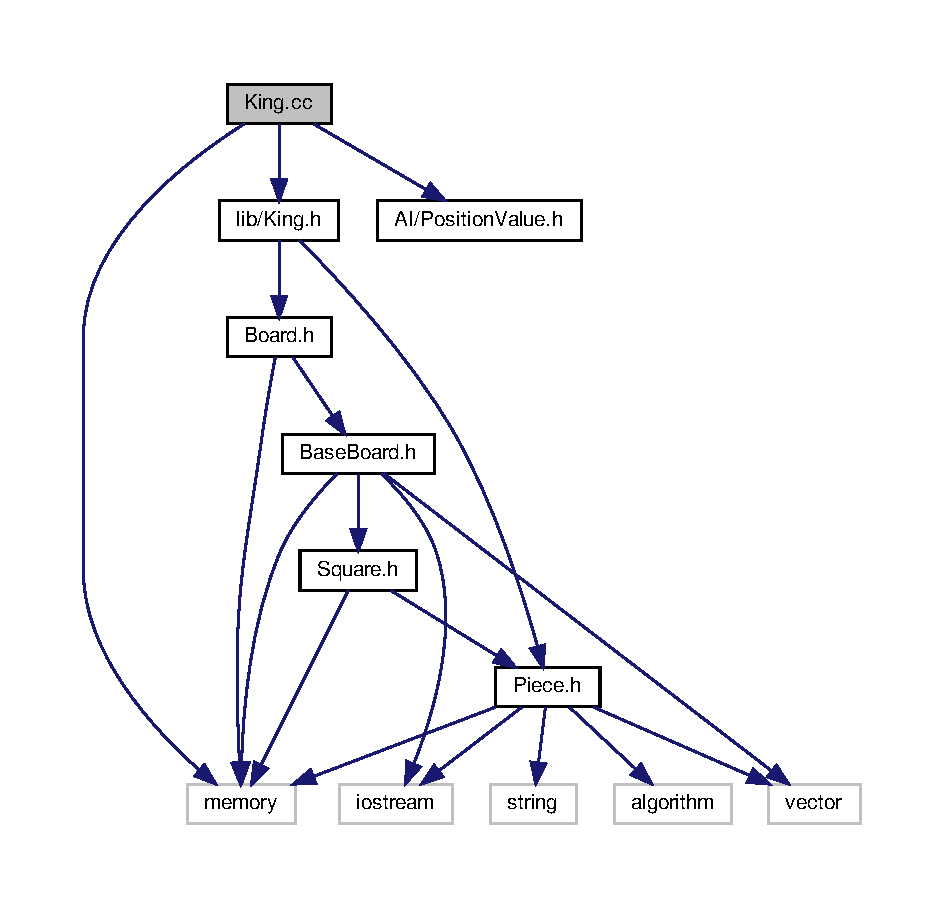
\includegraphics[width=350pt]{_king_8cc__incl}
\end{center}
\end{figure}

\hypertarget{_knight_8cc}{}\section{Knight.\+cc File Reference}
\label{_knight_8cc}\index{Knight.\+cc@{Knight.\+cc}}
{\ttfamily \#include \char`\"{}lib/\+Knight.\+h\char`\"{}}\newline
{\ttfamily \#include $<$memory$>$}\newline
{\ttfamily \#include \char`\"{}A\+I/\+Position\+Value.\+h\char`\"{}}\newline
Include dependency graph for Knight.\+cc\+:\nopagebreak
\begin{figure}[H]
\begin{center}
\leavevmode
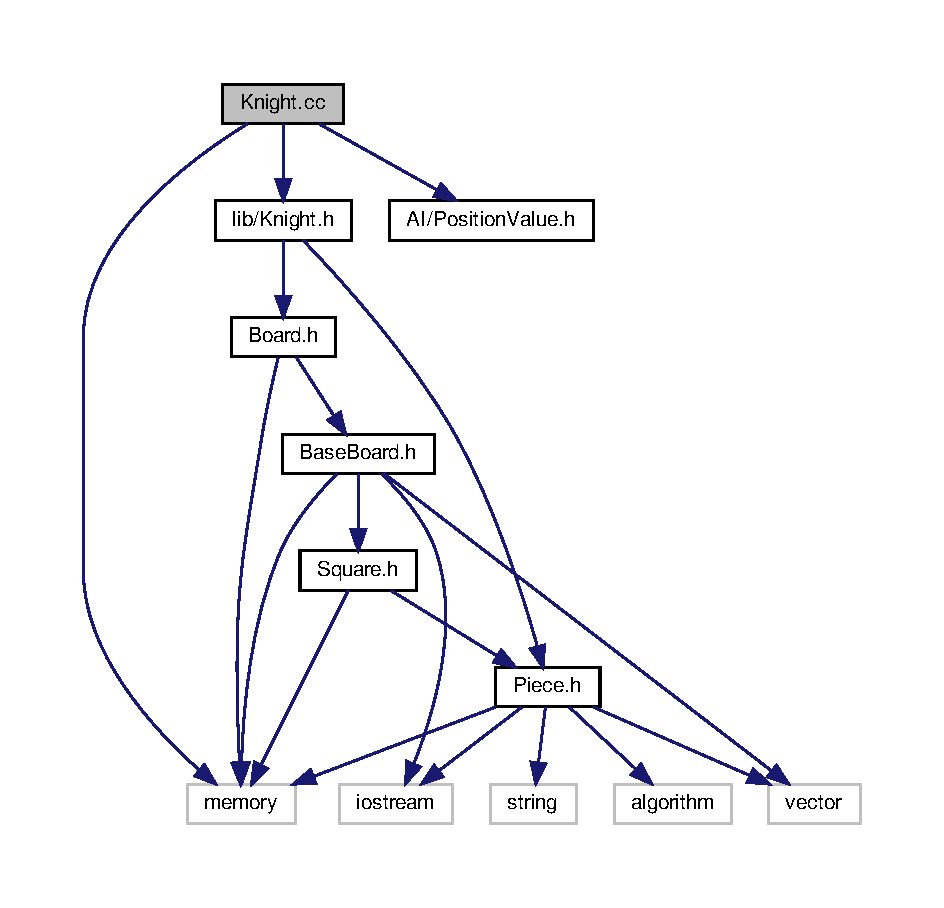
\includegraphics[width=350pt]{_knight_8cc__incl}
\end{center}
\end{figure}

\hypertarget{_base_board_8h}{}\section{lib/\+Base\+Board.h File Reference}
\label{_base_board_8h}\index{lib/\+Base\+Board.\+h@{lib/\+Base\+Board.\+h}}


Class holding informations about pieces, used to be an auxiliary class to generate temporary boards.  


{\ttfamily \#include \char`\"{}Square.\+h\char`\"{}}\newline
{\ttfamily \#include $<$vector$>$}\newline
{\ttfamily \#include $<$iostream$>$}\newline
{\ttfamily \#include $<$memory$>$}\newline
Include dependency graph for Base\+Board.\+h\+:\nopagebreak
\begin{figure}[H]
\begin{center}
\leavevmode
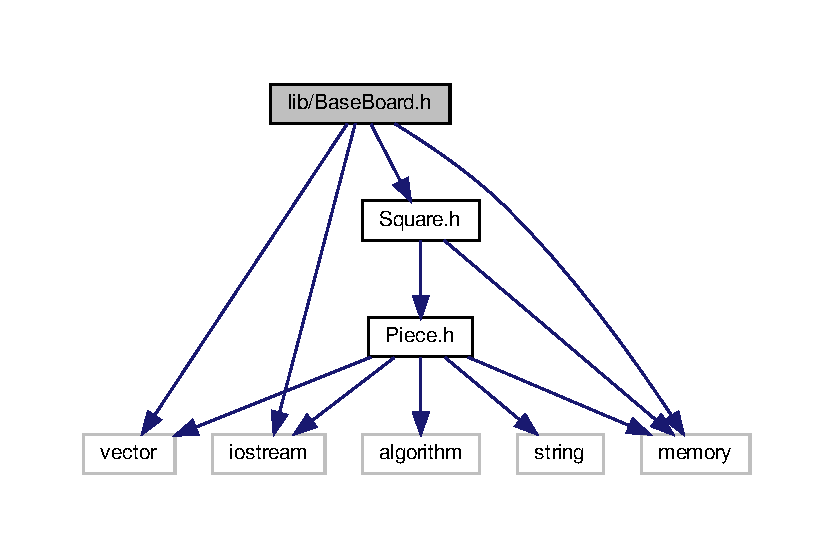
\includegraphics[width=350pt]{_base_board_8h__incl}
\end{center}
\end{figure}
This graph shows which files directly or indirectly include this file\+:\nopagebreak
\begin{figure}[H]
\begin{center}
\leavevmode
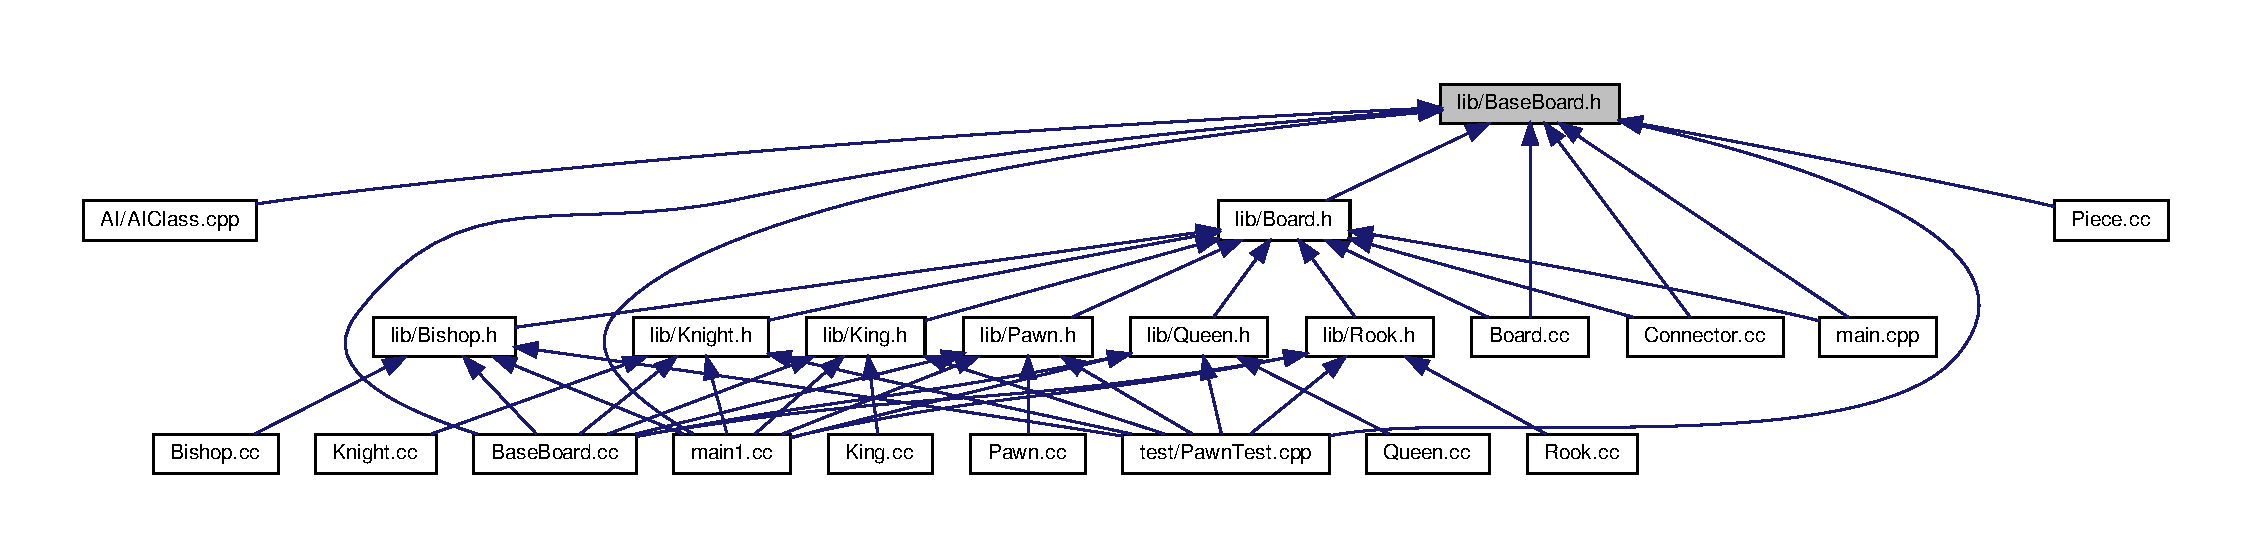
\includegraphics[width=350pt]{_base_board_8h__dep__incl}
\end{center}
\end{figure}
\subsection*{Classes}
\begin{DoxyCompactItemize}
\item 
class \hyperlink{class_base_board}{Base\+Board}
\end{DoxyCompactItemize}
\subsection*{Typedefs}
\begin{DoxyCompactItemize}
\item 
typedef std\+::vector$<$ std\+::vector$<$ std\+::shared\+\_\+ptr$<$ \hyperlink{class_square}{Square} $>$ $>$ $>$ \hyperlink{_base_board_8h_a6e73002e9c84a7986c39d7e80e83dc8d}{board\+\_\+type}
\end{DoxyCompactItemize}
\subsection*{Variables}
\begin{DoxyCompactItemize}
\item 
std\+::vector$<$ std\+::vector$<$ std\+::string $>$ $>$ const \hyperlink{_base_board_8h_a9965e03c4f48ae012bf1d93c397bf22c}{I\+N\+I\+T\+I\+A\+L\+\_\+\+B\+O\+A\+RD}
\begin{DoxyCompactList}\small\item\em vector used to initialize starting boards \end{DoxyCompactList}\end{DoxyCompactItemize}


\subsection{Detailed Description}
Class holding informations about pieces, used to be an auxiliary class to generate temporary boards. 

\begin{DoxyAuthor}{Author}
Marcin Michalski (\href{mailto:marmichalski97@gmail.com}{\tt marmichalski97@gmail.\+com}) 
\end{DoxyAuthor}
\begin{DoxyVersion}{Version}
0.\+1 
\end{DoxyVersion}
\begin{DoxyDate}{Date}
2020-\/01-\/15
\end{DoxyDate}
\begin{DoxyCopyright}{Copyright}
Copyright (c) 2020 
\end{DoxyCopyright}


\subsection{Typedef Documentation}
\mbox{\Hypertarget{_base_board_8h_a6e73002e9c84a7986c39d7e80e83dc8d}\label{_base_board_8h_a6e73002e9c84a7986c39d7e80e83dc8d}} 
\index{Base\+Board.\+h@{Base\+Board.\+h}!board\+\_\+type@{board\+\_\+type}}
\index{board\+\_\+type@{board\+\_\+type}!Base\+Board.\+h@{Base\+Board.\+h}}
\subsubsection{\texorpdfstring{board\+\_\+type}{board\_type}}
{\footnotesize\ttfamily typedef std\+::vector$<$std\+::vector $<$std\+::shared\+\_\+ptr$<$\hyperlink{class_square}{Square}$>$ $>$ $>$ \hyperlink{_a_i_class_8h_a6e73002e9c84a7986c39d7e80e83dc8d}{board\+\_\+type}}



\subsection{Variable Documentation}
\mbox{\Hypertarget{_base_board_8h_a9965e03c4f48ae012bf1d93c397bf22c}\label{_base_board_8h_a9965e03c4f48ae012bf1d93c397bf22c}} 
\index{Base\+Board.\+h@{Base\+Board.\+h}!I\+N\+I\+T\+I\+A\+L\+\_\+\+B\+O\+A\+RD@{I\+N\+I\+T\+I\+A\+L\+\_\+\+B\+O\+A\+RD}}
\index{I\+N\+I\+T\+I\+A\+L\+\_\+\+B\+O\+A\+RD@{I\+N\+I\+T\+I\+A\+L\+\_\+\+B\+O\+A\+RD}!Base\+Board.\+h@{Base\+Board.\+h}}
\subsubsection{\texorpdfstring{I\+N\+I\+T\+I\+A\+L\+\_\+\+B\+O\+A\+RD}{INITIAL\_BOARD}}
{\footnotesize\ttfamily std\+::vector$<$std\+::vector $<$std\+::string$>$ $>$ const I\+N\+I\+T\+I\+A\+L\+\_\+\+B\+O\+A\+RD}

{\bfseries Initial value\+:}
\begin{DoxyCode}
= \{
\{\textcolor{stringliteral}{"WR"},\textcolor{stringliteral}{"WP"},\textcolor{stringliteral}{"NN"},\textcolor{stringliteral}{"NN"},\textcolor{stringliteral}{"NN"},\textcolor{stringliteral}{"NN"},\textcolor{stringliteral}{"BP"},\textcolor{stringliteral}{"BR"}\},
\{\textcolor{stringliteral}{"WN"},\textcolor{stringliteral}{"WP"},\textcolor{stringliteral}{"NN"},\textcolor{stringliteral}{"NN"},\textcolor{stringliteral}{"NN"},\textcolor{stringliteral}{"NN"},\textcolor{stringliteral}{"BP"},\textcolor{stringliteral}{"BN"}\},
\{\textcolor{stringliteral}{"WB"},\textcolor{stringliteral}{"WP"},\textcolor{stringliteral}{"NN"},\textcolor{stringliteral}{"NN"},\textcolor{stringliteral}{"NN"},\textcolor{stringliteral}{"NN"},\textcolor{stringliteral}{"BP"},\textcolor{stringliteral}{"BB"}\},
\{\textcolor{stringliteral}{"WQ"},\textcolor{stringliteral}{"WP"},\textcolor{stringliteral}{"NN"},\textcolor{stringliteral}{"NN"},\textcolor{stringliteral}{"NN"},\textcolor{stringliteral}{"NN"},\textcolor{stringliteral}{"BP"},\textcolor{stringliteral}{"BQ"}\},
\{\textcolor{stringliteral}{"WK"},\textcolor{stringliteral}{"WP"},\textcolor{stringliteral}{"NN"},\textcolor{stringliteral}{"NN"},\textcolor{stringliteral}{"NN"},\textcolor{stringliteral}{"NN"},\textcolor{stringliteral}{"BP"},\textcolor{stringliteral}{"BK"}\},
\{\textcolor{stringliteral}{"WB"},\textcolor{stringliteral}{"WP"},\textcolor{stringliteral}{"NN"},\textcolor{stringliteral}{"NN"},\textcolor{stringliteral}{"NN"},\textcolor{stringliteral}{"NN"},\textcolor{stringliteral}{"BP"},\textcolor{stringliteral}{"BB"}\},
\{\textcolor{stringliteral}{"WN"},\textcolor{stringliteral}{"WP"},\textcolor{stringliteral}{"NN"},\textcolor{stringliteral}{"NN"},\textcolor{stringliteral}{"NN"},\textcolor{stringliteral}{"NN"},\textcolor{stringliteral}{"BP"},\textcolor{stringliteral}{"BN"}\},
\{\textcolor{stringliteral}{"WR"},\textcolor{stringliteral}{"WP"},\textcolor{stringliteral}{"NN"},\textcolor{stringliteral}{"NN"},\textcolor{stringliteral}{"NN"},\textcolor{stringliteral}{"NN"},\textcolor{stringliteral}{"BP"},\textcolor{stringliteral}{"BR"}\}

\}
\end{DoxyCode}


vector used to initialize starting boards 


\hypertarget{_bishop_8h}{}\section{lib/\+Bishop.h File Reference}
\label{_bishop_8h}\index{lib/\+Bishop.\+h@{lib/\+Bishop.\+h}}


Class for bishop.  


{\ttfamily \#include \char`\"{}Piece.\+h\char`\"{}}\newline
{\ttfamily \#include \char`\"{}Board.\+h\char`\"{}}\newline
Include dependency graph for Bishop.\+h\+:\nopagebreak
\begin{figure}[H]
\begin{center}
\leavevmode
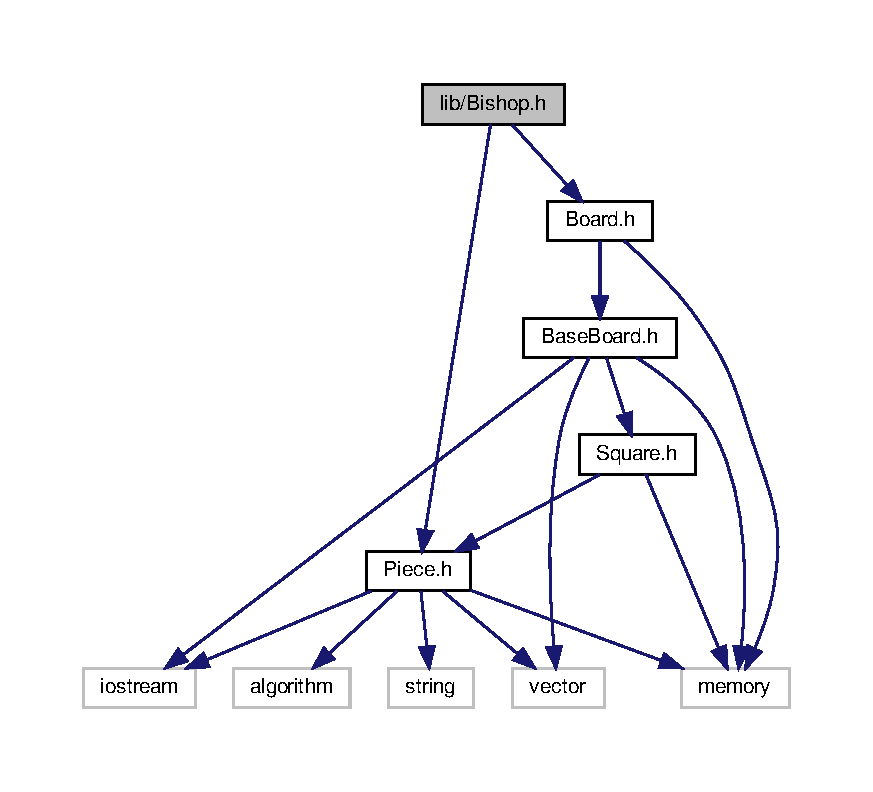
\includegraphics[width=350pt]{_bishop_8h__incl}
\end{center}
\end{figure}
This graph shows which files directly or indirectly include this file\+:\nopagebreak
\begin{figure}[H]
\begin{center}
\leavevmode
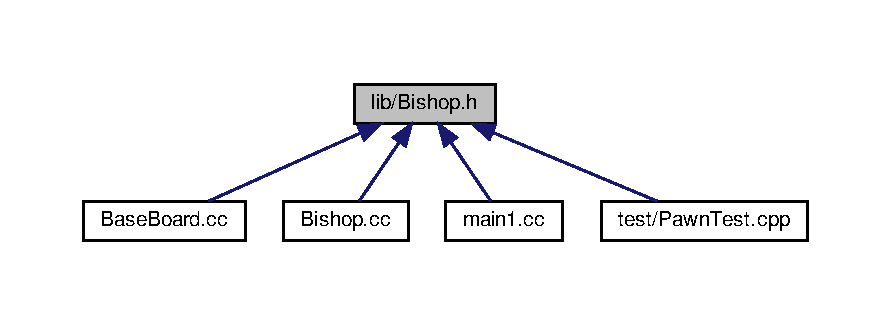
\includegraphics[width=350pt]{_bishop_8h__dep__incl}
\end{center}
\end{figure}
\subsection*{Classes}
\begin{DoxyCompactItemize}
\item 
class \hyperlink{class_bishop}{Bishop}
\end{DoxyCompactItemize}


\subsection{Detailed Description}
Class for bishop. 

\begin{DoxyAuthor}{Author}
Marcin Michalski (\href{mailto:marmichalski97@gmail.com}{\tt marmichalski97@gmail.\+com}) 
\end{DoxyAuthor}
\begin{DoxyVersion}{Version}
0.\+1 
\end{DoxyVersion}
\begin{DoxyDate}{Date}
2020-\/01-\/15
\end{DoxyDate}
\begin{DoxyCopyright}{Copyright}
Copyright (c) 2020 
\end{DoxyCopyright}

\hypertarget{_board_8h}{}\section{lib/\+Board.h File Reference}
\label{_board_8h}\index{lib/\+Board.\+h@{lib/\+Board.\+h}}
{\ttfamily \#include \char`\"{}Base\+Board.\+h\char`\"{}}\newline
{\ttfamily \#include $<$memory$>$}\newline
Include dependency graph for Board.\+h\+:\nopagebreak
\begin{figure}[H]
\begin{center}
\leavevmode
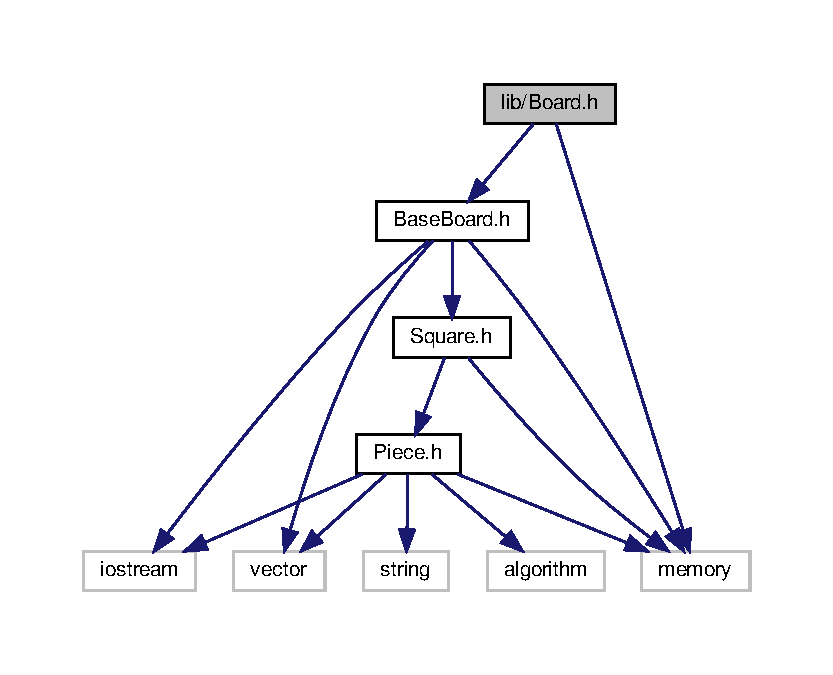
\includegraphics[width=350pt]{_board_8h__incl}
\end{center}
\end{figure}
This graph shows which files directly or indirectly include this file\+:\nopagebreak
\begin{figure}[H]
\begin{center}
\leavevmode
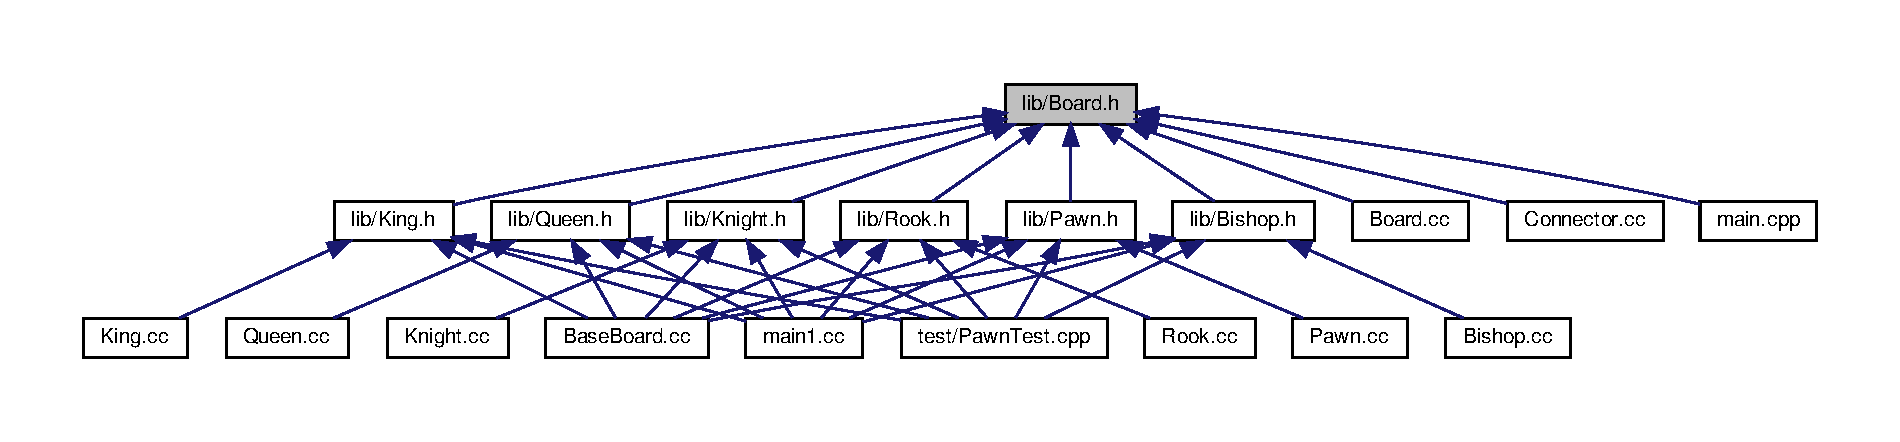
\includegraphics[width=350pt]{_board_8h__dep__incl}
\end{center}
\end{figure}
\subsection*{Classes}
\begin{DoxyCompactItemize}
\item 
class \hyperlink{class_board}{Board}
\end{DoxyCompactItemize}

\hypertarget{_king_8h}{}\section{lib/\+King.h File Reference}
\label{_king_8h}\index{lib/\+King.\+h@{lib/\+King.\+h}}
{\ttfamily \#include \char`\"{}Piece.\+h\char`\"{}}\newline
{\ttfamily \#include \char`\"{}Board.\+h\char`\"{}}\newline
Include dependency graph for King.\+h\+:\nopagebreak
\begin{figure}[H]
\begin{center}
\leavevmode
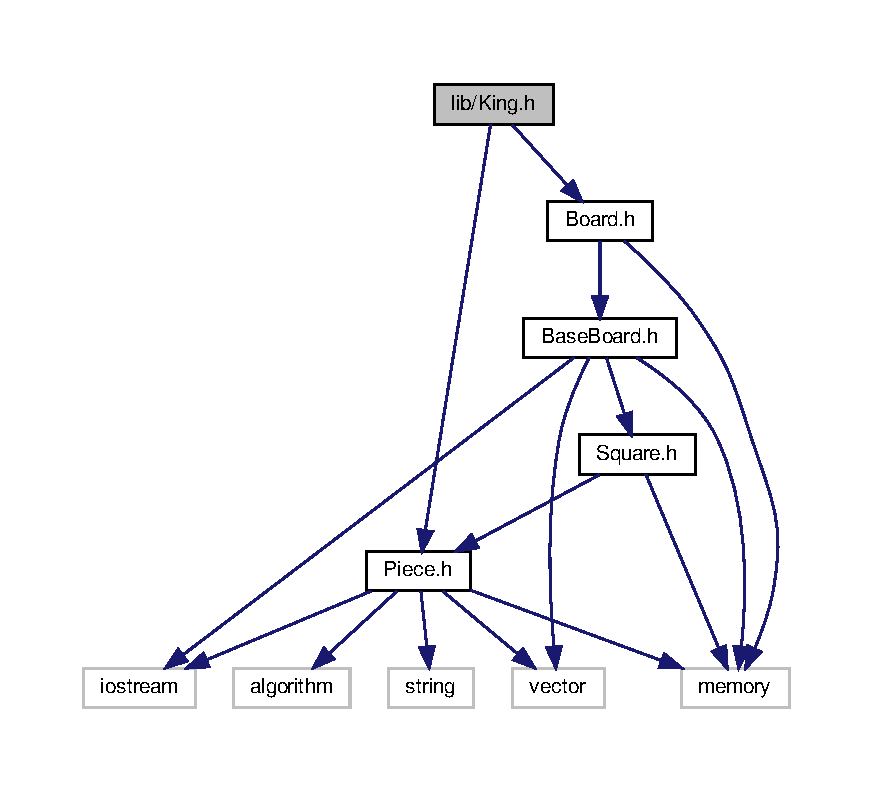
\includegraphics[width=350pt]{_king_8h__incl}
\end{center}
\end{figure}
This graph shows which files directly or indirectly include this file\+:\nopagebreak
\begin{figure}[H]
\begin{center}
\leavevmode
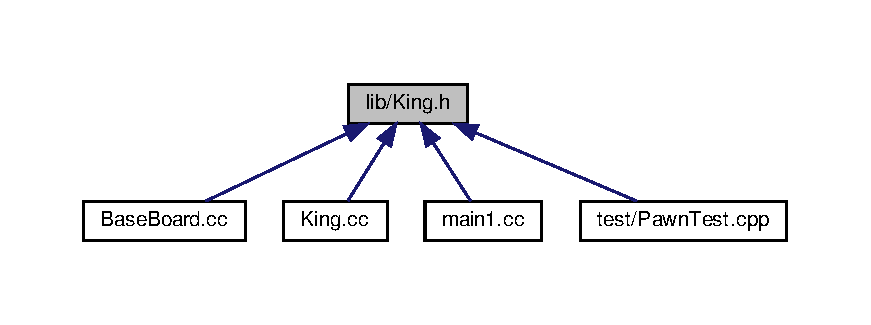
\includegraphics[width=350pt]{_king_8h__dep__incl}
\end{center}
\end{figure}
\subsection*{Classes}
\begin{DoxyCompactItemize}
\item 
class \hyperlink{class_king}{King}
\end{DoxyCompactItemize}

\hypertarget{_knight_8h}{}\section{lib/\+Knight.h File Reference}
\label{_knight_8h}\index{lib/\+Knight.\+h@{lib/\+Knight.\+h}}
{\ttfamily \#include \char`\"{}Piece.\+h\char`\"{}}\newline
{\ttfamily \#include \char`\"{}Board.\+h\char`\"{}}\newline
Include dependency graph for Knight.\+h\+:\nopagebreak
\begin{figure}[H]
\begin{center}
\leavevmode
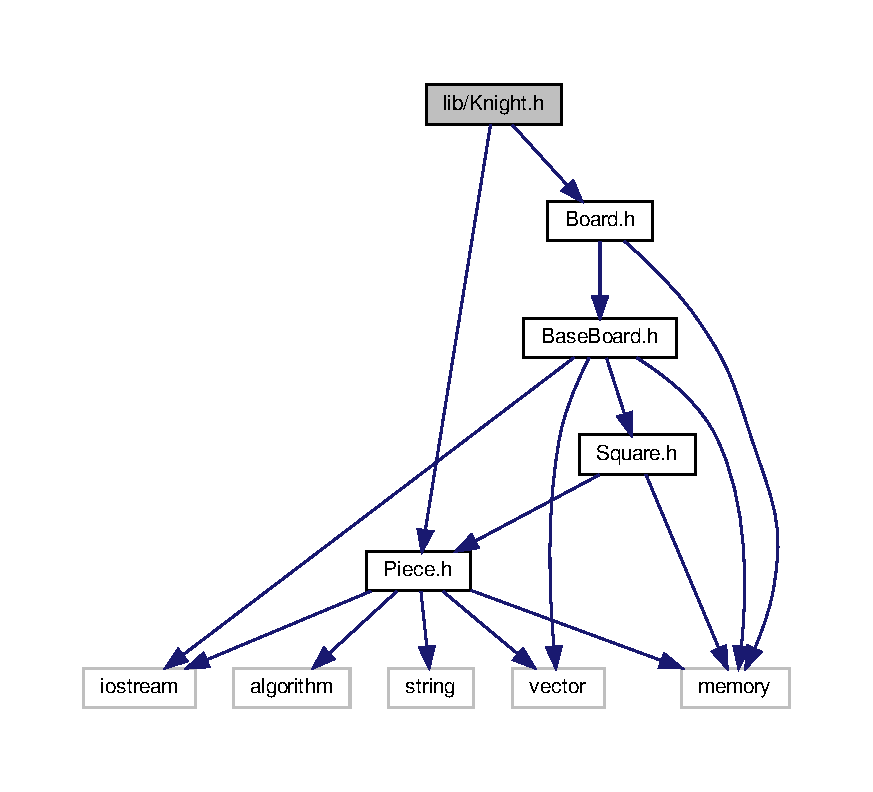
\includegraphics[width=350pt]{_knight_8h__incl}
\end{center}
\end{figure}
This graph shows which files directly or indirectly include this file\+:\nopagebreak
\begin{figure}[H]
\begin{center}
\leavevmode
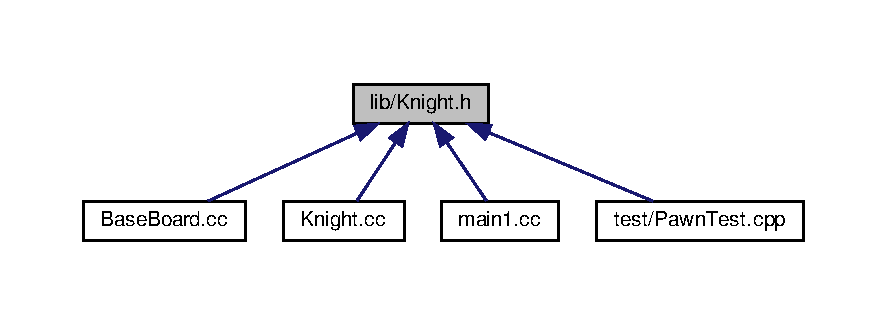
\includegraphics[width=350pt]{_knight_8h__dep__incl}
\end{center}
\end{figure}
\subsection*{Classes}
\begin{DoxyCompactItemize}
\item 
class \hyperlink{class_knight}{Knight}
\end{DoxyCompactItemize}


\subsection{Detailed Description}
\begin{DoxyAuthor}{Author}
Marcin Michalski (\href{mailto:marmichalski97@gmail.com}{\tt marmichalski97@gmail.\+com}) 
\end{DoxyAuthor}
\begin{DoxyVersion}{Version}
0.\+1 
\end{DoxyVersion}
\begin{DoxyDate}{Date}
2020-\/01-\/15
\end{DoxyDate}
\begin{DoxyCopyright}{Copyright}
Copyright (c) 2020 
\end{DoxyCopyright}

\hypertarget{_pawn_8h}{}\section{lib/\+Pawn.h File Reference}
\label{_pawn_8h}\index{lib/\+Pawn.\+h@{lib/\+Pawn.\+h}}
{\ttfamily \#include \char`\"{}Piece.\+h\char`\"{}}\newline
{\ttfamily \#include \char`\"{}Board.\+h\char`\"{}}\newline
{\ttfamily \#include $<$algorithm$>$}\newline
{\ttfamily \#include $<$iostream$>$}\newline
Include dependency graph for Pawn.\+h\+:\nopagebreak
\begin{figure}[H]
\begin{center}
\leavevmode
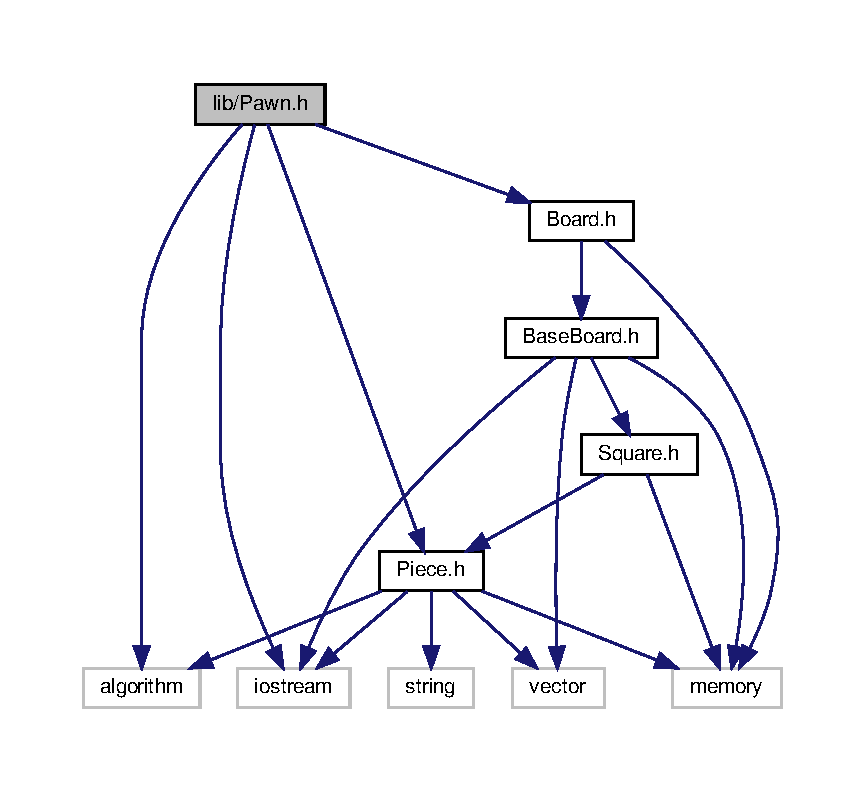
\includegraphics[width=350pt]{_pawn_8h__incl}
\end{center}
\end{figure}
This graph shows which files directly or indirectly include this file\+:\nopagebreak
\begin{figure}[H]
\begin{center}
\leavevmode
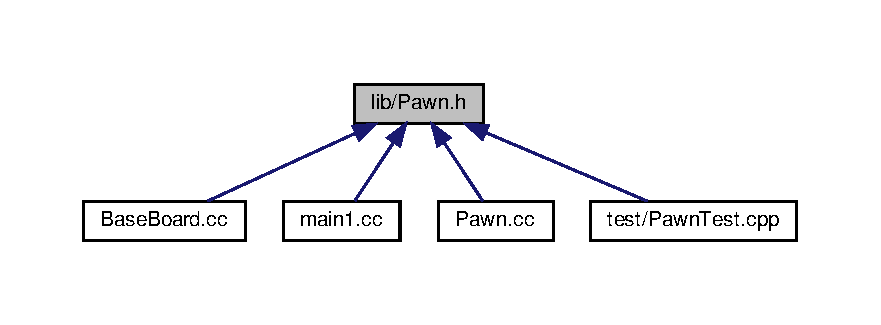
\includegraphics[width=350pt]{_pawn_8h__dep__incl}
\end{center}
\end{figure}
\subsection*{Classes}
\begin{DoxyCompactItemize}
\item 
class \hyperlink{class_pawn}{Pawn}
\end{DoxyCompactItemize}


\subsection{Detailed Description}
\begin{DoxyAuthor}{Author}
Marcin Michalski (\href{mailto:marmichalski97@gmail.com}{\tt marmichalski97@gmail.\+com}) 
\end{DoxyAuthor}
\begin{DoxyVersion}{Version}
0.\+1 
\end{DoxyVersion}
\begin{DoxyDate}{Date}
2020-\/01-\/15
\end{DoxyDate}
\begin{DoxyCopyright}{Copyright}
Copyright (c) 2020 
\end{DoxyCopyright}

\hypertarget{_piece_8h}{}\section{lib/\+Piece.h File Reference}
\label{_piece_8h}\index{lib/\+Piece.\+h@{lib/\+Piece.\+h}}
{\ttfamily \#include $<$string$>$}\newline
{\ttfamily \#include $<$vector$>$}\newline
{\ttfamily \#include $<$algorithm$>$}\newline
{\ttfamily \#include $<$iostream$>$}\newline
{\ttfamily \#include $<$memory$>$}\newline
Include dependency graph for Piece.\+h\+:\nopagebreak
\begin{figure}[H]
\begin{center}
\leavevmode
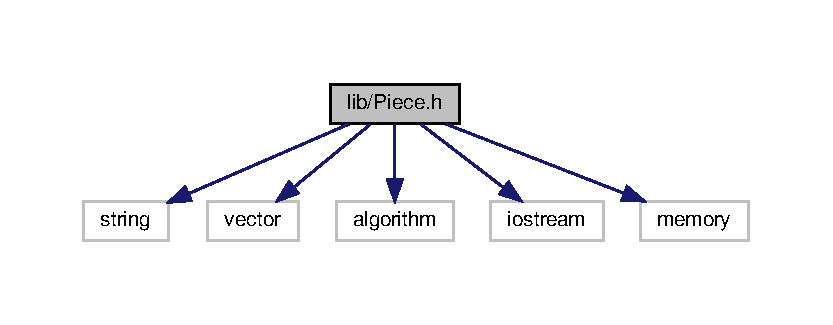
\includegraphics[width=350pt]{_piece_8h__incl}
\end{center}
\end{figure}
This graph shows which files directly or indirectly include this file\+:
\nopagebreak
\begin{figure}[H]
\begin{center}
\leavevmode
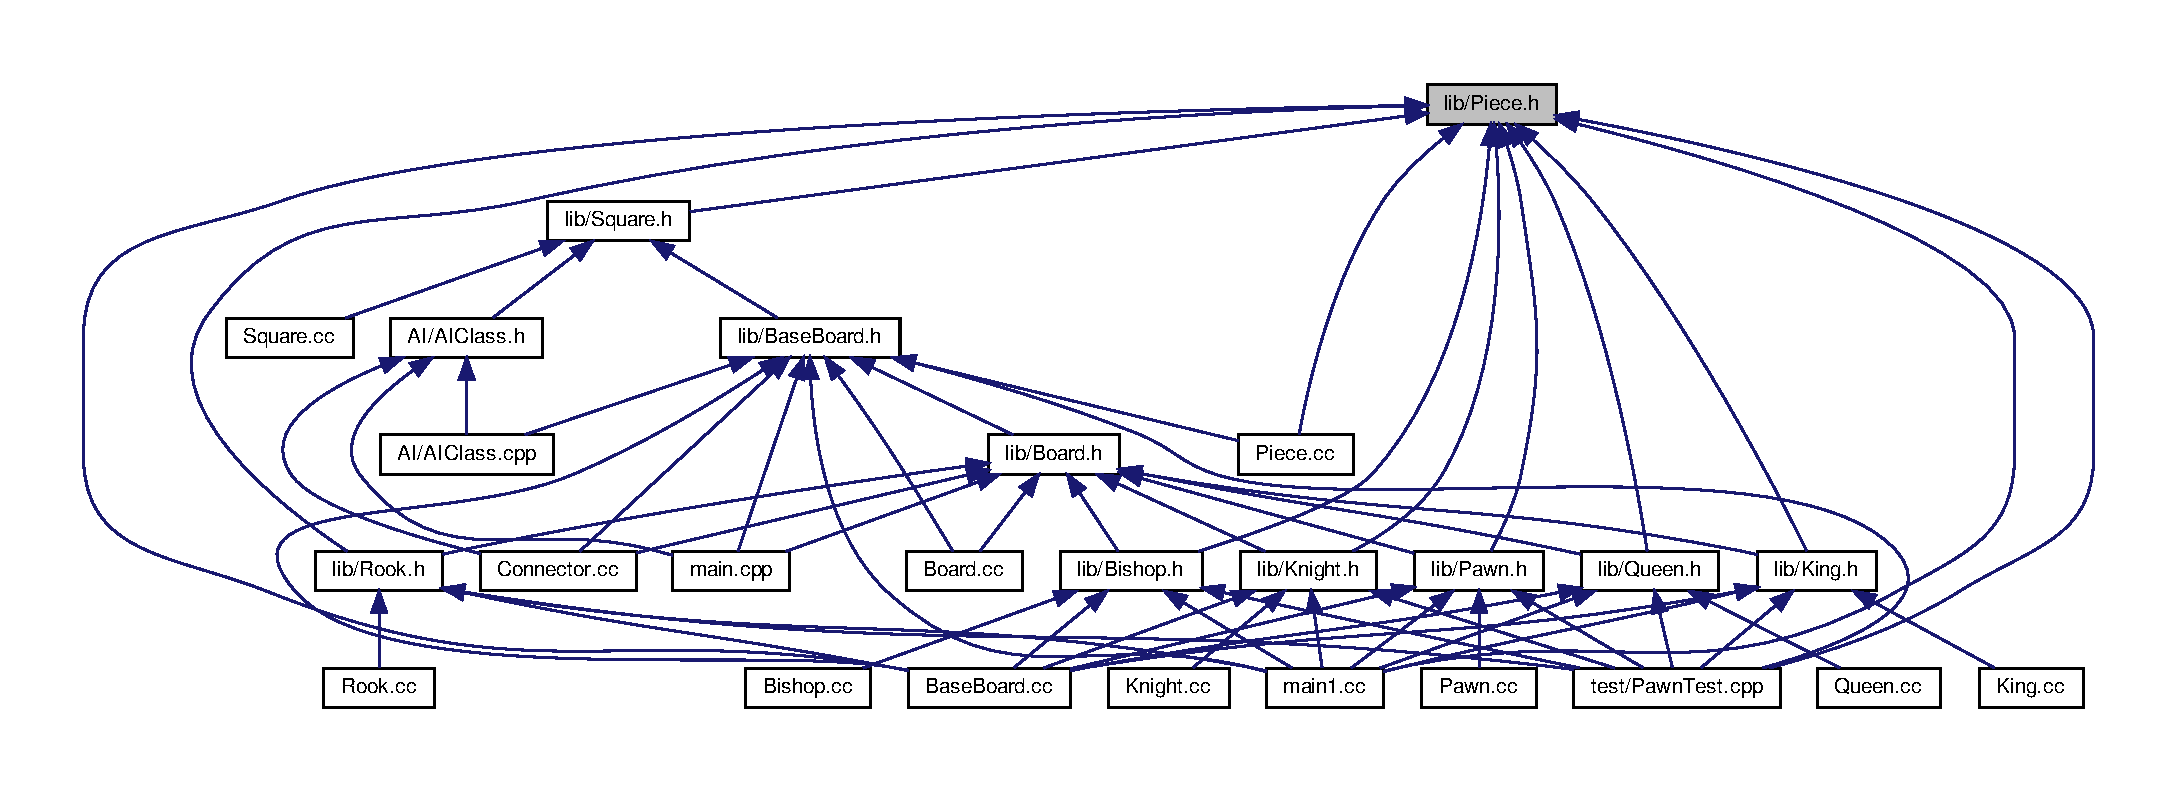
\includegraphics[width=350pt]{_piece_8h__dep__incl}
\end{center}
\end{figure}
\subsection*{Classes}
\begin{DoxyCompactItemize}
\item 
struct \hyperlink{struct_position}{Position}
\item 
class \hyperlink{class_piece}{Piece}
\end{DoxyCompactItemize}
\subsection*{Enumerations}
\begin{DoxyCompactItemize}
\item 
enum \hyperlink{_piece_8h_ad7595c48bb74c0dd2a7648712a2d4985}{Piece\+Color} \{ \hyperlink{_piece_8h_ad7595c48bb74c0dd2a7648712a2d4985af77fb67151d0c18d397069ad8c271ba3}{B\+L\+A\+CK} = -\/1, 
\hyperlink{_piece_8h_ad7595c48bb74c0dd2a7648712a2d4985a283fc479650da98250635b9c3c0e7e50}{W\+H\+I\+TE} = 1
 \}
\end{DoxyCompactItemize}
\subsection*{Variables}
\begin{DoxyCompactItemize}
\item 
const int \hyperlink{_piece_8h_a6584e1f78afd21bb3f138257c67dad87}{R\+O\+W\+\_\+\+M\+IN} = 0
\item 
const int \hyperlink{_piece_8h_ab601172ac2986c712422125c92d29efc}{C\+O\+L\+U\+M\+N\+\_\+\+M\+IN} = 0
\item 
const int \hyperlink{_piece_8h_a20c9fd20c215f832762c078722b2e3dd}{R\+O\+W\+\_\+\+M\+AX} = 8
\item 
const int \hyperlink{_piece_8h_ab6975f91acab5e76768eb60f3ddaa242}{C\+O\+L\+U\+M\+N\+\_\+\+M\+AX} = 8
\end{DoxyCompactItemize}


\subsection{Enumeration Type Documentation}
\mbox{\Hypertarget{_piece_8h_ad7595c48bb74c0dd2a7648712a2d4985}\label{_piece_8h_ad7595c48bb74c0dd2a7648712a2d4985}} 
\index{Piece.\+h@{Piece.\+h}!Piece\+Color@{Piece\+Color}}
\index{Piece\+Color@{Piece\+Color}!Piece.\+h@{Piece.\+h}}
\subsubsection{\texorpdfstring{Piece\+Color}{PieceColor}}
{\footnotesize\ttfamily enum \hyperlink{_piece_8h_ad7595c48bb74c0dd2a7648712a2d4985}{Piece\+Color}}

\begin{DoxyEnumFields}{Enumerator}
\raisebox{\heightof{T}}[0pt][0pt]{\index{B\+L\+A\+CK@{B\+L\+A\+CK}!Piece.\+h@{Piece.\+h}}\index{Piece.\+h@{Piece.\+h}!B\+L\+A\+CK@{B\+L\+A\+CK}}}\mbox{\Hypertarget{_piece_8h_ad7595c48bb74c0dd2a7648712a2d4985af77fb67151d0c18d397069ad8c271ba3}\label{_piece_8h_ad7595c48bb74c0dd2a7648712a2d4985af77fb67151d0c18d397069ad8c271ba3}} 
B\+L\+A\+CK&\\
\hline

\raisebox{\heightof{T}}[0pt][0pt]{\index{W\+H\+I\+TE@{W\+H\+I\+TE}!Piece.\+h@{Piece.\+h}}\index{Piece.\+h@{Piece.\+h}!W\+H\+I\+TE@{W\+H\+I\+TE}}}\mbox{\Hypertarget{_piece_8h_ad7595c48bb74c0dd2a7648712a2d4985a283fc479650da98250635b9c3c0e7e50}\label{_piece_8h_ad7595c48bb74c0dd2a7648712a2d4985a283fc479650da98250635b9c3c0e7e50}} 
W\+H\+I\+TE&\\
\hline

\end{DoxyEnumFields}


\subsection{Variable Documentation}
\mbox{\Hypertarget{_piece_8h_ab6975f91acab5e76768eb60f3ddaa242}\label{_piece_8h_ab6975f91acab5e76768eb60f3ddaa242}} 
\index{Piece.\+h@{Piece.\+h}!C\+O\+L\+U\+M\+N\+\_\+\+M\+AX@{C\+O\+L\+U\+M\+N\+\_\+\+M\+AX}}
\index{C\+O\+L\+U\+M\+N\+\_\+\+M\+AX@{C\+O\+L\+U\+M\+N\+\_\+\+M\+AX}!Piece.\+h@{Piece.\+h}}
\subsubsection{\texorpdfstring{C\+O\+L\+U\+M\+N\+\_\+\+M\+AX}{COLUMN\_MAX}}
{\footnotesize\ttfamily const int C\+O\+L\+U\+M\+N\+\_\+\+M\+AX = 8}

\mbox{\Hypertarget{_piece_8h_ab601172ac2986c712422125c92d29efc}\label{_piece_8h_ab601172ac2986c712422125c92d29efc}} 
\index{Piece.\+h@{Piece.\+h}!C\+O\+L\+U\+M\+N\+\_\+\+M\+IN@{C\+O\+L\+U\+M\+N\+\_\+\+M\+IN}}
\index{C\+O\+L\+U\+M\+N\+\_\+\+M\+IN@{C\+O\+L\+U\+M\+N\+\_\+\+M\+IN}!Piece.\+h@{Piece.\+h}}
\subsubsection{\texorpdfstring{C\+O\+L\+U\+M\+N\+\_\+\+M\+IN}{COLUMN\_MIN}}
{\footnotesize\ttfamily const int C\+O\+L\+U\+M\+N\+\_\+\+M\+IN = 0}

\mbox{\Hypertarget{_piece_8h_a20c9fd20c215f832762c078722b2e3dd}\label{_piece_8h_a20c9fd20c215f832762c078722b2e3dd}} 
\index{Piece.\+h@{Piece.\+h}!R\+O\+W\+\_\+\+M\+AX@{R\+O\+W\+\_\+\+M\+AX}}
\index{R\+O\+W\+\_\+\+M\+AX@{R\+O\+W\+\_\+\+M\+AX}!Piece.\+h@{Piece.\+h}}
\subsubsection{\texorpdfstring{R\+O\+W\+\_\+\+M\+AX}{ROW\_MAX}}
{\footnotesize\ttfamily const int R\+O\+W\+\_\+\+M\+AX = 8}

\mbox{\Hypertarget{_piece_8h_a6584e1f78afd21bb3f138257c67dad87}\label{_piece_8h_a6584e1f78afd21bb3f138257c67dad87}} 
\index{Piece.\+h@{Piece.\+h}!R\+O\+W\+\_\+\+M\+IN@{R\+O\+W\+\_\+\+M\+IN}}
\index{R\+O\+W\+\_\+\+M\+IN@{R\+O\+W\+\_\+\+M\+IN}!Piece.\+h@{Piece.\+h}}
\subsubsection{\texorpdfstring{R\+O\+W\+\_\+\+M\+IN}{ROW\_MIN}}
{\footnotesize\ttfamily const int R\+O\+W\+\_\+\+M\+IN = 0}


\hypertarget{_queen_8h}{}\section{lib/\+Queen.h File Reference}
\label{_queen_8h}\index{lib/\+Queen.\+h@{lib/\+Queen.\+h}}
{\ttfamily \#include \char`\"{}Piece.\+h\char`\"{}}\newline
{\ttfamily \#include \char`\"{}Board.\+h\char`\"{}}\newline
Include dependency graph for Queen.\+h\+:\nopagebreak
\begin{figure}[H]
\begin{center}
\leavevmode
\includegraphics[width=350pt]{_queen_8h__incl}
\end{center}
\end{figure}
This graph shows which files directly or indirectly include this file\+:\nopagebreak
\begin{figure}[H]
\begin{center}
\leavevmode
\includegraphics[width=350pt]{_queen_8h__dep__incl}
\end{center}
\end{figure}
\subsection*{Classes}
\begin{DoxyCompactItemize}
\item 
class \hyperlink{class_queen}{Queen}
\end{DoxyCompactItemize}


\subsection{Detailed Description}
\begin{DoxyAuthor}{Author}
Marcin Michalski (\href{mailto:marmichalski97@gmail.com}{\tt marmichalski97@gmail.\+com}) 
\end{DoxyAuthor}
\begin{DoxyVersion}{Version}
0.\+1 
\end{DoxyVersion}
\begin{DoxyDate}{Date}
2020-\/01-\/15
\end{DoxyDate}
\begin{DoxyCopyright}{Copyright}
Copyright (c) 2020 
\end{DoxyCopyright}

\hypertarget{_rook_8h}{}\section{lib/\+Rook.h File Reference}
\label{_rook_8h}\index{lib/\+Rook.\+h@{lib/\+Rook.\+h}}
{\ttfamily \#include \char`\"{}Piece.\+h\char`\"{}}\newline
{\ttfamily \#include \char`\"{}Board.\+h\char`\"{}}\newline
Include dependency graph for Rook.\+h\+:\nopagebreak
\begin{figure}[H]
\begin{center}
\leavevmode
\includegraphics[width=350pt]{_rook_8h__incl}
\end{center}
\end{figure}
This graph shows which files directly or indirectly include this file\+:\nopagebreak
\begin{figure}[H]
\begin{center}
\leavevmode
\includegraphics[width=350pt]{_rook_8h__dep__incl}
\end{center}
\end{figure}
\subsection*{Classes}
\begin{DoxyCompactItemize}
\item 
class \hyperlink{class_rook}{Rook}
\end{DoxyCompactItemize}


\subsection{Detailed Description}
\begin{DoxyAuthor}{Author}
Marcin Michalski (\href{mailto:marmichalski97@gmail.com}{\tt marmichalski97@gmail.\+com}) 
\end{DoxyAuthor}
\begin{DoxyVersion}{Version}
0.\+1 
\end{DoxyVersion}
\begin{DoxyDate}{Date}
2020-\/01-\/15
\end{DoxyDate}
\begin{DoxyCopyright}{Copyright}
Copyright (c) 2020 
\end{DoxyCopyright}

\hypertarget{_square_8h}{}\section{lib/\+Square.h File Reference}
\label{_square_8h}\index{lib/\+Square.\+h@{lib/\+Square.\+h}}
{\ttfamily \#include \char`\"{}Piece.\+h\char`\"{}}\newline
{\ttfamily \#include $<$memory$>$}\newline
Include dependency graph for Square.\+h\+:\nopagebreak
\begin{figure}[H]
\begin{center}
\leavevmode
\includegraphics[width=350pt]{_square_8h__incl}
\end{center}
\end{figure}
This graph shows which files directly or indirectly include this file\+:
\nopagebreak
\begin{figure}[H]
\begin{center}
\leavevmode
\includegraphics[width=350pt]{_square_8h__dep__incl}
\end{center}
\end{figure}
\subsection*{Classes}
\begin{DoxyCompactItemize}
\item 
class \hyperlink{class_square}{Square}
\end{DoxyCompactItemize}

\hypertarget{main_8cpp}{}\section{main.\+cpp File Reference}
\label{main_8cpp}\index{main.\+cpp@{main.\+cpp}}
{\ttfamily \#include \char`\"{}lib/\+Board.\+h\char`\"{}}\newline
{\ttfamily \#include $<$iostream$>$}\newline
{\ttfamily \#include \char`\"{}Connector.\+h\char`\"{}}\newline
{\ttfamily \#include \char`\"{}A\+I/\+A\+I\+Class.\+h\char`\"{}}\newline
{\ttfamily \#include \char`\"{}lib/\+Base\+Board.\+h\char`\"{}}\newline
Include dependency graph for main.\+cpp\+:\nopagebreak
\begin{figure}[H]
\begin{center}
\leavevmode
\includegraphics[width=350pt]{main_8cpp__incl}
\end{center}
\end{figure}
\subsection*{Functions}
\begin{DoxyCompactItemize}
\item 
int \hyperlink{main_8cpp_a840291bc02cba5474a4cb46a9b9566fe}{main} (void)
\end{DoxyCompactItemize}


\subsection{Function Documentation}
\mbox{\Hypertarget{main_8cpp_a840291bc02cba5474a4cb46a9b9566fe}\label{main_8cpp_a840291bc02cba5474a4cb46a9b9566fe}} 
\index{main.\+cpp@{main.\+cpp}!main@{main}}
\index{main@{main}!main.\+cpp@{main.\+cpp}}
\subsubsection{\texorpdfstring{main()}{main()}}
{\footnotesize\ttfamily int main (\begin{DoxyParamCaption}\item[{void}]{ }\end{DoxyParamCaption})}


\hypertarget{main1_8cc}{}\section{main1.\+cc File Reference}
\label{main1_8cc}\index{main1.\+cc@{main1.\+cc}}
{\ttfamily \#include \char`\"{}lib/\+Base\+Board.\+h\char`\"{}}\newline
{\ttfamily \#include $<$iostream$>$}\newline
{\ttfamily \#include \char`\"{}lib/\+Piece.\+h\char`\"{}}\newline
{\ttfamily \#include \char`\"{}lib/\+Bishop.\+h\char`\"{}}\newline
{\ttfamily \#include \char`\"{}lib/\+Rook.\+h\char`\"{}}\newline
{\ttfamily \#include \char`\"{}lib/\+Knight.\+h\char`\"{}}\newline
{\ttfamily \#include \char`\"{}lib/\+King.\+h\char`\"{}}\newline
{\ttfamily \#include \char`\"{}lib/\+Queen.\+h\char`\"{}}\newline
{\ttfamily \#include \char`\"{}lib/\+Pawn.\+h\char`\"{}}\newline
{\ttfamily \#include \char`\"{}Connector.\+h\char`\"{}}\newline
Include dependency graph for main1.\+cc\+:
\nopagebreak
\begin{figure}[H]
\begin{center}
\leavevmode
\includegraphics[width=350pt]{main1_8cc__incl}
\end{center}
\end{figure}
\subsection*{Functions}
\begin{DoxyCompactItemize}
\item 
int \hyperlink{main1_8cc_a840291bc02cba5474a4cb46a9b9566fe}{main} (void)
\end{DoxyCompactItemize}


\subsection{Function Documentation}
\mbox{\Hypertarget{main1_8cc_a840291bc02cba5474a4cb46a9b9566fe}\label{main1_8cc_a840291bc02cba5474a4cb46a9b9566fe}} 
\index{main1.\+cc@{main1.\+cc}!main@{main}}
\index{main@{main}!main1.\+cc@{main1.\+cc}}
\subsubsection{\texorpdfstring{main()}{main()}}
{\footnotesize\ttfamily int main (\begin{DoxyParamCaption}\item[{void}]{ }\end{DoxyParamCaption})}


\hypertarget{_pawn_8cc}{}\section{Pawn.\+cc File Reference}
\label{_pawn_8cc}\index{Pawn.\+cc@{Pawn.\+cc}}
{\ttfamily \#include \char`\"{}lib/\+Pawn.\+h\char`\"{}}\newline
{\ttfamily \#include $<$memory$>$}\newline
{\ttfamily \#include \char`\"{}A\+I/\+Position\+Value.\+h\char`\"{}}\newline
Include dependency graph for Pawn.\+cc\+:\nopagebreak
\begin{figure}[H]
\begin{center}
\leavevmode
\includegraphics[width=350pt]{_pawn_8cc__incl}
\end{center}
\end{figure}

\hypertarget{_piece_8cc}{}\section{Piece.\+cc File Reference}
\label{_piece_8cc}\index{Piece.\+cc@{Piece.\+cc}}
{\ttfamily \#include \char`\"{}lib/\+Piece.\+h\char`\"{}}\newline
{\ttfamily \#include \char`\"{}lib/\+Base\+Board.\+h\char`\"{}}\newline
Include dependency graph for Piece.\+cc\+:\nopagebreak
\begin{figure}[H]
\begin{center}
\leavevmode
\includegraphics[width=350pt]{_piece_8cc__incl}
\end{center}
\end{figure}

\hypertarget{_queen_8cc}{}\section{Queen.\+cc File Reference}
\label{_queen_8cc}\index{Queen.\+cc@{Queen.\+cc}}
{\ttfamily \#include \char`\"{}lib/\+Queen.\+h\char`\"{}}\newline
{\ttfamily \#include $<$memory$>$}\newline
{\ttfamily \#include \char`\"{}A\+I/\+Position\+Value.\+h\char`\"{}}\newline
Include dependency graph for Queen.\+cc\+:\nopagebreak
\begin{figure}[H]
\begin{center}
\leavevmode
\includegraphics[width=350pt]{_queen_8cc__incl}
\end{center}
\end{figure}

\hypertarget{_rook_8cc}{}\section{Rook.\+cc File Reference}
\label{_rook_8cc}\index{Rook.\+cc@{Rook.\+cc}}
{\ttfamily \#include \char`\"{}lib/\+Rook.\+h\char`\"{}}\newline
{\ttfamily \#include $<$memory$>$}\newline
{\ttfamily \#include \char`\"{}A\+I/\+Position\+Value.\+h\char`\"{}}\newline
Include dependency graph for Rook.\+cc\+:\nopagebreak
\begin{figure}[H]
\begin{center}
\leavevmode
\includegraphics[width=350pt]{_rook_8cc__incl}
\end{center}
\end{figure}

\hypertarget{_square_8cc}{}\section{Square.\+cc File Reference}
\label{_square_8cc}\index{Square.\+cc@{Square.\+cc}}
{\ttfamily \#include \char`\"{}lib/\+Square.\+h\char`\"{}}\newline
{\ttfamily \#include $<$memory$>$}\newline
Include dependency graph for Square.\+cc\+:\nopagebreak
\begin{figure}[H]
\begin{center}
\leavevmode
\includegraphics[width=350pt]{_square_8cc__incl}
\end{center}
\end{figure}

\hypertarget{_pawn_test_8cpp}{}\section{test/\+Pawn\+Test.cpp File Reference}
\label{_pawn_test_8cpp}\index{test/\+Pawn\+Test.\+cpp@{test/\+Pawn\+Test.\+cpp}}
{\ttfamily \#include $<$boost/test/included/unit\+\_\+test.\+hpp$>$}\newline
{\ttfamily \#include $<$boost/test/unit\+\_\+test.\+hpp$>$}\newline
{\ttfamily \#include \char`\"{}../lib/\+Pawn.\+h\char`\"{}}\newline
{\ttfamily \#include \char`\"{}../lib/\+Bishop.\+h\char`\"{}}\newline
{\ttfamily \#include $<$memory$>$}\newline
{\ttfamily \#include \char`\"{}../lib/\+Piece.\+h\char`\"{}}\newline
{\ttfamily \#include \char`\"{}../lib/\+Base\+Board.\+h\char`\"{}}\newline
{\ttfamily \#include \char`\"{}../lib/\+Knight.\+h\char`\"{}}\newline
{\ttfamily \#include \char`\"{}../lib/\+Queen.\+h\char`\"{}}\newline
{\ttfamily \#include \char`\"{}../lib/\+Rook.\+h\char`\"{}}\newline
{\ttfamily \#include \char`\"{}../lib/\+King.\+h\char`\"{}}\newline
{\ttfamily \#include $<$vector$>$}\newline
{\ttfamily \#include $<$algorithm$>$}\newline
Include dependency graph for Pawn\+Test.\+cpp\+:
\nopagebreak
\begin{figure}[H]
\begin{center}
\leavevmode
\includegraphics[width=350pt]{_pawn_test_8cpp__incl}
\end{center}
\end{figure}
\subsection*{Macros}
\begin{DoxyCompactItemize}
\item 
\#define \hyperlink{_pawn_test_8cpp_a139f00d2466d591f60b8d6a73c8273f1}{B\+O\+O\+S\+T\+\_\+\+T\+E\+S\+T\+\_\+\+D\+Y\+N\+\_\+\+L\+I\+NK}
\item 
\#define \hyperlink{_pawn_test_8cpp_a6b2a3852db8bb19ab6909bac01859985}{B\+O\+O\+S\+T\+\_\+\+T\+E\+S\+T\+\_\+\+M\+O\+D\+U\+LE}~Chess\+Test
\end{DoxyCompactItemize}
\subsection*{Functions}
\begin{DoxyCompactItemize}
\item 
void \hyperlink{_pawn_test_8cpp_a5f80cc7ef1b564cf1ecd13613be95be3}{compare\+Vectors} (std\+::vector$<$ \hyperlink{struct_position}{Position} $>$ pos, std\+::vector$<$ std\+::string $>$ correct\+Positions)
\item 
\hyperlink{_pawn_test_8cpp_a5750a9b7f42ebccab4b56b7e07f95ff2}{B\+O\+O\+S\+T\+\_\+\+A\+U\+T\+O\+\_\+\+T\+E\+S\+T\+\_\+\+C\+A\+SE} (Pawn\+Test\+Case)
\end{DoxyCompactItemize}


\subsection{Macro Definition Documentation}
\mbox{\Hypertarget{_pawn_test_8cpp_a139f00d2466d591f60b8d6a73c8273f1}\label{_pawn_test_8cpp_a139f00d2466d591f60b8d6a73c8273f1}} 
\index{Pawn\+Test.\+cpp@{Pawn\+Test.\+cpp}!B\+O\+O\+S\+T\+\_\+\+T\+E\+S\+T\+\_\+\+D\+Y\+N\+\_\+\+L\+I\+NK@{B\+O\+O\+S\+T\+\_\+\+T\+E\+S\+T\+\_\+\+D\+Y\+N\+\_\+\+L\+I\+NK}}
\index{B\+O\+O\+S\+T\+\_\+\+T\+E\+S\+T\+\_\+\+D\+Y\+N\+\_\+\+L\+I\+NK@{B\+O\+O\+S\+T\+\_\+\+T\+E\+S\+T\+\_\+\+D\+Y\+N\+\_\+\+L\+I\+NK}!Pawn\+Test.\+cpp@{Pawn\+Test.\+cpp}}
\subsubsection{\texorpdfstring{B\+O\+O\+S\+T\+\_\+\+T\+E\+S\+T\+\_\+\+D\+Y\+N\+\_\+\+L\+I\+NK}{BOOST\_TEST\_DYN\_LINK}}
{\footnotesize\ttfamily \#define B\+O\+O\+S\+T\+\_\+\+T\+E\+S\+T\+\_\+\+D\+Y\+N\+\_\+\+L\+I\+NK}

\mbox{\Hypertarget{_pawn_test_8cpp_a6b2a3852db8bb19ab6909bac01859985}\label{_pawn_test_8cpp_a6b2a3852db8bb19ab6909bac01859985}} 
\index{Pawn\+Test.\+cpp@{Pawn\+Test.\+cpp}!B\+O\+O\+S\+T\+\_\+\+T\+E\+S\+T\+\_\+\+M\+O\+D\+U\+LE@{B\+O\+O\+S\+T\+\_\+\+T\+E\+S\+T\+\_\+\+M\+O\+D\+U\+LE}}
\index{B\+O\+O\+S\+T\+\_\+\+T\+E\+S\+T\+\_\+\+M\+O\+D\+U\+LE@{B\+O\+O\+S\+T\+\_\+\+T\+E\+S\+T\+\_\+\+M\+O\+D\+U\+LE}!Pawn\+Test.\+cpp@{Pawn\+Test.\+cpp}}
\subsubsection{\texorpdfstring{B\+O\+O\+S\+T\+\_\+\+T\+E\+S\+T\+\_\+\+M\+O\+D\+U\+LE}{BOOST\_TEST\_MODULE}}
{\footnotesize\ttfamily \#define B\+O\+O\+S\+T\+\_\+\+T\+E\+S\+T\+\_\+\+M\+O\+D\+U\+LE~Chess\+Test}



\subsection{Function Documentation}
\mbox{\Hypertarget{_pawn_test_8cpp_a5750a9b7f42ebccab4b56b7e07f95ff2}\label{_pawn_test_8cpp_a5750a9b7f42ebccab4b56b7e07f95ff2}} 
\index{Pawn\+Test.\+cpp@{Pawn\+Test.\+cpp}!B\+O\+O\+S\+T\+\_\+\+A\+U\+T\+O\+\_\+\+T\+E\+S\+T\+\_\+\+C\+A\+SE@{B\+O\+O\+S\+T\+\_\+\+A\+U\+T\+O\+\_\+\+T\+E\+S\+T\+\_\+\+C\+A\+SE}}
\index{B\+O\+O\+S\+T\+\_\+\+A\+U\+T\+O\+\_\+\+T\+E\+S\+T\+\_\+\+C\+A\+SE@{B\+O\+O\+S\+T\+\_\+\+A\+U\+T\+O\+\_\+\+T\+E\+S\+T\+\_\+\+C\+A\+SE}!Pawn\+Test.\+cpp@{Pawn\+Test.\+cpp}}
\subsubsection{\texorpdfstring{B\+O\+O\+S\+T\+\_\+\+A\+U\+T\+O\+\_\+\+T\+E\+S\+T\+\_\+\+C\+A\+S\+E()}{BOOST\_AUTO\_TEST\_CASE()}}
{\footnotesize\ttfamily B\+O\+O\+S\+T\+\_\+\+A\+U\+T\+O\+\_\+\+T\+E\+S\+T\+\_\+\+C\+A\+SE (\begin{DoxyParamCaption}\item[{Pawn\+Test\+Case}]{ }\end{DoxyParamCaption})}

\mbox{\Hypertarget{_pawn_test_8cpp_a5f80cc7ef1b564cf1ecd13613be95be3}\label{_pawn_test_8cpp_a5f80cc7ef1b564cf1ecd13613be95be3}} 
\index{Pawn\+Test.\+cpp@{Pawn\+Test.\+cpp}!compare\+Vectors@{compare\+Vectors}}
\index{compare\+Vectors@{compare\+Vectors}!Pawn\+Test.\+cpp@{Pawn\+Test.\+cpp}}
\subsubsection{\texorpdfstring{compare\+Vectors()}{compareVectors()}}
{\footnotesize\ttfamily void compare\+Vectors (\begin{DoxyParamCaption}\item[{std\+::vector$<$ \hyperlink{struct_position}{Position} $>$}]{pos,  }\item[{std\+::vector$<$ std\+::string $>$}]{correct\+Positions }\end{DoxyParamCaption})}


%--- End generated contents ---

% Index
\backmatter
\newpage
\phantomsection
\clearemptydoublepage
\addcontentsline{toc}{chapter}{Index}
\printindex

\end{document}
